\documentclass{report}
\usepackage{amsmath}
\usepackage{txfonts}
\usepackage{amsfonts}
\usepackage{amssymb}
\usepackage{mathtools}
\usepackage{geometry}
\usepackage{color}
\usepackage{cancel}
\usepackage{hyperref}
\usepackage{pgfplots}
\pgfplotsset{compat=1.18}
\usepackage{parskip}
\setlength{\parskip}{1em}
\usepackage{tikz}
\usetikzlibrary{fadings}
\usetikzlibrary{patterns}
\usetikzlibrary{shadows.blur}
\usetikzlibrary{shapes}
\usepackage{multirow}
\newcommand\parrow[3][3ex]{%
 \begin{array}[t]{@{}c@{}} #2 \\
  \left\uparrow\vcenter{\hrule height #1}\right.\kern-\nulldelimiterspace\\
  \makebox[0pt]{\small#3}
  \end{array}%
}
\newcommand\parrowlong[3][6ex]{%
 \begin{array}[t]{@{}c@{}} #2 \\
  \left\uparrow\vcenter{\hrule height #1}\right.\kern-\nulldelimiterspace\\
  \makebox[0pt]{\small#3}
  \end{array}%
}

\geometry{a4paper, margin=1in}

\begin{document}

\begin{titlepage}
    \vspace*{-8cm}
    \begin{center}
        % Vertical spacing before
        \vspace*{\fill}
        
        % Course Name (largest)
        {\Huge MATH 271: Linear Algebra and Partial Differential Equations}\\[0.5cm]
        
        % University Name (smaller than Course Name)
        {\Large McGill University}\\[1.5cm]
        
        % Professor and Student Names (same size)
        {\large Instructor: Prof. Charles Roth}\\[0.2cm]
        {\large Notes by: C. A.}\\[1.5cm]
        {\large Corrections: open an issue on GitHub}\\[0.2cm]
        {\large GitHub: https://github.com/imported-canuck/MATH271}\\[2cm]

        % Version
        {\large Version: 1.0}\\[0.2cm]
        {\large Last Updated: June 6, 2025}\\[2cm]
        
    \resizebox{!}{5cm}{ 
        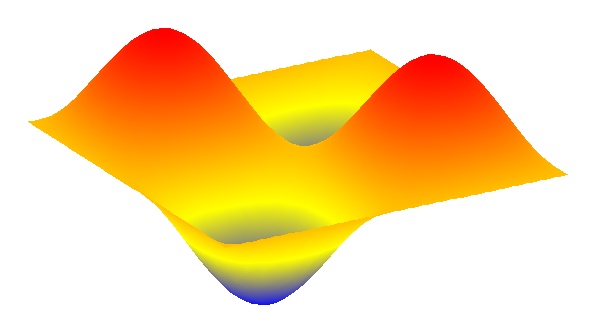
\begin{tikzpicture}
          \begin{axis}[
            view={60}{30},
            hide axis,
            domain=-3.1415:3.1415,
            samples=50,
            samples y=50,
            colormap/hot,
            shader=interp,
          ]
            \addplot3[surf]
              {sin(deg(x)) * sin(deg(y))};
          \end{axis}
        \end{tikzpicture}
    }    
        % Vertical spacing after
        \vspace*{\fill}
    \end{center}
\end{titlepage}

\tableofcontents



\chapter{Partial Differential Equations in Engineering}

\section{Fundamental Lemma of ODEs}

If 
\[
\iiint\limits_{V} f \,d\tau = 0
\quad\text{and}\quad
\begin{aligned}
1.\;& f\text{ is continuous},\\
2.\;& V\text{ is arbitrary},
\end{aligned}
\]
then \(f = 0\) (taken as a fact).

\emph{Proof by contradiction:}

Assume \(f \neq 0\) at a point \(P\).  Because \(f\) is continuous, there is a small volume \(\Delta V\) surrounding \(P\) in which \(f\neq 0\).  (Without loss of generality, assume \(f>0\) rather than \(f<0\).)  

Then 
\[
\iiint_{\Delta V} f \,d\tau > 0,
\]
contradicting the hypothesis that 
\(\iiint_{V} f\,d\tau = 0\).

\begin{center}
\tikzset{every picture/.style={line width=0.75pt}}
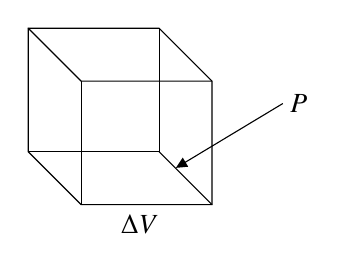
\begin{tikzpicture}[x=0.75pt,y=0.75pt,yscale=-1,xscale=1]
\draw   (248.55,123.49) -- (223.05,97.99) -- (160,97.99) -- (160,157.49) -- (185.5,182.99) -- (248.55,182.99) -- cycle ; \draw   (160,97.99) -- (185.5,123.49) -- (248.55,123.49) ; \draw   (185.5,123.49) -- (185.5,182.99) ;
\draw    (223.05,157.49) -- (160,157.49) ;
\draw    (223.05,157.49) -- (223.05,97.99) ;
\draw    (248.55,182.99) -- (223.05,157.49) ;
\draw    (282.66,134.27) -- (233.73,163.73) ;
\draw [shift={(231.16,165.27)}, rotate = 328.95] [fill={rgb, 255:red, 0; green, 0; blue, 0 }  ][line width=0.08]  [draw opacity=0] (5.36,-2.57) -- (0,0) -- (5.36,2.57) -- cycle    ;
\draw (213.5,186.39) node [anchor=north] [inner sep=0.75pt]    {$\Delta V$};
\draw (284.66,134.27) node [anchor=west] [inner sep=0.75pt]    {$P$};
\end{tikzpicture}
\end{center}

\section{Fluid Flow}

Let $S$ be a closed surface bounding a volume~$V$:

\begin{center}
\tikzset{every picture/.style={line width=0.75pt}} 
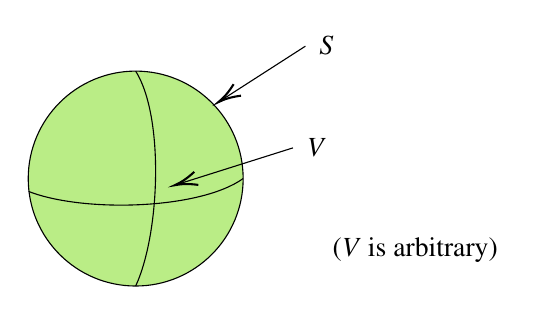
\begin{tikzpicture}[x=0.75pt,y=0.75pt,yscale=-1,xscale=1]
  % (TikZ code unchanged)
  \draw  [fill={rgb,255:red,186;green,237;blue,134},fill opacity=1] 
    (98,123.77) .. controls (98,95.18) and (121.18,72) .. (149.77,72) 
    .. controls (178.37,72) and (201.55,95.18) .. (201.55,123.77) 
    .. controls (201.55,152.37) and (178.37,175.55) .. (149.77,175.55) 
    .. controls (121.18,175.55) and (98,152.37) .. (98,123.77) -- cycle;
  \draw    (149.77,72) .. controls (163.55,93.99) and (161.55,149.99) .. (149.77,175.55);
  \draw    (201.55,123.77) .. controls (180.42,138.84) and (124.4,140.2) .. (98.19,129.99);
  \draw    (231.55,59.99) -- (191.23,85.91);
  \draw [shift={(189.55,86.99)},rotate=327.26] 
         [color={rgb,255:red,0;green,0;blue,0}][line width=0.75]
         (10.93,-3.29) .. controls (6.95,-1.4) and (3.31,-0.3) .. (0,0) 
         .. controls (3.31,0.3) and (6.95,1.4) .. (10.93,3.29);
  \draw    (225.55,108.99) -- (170.45,126.39);
  \draw [shift={(168.55,126.99)},rotate=342.47]
         [color={rgb,255:red,0;green,0;blue,0}][line width=0.75]
         (10.93,-3.29) .. controls (6.95,-1.4) and (3.31,-0.3) .. (0,0) 
         .. controls (3.31,0.3) and (6.95,1.4) .. (10.93,3.29);
  \node at (233.55,59.99)  [anchor=west]          {$S$};
  \node at (227.55,108.99) [anchor=west]          {$V$};
  \node at (240,147.4)     [anchor=north west]    {$(V\text{ is arbitrary})$};
\end{tikzpicture}
\end{center}

\bigskip

\noindent\textbf{Conservation of Mass:}
\[
(3) \;=\; (1)\;+\;(2),
\]
where
\[
M = \iiint_V \delta \,d\tau,
\quad
\frac{dM}{dt} = \iiint_V \frac{\partial\delta}{\partial t}\,d\tau.
\]

\begin{enumerate}
  \item[(1)] \emph{Net mass flux across~$S$:}
  \[
    (1)
    = -\oiint_S \delta\,\mathbf v\!\cdot\!\mathbf n \,dS.
  \]
  \begin{center}
    \tikzset{every picture/.style={line width=0.75pt}} 
    \begin{tikzpicture}[x=0.55pt,y=0.55pt,yscale=-1,xscale=1]
      % (TikZ code unchanged)
      \draw   (158.55,138.99) -- (291.96,138.99) -- (214.73,197.99) -- (81.31,197.99) -- cycle ;
      \draw    (167.55,165.99) -- (146.04,81.93) ;
      \draw [shift={(145.55,79.99)},rotate=75.65]
             [color={rgb,255:red,0;green,0;blue,0}][line width=0.75]
             (10.93,-3.29) .. controls (6.95,-1.4) and (3.31,-0.3) .. (0,0)
             .. controls (3.31,0.3) and (6.95,1.4) .. (10.93,3.29);
      \node at (169.55,165.99) [anchor=west]        {$P$};
      \node at (147.55,76.59)  [anchor=south west]   {$\mathbf v$};
      \node at (81.31,201.39)  [anchor=north]        {$\Delta S$};
    \end{tikzpicture}
  \end{center}

  \item[(2)] \emph{Net generation/absorption in~$V$:}
  \[
    (2)
    = \iiint_V Q(\mathbf r, t)\,d\tau,
  \]
  where $Q$ has units of mass/(volume·time).
\end{enumerate}

\noindent By the Divergence Theorem,
\[
(1)
= -\oiint_S \delta\,\mathbf v\!\cdot\!\mathbf n \,dS
= -\iiint_V \nabla\!\cdot(\delta\,\mathbf v)\,d\tau.
\]
Combining with (2) and the time derivative,
\[
\iiint_V
\Bigl[
\underbrace{\frac{\partial\delta}{\partial t}}_{(3)}
+ \underbrace{\nabla\!\cdot(\delta\,\mathbf v)}_{(1')}
- \underbrace{Q}_{(2)}
\Bigr]
\,d\tau
=0.
\]
By the Fundamental Lemma,
\[
\frac{\partial\delta}{\partial t}
+ \nabla\!\cdot(\delta\,\mathbf v)
- Q = 0
\quad\text{(Law of Conservation of Mass).}
\]

\medskip
\noindent\textbf{Special cases:}
\begin{itemize}
  \item \emph{Incompressible flow} ($\delta=\mathrm{const}$):
    \[
      \nabla\!\cdot\mathbf v \;=\; \frac{Q}{\delta}.
    \]
  \item \emph{Irrotational flow} ($\nabla\times\mathbf v=\mathbf0$):
    set $\mathbf v=\nabla\psi$, yielding
    \[
      \nabla^2\psi = \frac{Q}{\delta}
      \quad\text{(Poisson's equation).}
    \]
    If $Q=0$, this reduces to
    \[
      \nabla^2\psi = 0
      \quad\text{(Laplace's equation).}
    \]
\end{itemize}


\section{Diffusion of Heat}

Let $\psi(\mathbf r, t)$ be the temperature at point $\mathbf r$ and time~$t$.  Let $S$ be a closed surface bounding the volume~$V$:

\begin{center}
\tikzset{every picture/.style={line width=0.75pt}} 
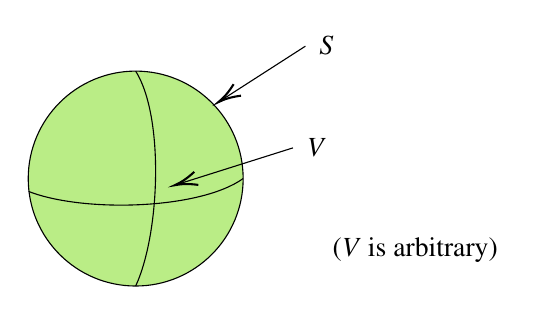
\begin{tikzpicture}[x=0.75pt,y=0.75pt,yscale=-1,xscale=1]
  % (TikZ code unchanged)
  \draw  [fill={rgb,255:red,186;green,237;blue,134},fill opacity=1] 
    (98,123.77) .. controls (98,95.18) and (121.18,72) .. (149.77,72) 
    .. controls (178.37,72) and (201.55,95.18) .. (201.55,123.77) 
    .. controls (201.55,152.37) and (178.37,175.55) .. (149.77,175.55) 
    .. controls (121.18,175.55) and (98,152.37) .. (98,123.77) -- cycle;
  \draw    (149.77,72) .. controls (163.55,93.99) and (161.55,149.99) .. (149.77,175.55);
  \draw    (201.55,123.77) .. controls (180.42,138.84) and (124.4,140.2) .. (98.19,129.99);
  \draw    (231.55,59.99) -- (191.23,85.91);
  \draw [shift={(189.55,86.99)},rotate=327.26] 
         [color={rgb,255:red,0;green,0;blue,0}][line width=0.75]
         (10.93,-3.29) .. controls (6.95,-1.4) and (3.31,-0.3) .. (0,0)
         .. controls (3.31,0.3) and (6.95,1.4) .. (10.93,3.29);
  \draw    (225.55,108.99) -- (170.45,126.39);
  \draw [shift={(168.55,126.99)},rotate=342.47]
         [color={rgb,255:red,0;green,0;blue,0}][line width=0.75]
         (10.93,-3.29) .. controls (6.95,-1.4) and (3.31,-0.3) .. (0,0)
         .. controls (3.31,0.3) and (6.95,1.4) .. (10.93,3.29);
  \node at (233.55,59.99)  [anchor=west]       {$S$};
  \node at (227.55,108.99) [anchor=west]       {$V$};
  \node at (240,147.4)     [anchor=north west] {$(V\text{ is arbitrary})$};
\end{tikzpicture}
\end{center}

\bigskip

\noindent\textbf{Conservation of Energy:}
\[
(3) \;=\; (1)\;+\;(2).
\]
To see this, note:

\medskip
\noindent\emph{Heat in a small mass element.}  A mass $\Delta m$ occupies volume $\Delta\tau$, so $\Delta m=\delta\,\Delta\tau$.  Its thermal energy is
\[
[c\,\psi(\mathbf r,t)\,\delta]_{P}\,\Delta\tau.
\]
Hence the total heat in $V$ is
\[
H \;=\;\iiint_V c\,\delta\,\psi\,d\tau,
\quad
\frac{dH}{dt}
= \iiint_V c\,\delta\,\frac{\partial\psi}{\partial t}\,d\tau.
\]

\begin{enumerate}
  \item[(1)] \emph{Net heat flux across~$S$:}
  \[
    (1)
    = -\oiint_S K\,\nabla\psi\!\cdot\!\mathbf n\,dS.
  \]
  \begin{center}
    \tikzset{every picture/.style={line width=0.75pt}} 
    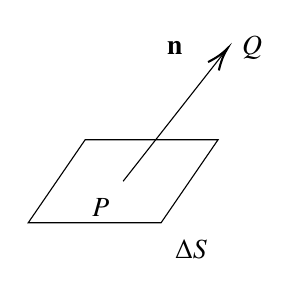
\begin{tikzpicture}[x=0.75pt,y=0.75pt,yscale=-1,xscale=1]
      % (TikZ code unchanged)
      \draw   (105.98,127) -- (170,127) -- (142.56,167) -- (78.55,167) -- cycle;
      \draw    (124.27,147) -- (173.31,84.56);
      \draw [shift={(174.55,82.99)},rotate=128.15]
             [color={rgb,255:red,0;green,0;blue,0}][line width=0.75]
             (10.93,-3.29) .. controls (6.95,-1.4) and (3.31,-0.3) .. (0,0)
             .. controls (3.31,0.3) and (6.95,1.4) .. (10.93,3.29);
      \node at (157.55,82.99) [anchor=east]        {$\mathbf n$};
      \node at (176.55,82.99) [anchor=west]        {$Q$};
      \node at (122.27,150.4) [anchor=north east]  {$P$};
      \node at (144.56,170.4) [anchor=north west]  {$\Delta S$};
    \end{tikzpicture}
  \end{center}

  \item[(2)] \emph{Internal heat generation/absorption:}
  \[
    (2)
    = \iiint_V Q(\mathbf r, t)\,d\tau.
  \]
\end{enumerate}

\noindent By the Divergence Theorem,
\[
(1)
= -\oiint_S K\,\nabla\psi\!\cdot\!\mathbf n\,dS
= -\iiint_V \nabla\!\cdot\bigl(K\,\nabla\psi\bigr)\,d\tau.
\]
Putting it all together,
\[
\iiint_V
\Bigl[
c\,\delta\,\tfrac{\partial\psi}{\partial t}
- \nabla\!\cdot\bigl(K\,\nabla\psi\bigr)
- Q(\mathbf r, t)
\Bigr]
\,d\tau
=0,
\]
so
\[
c\,\delta\,\tfrac{\partial\psi}{\partial t}
- \nabla\!\cdot\bigl(K\,\nabla\psi\bigr)
- Q(\mathbf r, t)
=0.
\]

\medskip
\noindent\textbf{Constant coefficients:} if $c,K,\delta$ are constant,
\[
\frac{1}{\alpha^2}\,\psi_t
- \nabla^2\psi
= \frac{Q}{K},
\quad
\alpha^2 = \frac{K}{\delta\,c}
\quad\text{(``Fourier diffusion equation'').}
\]
In special cases:
\begin{itemize}
  \item $Q=0$: $\displaystyle \frac{1}{\alpha^2}\,\psi_t - \nabla^2\psi = 0.$
  \item Steady state ($\psi_t=0$):
    \[
      \nabla^2\psi = -\,\frac{Q}{K}
      \quad\text{(Poisson's equation).}
    \]
  \item Further, if $Q=0$ in steady state:
    \[
      \nabla^2\psi = 0
      \quad\text{(Laplace's equation).}
    \]
\end{itemize}

\section{Vibrating String}

\begin{center}
\tikzset{every picture/.style={line width=0.75pt}} 
\begin{tikzpicture}[x=0.75pt,y=0.75pt,yscale=-1,xscale=1]
\draw    (104.55,139.99) -- (376.55,139.99) ;
\draw    (105.55,164.99) -- (105.55,95.99) ;
\draw    (104.55,139.99) .. controls (122.55,116.99) and (129.55,102.99) .. (145.55,106.99) .. controls (161.55,110.99) and (171.27,163.35) .. (199.55,167.99) .. controls (227.82,172.63) and (240.34,113.36) .. (259.55,107.99) .. controls (278.75,102.62) and (284.45,156.69) .. (304.55,159.99) .. controls (324.64,163.29) and (341.22,123.73) .. (347.55,118.99) ;
\draw (103.55,92.59) node [anchor=south east] [inner sep=0.75pt]    {$\psi $};
\draw (376.55,143.39) node [anchor=north] [inner sep=0.75pt]    {$x=l$};
\draw (105.55,168.39) node [anchor=north] [inner sep=0.75pt]    {$x=0$};
\end{tikzpicture}
\end{center}

Displacement $\psi$ is a function of time and position

$a^2\dfrac{\partial^2\psi}{\partial x^2}-\dfrac{\partial^2}{\partial t^2}=-F$

$F=\dfrac{\text{Force}}{\text{Mass}},\quad a=\sqrt{\dfrac{T}{\delta}}$

$T$ = Tension\\
$\delta$ = Linear Density\\

General solution to the PDE is: $\psi=\underbrace{F(x-a t)}_{\text{moving right}}+\underbrace{G(x+a t)}_{\text{moving left}}$ ``with speed $a$''

For an ``infinite'' string:

$\psi(x, t)=\dfrac{f(x-a t)+f(x+a t)}{2}+\dfrac{1}{2 a} \displaystyle\int_{x-a t}^{x+a t} g(\xi) d \xi,$ I.C. $\begin{array}{l}
     \psi(x,0)=f(x)  \\
     \psi(t,0)=g(x)
\end{array}$

e.g $f(x)=\sin(x)\quad g(x)=xe^{-x^2}$

$\begin{aligned}
    & \psi(x, t)=\dfrac{\sin (x-a t)+\sin (x+a t)}{2}+\dfrac{1}{2 a} \displaystyle\int_{x-a t}^{x+a t} \xi x e^{-\xi^{2}} d \xi\\
    & =\sin (x) \cos (a t)-\dfrac{1}{4 a}\left[e^{-\xi^{2}}\right]_{x-a t}^{x+a t}
\end{aligned}$


\section{Vibrating Membrane}


$F=m a$ and external forces $\Rightarrow \oiint$

Tension forces $\Rightarrow \oint$

For static deflections: $\dfrac{\partial^{2} \psi}{\partial t^{2}}=0$

strings (1D): $a \dfrac{\partial^{2} \psi}{\partial x^{2}}=-F$

membranes (2D): $\left.\nabla^{2} \psi=-F / a^{2}\right\}$ ``Poisson's Equation''

\section{Three Fundamental Equations}
There are three significant PDEs that govern many engineering systems
\begin{enumerate}
  \item Poisson's Equation

  $\left.\nabla^{2} \psi=-F\right\}$ if 0, Laplace's (special case of Poisson's).
  
  \item Diffusion Equation

  $\nabla^{2} \psi-\dfrac{1}{\alpha^{2}} \dfrac{\partial \psi}{\partial t}=-F$

  \item Wave Equation

  $a^{2} \nabla^{2} \psi-\dfrac{\partial^{2} \psi}{\partial t^{2}}=-F$
\end{enumerate}


Many (but not all) PDEs are governed by one of these 3 equations.

\section{Solving PDEs}

For the homogeneous Wave equation: 

$a^{2} \dfrac{\partial^{2} \psi}{\partial x^{2}}-\dfrac{\partial^{2} \psi}{\partial t^{2}}=0, \quad$ we have a general solution.

$$\psi(x,t)=F(x-at)+G(x+at)$$

Eg. $\begin{array}[t]{lll}
     f(z) & = & z^{2}=(x+i y)^{2}\\
     & = & x^{2}+2 i x y-y^{2}\\
     & = & x^{2}-y^{2}+i(2 x y)=u(x, y)+i v(x, y)
\end{array}$

$\left.\begin{array}{l}
     u(x, y)=x^{2}-y^{2}\\
     v(x, y)=2 x y     
\end{array}\right\}\quad \begin{array}{l}
     \nabla^{2} u=2-2=0\\
     \nabla^{2} v=0 
\end{array}$

The two functions generates two harmonics. This is common. For a well-posed problem, we need a unique solution

\textbf{1. Dirichlet B.C.}

Value of $u$ is constant with time on boundary.

\begin{center}
\tikzset{every picture/.style={line width=0.75pt}}
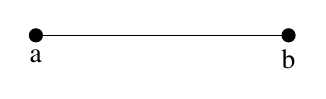
\begin{tikzpicture}[x=0.55pt,y=0.55pt,yscale=-1,xscale=1]
\draw  [draw opacity=0][fill={rgb, 255:red, 0; green, 0; blue, 0 }  ,fill opacity=1 ] (95.34,103) .. controls (95.34,100.43) and (97.43,98.34) .. (100,98.34) .. controls (102.57,98.34) and (104.66,100.43) .. (104.66,103) .. controls (104.66,105.57) and (102.57,107.66) .. (100,107.66) .. controls (97.43,107.66) and (95.34,105.57) .. (95.34,103) -- cycle ;
\draw  [draw opacity=0][fill={rgb, 255:red, 0; green, 0; blue, 0 }  ,fill opacity=1 ] (261.34,103) .. controls (261.34,100.43) and (263.43,98.34) .. (266,98.34) .. controls (268.58,98.34) and (270.66,100.43) .. (270.66,103) .. controls (270.66,105.57) and (268.58,107.66) .. (266,107.66) .. controls (263.43,107.66) and (261.34,105.57) .. (261.34,103) -- cycle ;
\draw    (100,103) -- (266,103) ;
\draw (100,110.66) node [anchor=north] [inner sep=0.75pt]   [align=left] {a};
\draw (266,110.66) node [anchor=north] [inner sep=0.75pt]   [align=left] {b};
\end{tikzpicture}
\end{center}

$$
\left\{\begin{array}{l}
u(a, t)=0 \\
u(b, t)=0
\end{array}\right. \quad \forall t.
$$

\textbf{2. Neumann B.C.}

Spatial derivative of $u$ is constant with time on boundary.

\begin{center}
\tikzset{every picture/.style={line width=0.75pt}} 
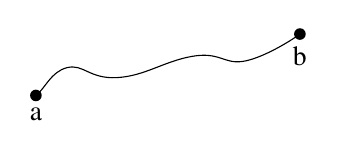
\begin{tikzpicture}[x=0.45pt,y=0.45pt,yscale=-1,xscale=1]
\draw    (133,166) .. controls (140.65,160.26) and (144.91,147.01) .. (158,143.68) .. controls (171.09,140.35) and (175.85,152.84) .. (198,151.68) .. controls (220.16,150.51) and (235.57,138.74) .. (258,134.68) .. controls (280.44,130.61) and (283.83,140.87) .. (299,138.68) .. controls (314.18,136.48) and (337.2,122.53) .. (345,116.68) ;
\draw  [draw opacity=0][fill={rgb, 255:red, 0; green, 0; blue, 0 }  ,fill opacity=1 ] (128.34,166) .. controls (128.34,163.43) and (130.43,161.34) .. (133,161.34) .. controls (135.57,161.34) and (137.66,163.43) .. (137.66,166) .. controls (137.66,168.57) and (135.57,170.66) .. (133,170.66) .. controls (130.43,170.66) and (128.34,168.57) .. (128.34,166) -- cycle ;
\draw  [draw opacity=0][fill={rgb, 255:red, 0; green, 0; blue, 0 }  ,fill opacity=1 ] (340.34,116.68) .. controls (340.34,114.1) and (342.43,112.02) .. (345,112.02) .. controls (347.58,112.02) and (349.66,114.1) .. (349.66,116.68) .. controls (349.66,119.25) and (347.58,121.34) .. (345,121.34) .. controls (342.43,121.34) and (340.34,119.25) .. (340.34,116.68) -- cycle ;
\draw (133,173.66) node [anchor=north] [inner sep=0.75pt]   [align=left] {a};
\draw (345,124.34) node [anchor=north] [inner sep=0.75pt]   [align=left] {b};
\end{tikzpicture}
\end{center}

$$
\left\{\begin{array}{l}
u_{x}(a, t)=0 \\
u_{x}(b, t)=0
\end{array} \quad \forall t\right.
$$

\textbf{3. Robin B.C.}

A linear combination of Dirichelet and Neumann.

$$
A u(a, t)+B u_{x}(a, t)=c, \quad \forall t
$$

\section{Uniqueness Theorems}

``For Poisson's Equation (or Laplace's), the solution of a Dirichlet problem is unique, and Neumann problem is unique to an additive constant."


\textbf{Proof:} Let $\psi_{1}$ and $\psi_{2}$ be two solutions to the same problem, i.e:

$\nabla^{2} \psi_{1}=-F$ and $\left.\nabla^{2} \psi_{2}=-F\right\}$\qquad Goal: Prove $\psi_{1}=\psi_{2}$ for Dirichlet and $\psi_{1}-\psi_{2}=c$ for Neumann

either $\left[\Psi_{1}\right]_{s}=\left[\psi_{2}\right]_{s}$ (Dirichlet) 

or $\left[\dfrac{\partial \psi_{1}}{\partial n}\right]_{s}=\left[\dfrac{\partial \psi_{2}}{\partial n}\right]_{s}$ (Neumann)

Let $u=\psi_{1}-\psi_{2}$, then $\nabla^{2} u=\nabla^{2} \psi_{1}-\nabla^{2} \psi_{2}=-F-(-F)=0$ on $\tau.$

Either $[u]_{s}=0$ (Dirichlet) 
or. 

$\left[\dfrac{\partial u}{\partial n}\right]_{S}=0$ (Neumann)

for this to hold true.

Consider $\oiint\limits_{s} u \dfrac{\partial u}{\partial n} d S=0$, this is equal to $\oiint\limits_{s} u \overrightarrow{\nabla u} \cdot \vec{n} d S \quad$ (Def. of Del operator).

Applying Divergence Theorem:

$0=\iiint\limits_{\tau} \vec{\nabla} \cdot[u \overrightarrow{\nabla u}] d \tau \quad$ Apply vector identity (Product Rule) from Tutorial 1 .


$0=\iiint\limits_{\tau} \underbrace{\overrightarrow{\nabla u} \cdot \overrightarrow{\nabla u}}_{\|\overrightarrow{\nabla u}\|^{2}} d \tau+\iiint\limits_{\tau} u \underbrace{\nabla^{2} u}_{=0} d \tau
$

However, we may not automatically conclude $\|\overrightarrow{\nabla u}\|^{2}=0$ by the Fundamental Lemma since $\tau$ is not arbitrary. Why is it not arbitrary? We have restricted our analysis to Dirichlet or Neumann B.C.s, rather than \textit{any} boundary conditions. 

Instead, we use the limit of a sum argument for integrals because $\|\overrightarrow{\nabla u}\|^{2} \geqslant 0$.

And $\iiint\limits_{\tau} \underbrace{\|\vec{\nabla u}\|^{2}}_{\geq 0} d \tau=0 \quad$ 

$\therefore\|\overrightarrow{\nabla u}\|^2=0$ in $\tau$

$\therefore\overrightarrow{\nabla u}=0\quad\Rightarrow\quad u=\psi_1-\psi_2=c$ in $\tau$.

This proves the Neumann part.

For Dirichlet, we have $[u]_{s}=0$ and $[u]_{\tau}=c$

Since $\tau$ can be infinitesimally close to $s$, we can't continuously go from 0 on $S$ to $c$ on $\tau$, if $c \neq 0$ $\therefore c=0 \Rightarrow \psi_{1}=\psi_{2}$, which proves the Dirichlet case.

Note on arbitrary domains:

Consider $\displaystyle\int_{\tau} x d x$. This is clearly not always zero. However, if domain $\tau=x \in[-1,1]$, then $\displaystyle\int_{-1}^{1} x d x=0$. This doesn't mean $x$ is zero, since the domain is not arbitrary. This is the definition of ``arbitrary $\tau$'' in the Fundamental Lemma. It can only be applied if the domain is arbitrary (and thus integral = 0 regardless of bounds).

``For Poisson's Equation (or Laplace's), the solution of a Robin problem is unique.

\textbf{Proof:} Let $\psi_{1}$ and $\psi_{2}$ be two solutions to the same problem, i.e:

$\nabla^{2} \psi_{1}=-F$ and $\nabla^{2} \psi_{2}=-F$ in $\tau$.

$\dfrac{\partial \psi_{1}}{\partial n}+h \psi_{1}=\dfrac{\partial \psi_{2}}{\partial n}+h \psi_{2}$ on $s$. the boundary of $\tau$, with $h$ positive.

Let $u=\psi_{1}-\psi_{2}$, then $\nabla^{2} u=0$ in $\tau$.

$$
\dfrac{\partial}{\partial n}\left(\psi_{1}-\psi_{2}\right)+h\left(\psi_{1}-\psi_{2}\right)=0 \text { or } \frac{\partial u}{\partial n}+h u=0 \text { on } S .
$$

Now, $\oiint\limits_{s} u \dfrac{\partial u}{\partial n} d S=-\oiint\limits_{s} h u^{2} d S \quad\left(\frac{\partial u}{\partial n}=-h u\right)$

$$
=\oiint_{s} u \overrightarrow{\nabla u} \cdot \stackrel{\rightharpoonup}{n} d S \Rightarrow\iiint_{\tau} \vec{\nabla} \cdot(u \overrightarrow{\nabla u}) d \tau \text { (by the Divergence Theorem) }
$$

$$
\therefore -\oiint_{S} h\,u^{2} \, dS 
= \iiint_{\tau} \nabla \cdot \bigl(u\,\nabla u\bigr)\, d\tau
= \iiint_\tau 
  \underbrace{\nabla u \cdot \nabla u}_{\|\nabla u\|^2 \geqslant 0} 
  \, d\tau.
+ \cancel{\iiint_{\tau} u\,\nabla^{2}u \, d\tau}
\text{ (Poisson problem: } \nabla^{2}u = 0\text{) }
$$

Only way for L.H.S. = R.H.S. is if both are $0$.

The gist of this proof is that the L.H.S. $\leqslant 0$ and the R.H.S. is $\geqslant 0$. The only way for this to be possible is if L.H.S = R.H.S. = 0.

$\iiint\limits_{\tau}\|\overrightarrow{\nabla u}\|^{2} d \tau=0 \Rightarrow u=$ constant in $\tau$.

$$
\oiint_{S} \underbrace{h u^{2}}_{\geqslant 0} d s=0 \Rightarrow u=0 \text { on } S.
$$

Hence by continuity, $u=\psi_{1}-\psi_{2}=0$, thus $\psi_{1}=\psi_{2}$.

Theorem 3: For the diffusion equation, solutions of Dirichlet and Neumann problems are unique if $\psi(\vec{r}, 0)$ is specified.

Theorem 4: For the wave equation, solutions of Dirichlet and Neumann problems are unique if $\psi(\vec{r}, 0)$ and $\psi_{+}(\vec{r}, 0)$ is specified.

(Proofs not needed).

%%%%%%%%%%%%%%%%%%%%%%

%%%%%%%%%%%%%%%%%%%%%%%


\chapter{Boundary Value Problems}

\section{BVP 1(A): Diffusion of Heat in a Thin Bar, Ends Maintained at $0^\circ$}

Thin rod of length $L$, ends maintained at $0^\circ$, initial temperature $f(x)$, no heat generation, or absorption.\\

\begin{center}
    \begin{tabular}{cc}
    \tikzset{every picture/.style={line width=0.75pt}} 
    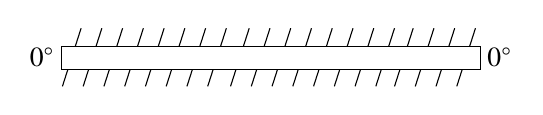
\begin{tikzpicture}[x=0.75pt,y=0.75pt,yscale=-1,xscale=1]
    \draw    (126.5,104) -- (117.5,132) ;
    \draw    (136.5,104) -- (127.5,132) ;
    \draw    (146.5,104) -- (137.5,132) ;
    \draw    (156.5,104) -- (147.5,132) ;
    \draw    (166.5,104) -- (157.5,132) ;
    \draw    (176.5,104) -- (167.5,132) ;
    \draw    (186.5,104) -- (177.5,132) ;
    \draw    (196.5,104) -- (187.5,132) ;
    \draw    (207.5,104) -- (198.5,132) ;
    \draw    (217.5,104) -- (208.5,132) ;
    \draw    (227.5,104) -- (218.5,132) ;
    \draw    (237.5,104) -- (228.5,132) ;
    \draw    (247.5,104) -- (238.5,132) ;
    \draw    (257.5,104) -- (248.5,132) ;
    \draw    (267.5,104) -- (258.5,132) ;
    \draw    (277.5,104) -- (268.5,132) ;
    \draw    (286.5,104) -- (277.5,132) ;
    \draw    (296.5,104) -- (287.5,132) ;
    \draw    (306.5,104) -- (297.5,132) ;
    \draw    (316.5,104) -- (307.5,132) ;
    \draw  [fill={rgb, 255:red, 255; green, 255; blue, 255 }  ,fill opacity=1 ] (117,113) -- (319,113) -- (319,124) -- (117,124) -- cycle ;
    \draw (115,118) node [anchor=east] [inner sep=0.75pt]    {$0^{\circ }$};
    \draw (321,118) node [anchor=west] [inner sep=0.75pt]    {$0^{\circ }$};
    \end{tikzpicture} & \raisebox{0.25cm}
    {}
    \end{tabular}
\end{center}

$$
\psi(0,t) = 0, \quad \psi(L,t) = 0, \quad \psi(x,0) = f(x)
$$

Start with the Diffusion Equation:

$$
\dfrac{1}{\alpha^2} \dfrac{\partial \psi}{\partial t} - \nabla^2 \psi = \dfrac{Q}{K}\qquad Q=0\text{ \textit{bc. no heat generation or absorption}}
$$

* \textit{"Thin" implies temperature is independent of $y$ and $z$ $\left(\frac{\partial \psi}{\partial y} = 0\right)$.}

As there is no heat generation, the diffusion equation becomes:

$$
\dfrac{1}{\alpha^2} \dfrac{\partial \psi}{\partial t} = \dfrac{\partial^2 \psi}{\partial x^2}, \quad 0 < x < L, \, t > 0\quad\longrightarrow\quad \text{\textit{Heat equation with Dirichlet B.C.s (MATH 264)}}
$$

We have\\

\begin{tabular}{lll}
     & B.C.s: & $\psi(0,t) = 0, \quad \psi(L,t) = 0$  \\
     & \\
\end{tabular}

And\\

\begin{tabular}{lll}
     & I.C.: & $\psi(x,0) = f(x)$\\
     & \\
\end{tabular}

Recall solving separable PDEs in MATH 264, look for solutions of the form:\\

\begin{tabular}{ll}
     & $u(x,t) = T(t)X(x),\quad \text{\textit{Plug into PDE:}}$ \\
     & \\
     & $\dfrac{1}{\alpha^2} \dfrac{dT}{dt} = T \cdot \dfrac{d^2X}{dx^2},\quad \text{\textit{Move all $X$ terms to one side, all $T$ terms to other side.}}$\\
     &\\
     & $\left.\dfrac{1}{\alpha^2 T}\cdot  \dfrac{dT}{dt} = \dfrac{1}{X}\cdot \dfrac{d^2X}{dx^2} = h(x,t)\right\}$\quad \text{\textit{$h$ = constant $(\lambda)$ because it is independent of $x$ and $t$.}}\\
     &\\
\end{tabular}

Thus, we must solve the 2 ODEs:

\[
\begin{aligned}
\frac{1}{\alpha^2\,T}\,\frac{dT}{dt} &= \lambda,
& \quad & 
\text{Trivially,}\ 
\frac{\partial}{\partial x}\!\Bigl[\tfrac{1}{\alpha^2\,T}\,\tfrac{dT}{dt}\Bigr] = 0,\\[6pt]
\frac{1}{X}\,\frac{d^2X}{dx} &= \lambda,
& \quad &
\text{Trivially,}\ 
\frac{\partial}{\partial t}\!\Bigl[\tfrac{1}{X}\,\tfrac{d^2X}{dx}\Bigr] = 0.
\end{aligned}
\]

$\dfrac{d^2X}{dx^2} + X\lambda,\ X(0)=0,\ X(L)=0$.\quad \textit{$\lambda$ can be 0, +ve, or -ve. (MATH 264)}\\


\textbf{Case 1: $\lambda=0$:}

$$
\frac{d^2X}{dx^2} = 0\quad\Rightarrow\quad \implies X(x) = \parrow{A + Bx}{X(0)=0\quad X(L)=0}\quad\left. \therefore B=0\quad \therefore AL=0\quad\Rightarrow\quad A=0\quad\right\}\text{\textit{Trivial solution}}
$$

\textbf{Case 2: $\lambda +\text{ve},\ \text{ie } \lambda=\mu^2$}

$$
\frac{d^2X}{dx^2} + \mu^2 X = 0
$$

We can express this as \underline{either} $X(x) = C_1 e^{\mu x} + C_2 e^{-\mu x} \quad \text{or} \quad X(x) = K_1 \cosh(\mu x) + K_2 \sinh(\mu x)$

* \textit{These are mathematically equivivalent and interchangeable. Here, we choose the hyperbolics since B.C. $X(0)=0$ kills the cosh term (cleaner)}.

$X(x)=K_1\cosh(\mu x)+K_2\sinh(\mu x)$. $X(0)=0\quad \begin{array}{l}
    *\cosh(0)=1 \\
    *\sinh(0)=0 
\end{array} \quad \therefore K_1=0$

$X(L)=0\quad\Rightarrow\quad K_2\sinh(\mu L)=0\quad\Rightarrow\quad K_2=0\ \}$ Trivial solution, $\sinh$ is never nonzero outside $x=0$... but $\sin$ is.\\

\textbf{Case 3: $\lambda$ - ve, i.e., $\lambda = -\mu^2$}

$$
\frac{d^2X}{dx^2} = - \mu^2 X \quad\Rightarrow\quad X(x) = A \cos(\mu x) + B \sin(\mu x)\quad \therefore A=0\quad \therefore 0=B\sin(\mu L)\quad B\neq 0
$$

Want $\sin(\mu L)=0$

$\therefore \mu L=n\pi,\quad n\in \pm1,\pm 2,\ldots$

$$
\mu=\dfrac{n\pi}{L},\quad \lambda=-\mu^2
$$

$\therefore \lambda=-\dfrac{n^2\pi^2}{L^2}\quad\Rightarrow\quad X_n(x)=B_n\sin\left(\dfrac{n\pi x}{L}\right), n\in\mathbb{N}(1,2,3,\ldots)$

Now we consider:
$$
\frac{1}{\alpha^2} \frac{dT}{dt} = \lambda = -\frac{n^2 \pi^2}{L^2} \text{ with } \lambda=\dfrac{-n^2\pi^2}{L^2}
$$

$\therefore \dfrac{dT}{dt}=\left.\underbrace{-\dfrac{\alpha^2n^2\pi^2}{L^2}}_{\text{constant}}\right.\}\text{recall, } y'=y\quad \Rightarrow\quad y=Ce^x$

$\therefore T_n(t)=C_ne^{-\frac{\alpha^2n^2\pi^2}{L^2}+}$


Combine $\psi_n(x, t) = X_n(x) T_n(t)$:

$$
\psi_n = D_n \sin\left(\frac{n \pi x}{L}\right) \underbrace{e^{-\frac{\alpha^2 n^2 \pi^2}{L^2} t}}_{=1\text{ when }t=0}, \ n \in \mathbb{N}.\quad \text{\textit{We must now find $D_n$ using I.C. $\psi(x, 0) = f(x)$}}
$$

$$
D_n\sin\left(\dfrac{n\pi x}{L}\right)=f(x)
$$

Can't resolve this unless $f(x)$ is a multiple of $\sin\left(\frac{n \pi x}{L}\right)$, which is a very rare edge case.

So we write the general:

$$
\underbrace{\left[\frac{1}{\alpha^2} \frac{\partial}{\partial t} - \frac{\partial^2}{\partial x^2}\right]}_{\mathcal{L}} (\psi(x, t)) = 0\quad \therefore \mathcal{L}\psi = 0.
$$

We want the nullspace of this (linear) operator $\mathcal{L}$.

By superposition, if $\psi_1, \psi_2, \dots$ are solutions, so is their sum:

$$
\therefore \psi(x, t) = \sum\limits_{n=1}^N \psi_n(x, t)
$$

$$
f(x) = \sum\limits_{n=1}^N D_n \sin\left(\dfrac{n \pi x}{L}\right) = \psi(x, 0).
$$

A solution for this exists for all piecewise smooth functions ($f(x)$, $f'(x)$ piecewise continuous, may have jump discontinuities).

For $f(x) = e^{x} =\sum\limits_{n=0}^N \frac{x^n}{n!}$ requires $N \to \infty$, so we must do $N \to \infty$ for all piecewise smooth $f(x)$.

$$
\therefore f(x) = \sum\limits_{n=1}^\infty D_n \sin\left(\dfrac{n \pi x}{L}\right)\quad \text{\textit{We integrate both (Fourier Sine Series):}}
$$


$$
\displaystyle\int_0^L \sin\left(\frac{n \pi x}{L}\right) f(x) \, dx = \sum\limits_{n=1}^\infty D_n \displaystyle\int_0^L \sin\left(\dfrac{n \pi x}{L}\right) \sin\left(\dfrac{n \pi x}{L}\right) \, dx
$$

The RHS integral vanishes whenever $n \neq k$, and is equal to $\frac{L}{2}$ when $n = k$.

Interchanging $n$ and $k$ gives:

\[
\boxed{
D_n = \dfrac{2}{L} \int_0^L \sin\left(\dfrac{n \pi x}{L}\right) f(x) \, dx,\text{ sub into } 
\psi(x,t)=\sum\limits_{n=1}^{\infty} D_n \sin\left(\dfrac{n\pi x}{L}\right) 
e^{-\frac{\alpha^2n^2\pi^2}{L^2}t}
}
\]

Example: $L=\pi,\ f(x)=x(\pi-x)=\psi(x,0)$\\

\begin{center}
\tikzset{every picture/.style={line width=0.75pt}} 
\begin{tikzpicture}[x=0.75pt,y=0.75pt,yscale=-1,xscale=1]
\draw[->]    (97,262) -- (305,262) ;
\draw[->]    (117,282) -- (117,114) ;
\draw    (117,261) .. controls (153,149) and (244,149) .. (276,261) ;
\draw (276,265.4) node [anchor=north] [inner sep=0.75pt]    {$\pi $};
\end{tikzpicture}
\end{center}

$$
\psi(x,t)=\sum\limits_{n=1}^{\infty}D_n\sin(nx)e^{-\alpha^2n^2t}
$$

$$
\psi(x,0)=X(\pi-x)=\dfrac{8}{\pi}\left[\dfrac{\sin(x)}{1^3}+\dfrac{\sin(3x)}{3^3}+\dfrac{\sin(5x)}{5^3}+\ldots\right]
$$

Now, incorporate $T(t)$:

$$
\psi(x,t)=\dfrac{8}{\pi}\left[\dfrac{\sin(x)}{1^3}e^{-\alpha^2t}+\dfrac{\sin(3x)}{3^3}e^{-9\alpha^2t}+\dfrac{\sin(5x)}{5^3}e^{-25\alpha^2t}+\ldots\right]\quad \text{(\textit{Converges rapidly})}
$$

\section{BVP 1(B): Diffusion of Heat in a Thin Bar, Ends Insulated}

$$\dfrac{1}{\alpha^2}\dfrac{\partial \psi}{\partial t}=\dfrac{\partial^2\psi}{\partial x^2},\qquad 0<x<L,\quad t>0$$

$\left.\begin{array}{l}
     \text{B.C.s: } \psi_x(0,t)=0,\quad \psi_x(L,t)=0\\
     \text{I.C.: } \psi(x,0)=f(x) 
\end{array}\right\}$ \textit{Heat equation with Neumann B.Cs (while 1A is Dirichelet)}

Using the same procedure, we get:

$$\psi_n(x,t)=D_n\parrow{\cos}{unlike sin for BVP 1A}\left(\dfrac{n\pi x}{L}\right)e^{-\frac{\alpha^2n^2\pi^2}{L^2}t}\qquad n=\parrow{0}{start at zero because $\cos(0)\neq 0$},1,2,\ldots$$

Once again, the I.C. $\psi(x,0)$ rarely gives a clean solution.

So we once again write the PDE as:

$\left.\left[\dfrac{1}{\alpha^2}\dfrac{\partial}{\partial t}-\dfrac{\partial^2}{\partial x^2}\right]\psi(x,t)=0\right\}\quad\Rightarrow\quad \mathcal{L}\psi=0$\qquad \textit{Want nullspace of $\mathcal{L}$}

$$\psi(x,t)=\sum\limits_{n=0}^{\infty}\psi_n(x,t)=\sum\limits_{n=0}^{\infty}D_n\cos\left(\dfrac{n\pi x}{L}\right)e^{-\frac{\alpha^2n^2\pi^2}{L^2}t}$$

\textit{We extract the $n=0$ term and deal with it separately (In B.V.P 1A irrelevant because $\sin(0)=0$)}

$$\begin{array}{lll}
    \therefore & \psi(x,t)=D_0+\sum\limits_{n=1}^{\infty}D_n\cos\left(\dfrac{n\pi x}{L}e^{-\frac{\alpha^2n^2\pi^2}{L^2}t}\right) & \text{\textit{Apply I.C.}}  \\
     & \psi(x,0)=D_0+\sum\limits_{n=1}^{\infty}D_n\cos\left(\dfrac{n\pi x}{L}\right) =f(x) & \text{\textit{Use Fourier Cosine series}}
\end{array}$$

$\displaystyle\int\limits_0^L\cos\left(\dfrac{k\pi x}{L}\right)f(x)dx=\underbrace{D_0\displaystyle\int_0^L\cos\left(\dfrac{k\pi x}{L}\right)}_{0}dx+\sum\limits_{n=1}^ND_n\underbrace{\displaystyle\int\limits_{0}^L\cos\left(\dfrac{k\pi x}{L}\right)\cos\left(\dfrac{n\pi x}{L}\right)dx}_{\substack{\text{Like BVP 1A. this is = 0}\\
\text{if $n\neq k$ and $=\frac{L}{2}$ if $n=k$}\\
\text{we use the Kronecker Delta}\\
\delta_{kn}=\left\{\begin{array}{ll}
     0 & \text{if } k\neq n  \\
     1 & \text{if } k=n 
\end{array}\right.}}=\dfrac{L}{2}D_k$,

interchange $k$ and $n$.

\begin{equation}\label{eq_1}
    \boxed{
        D_n = \dfrac{2}{L} \int\limits_0^L \cos\left(\dfrac{n\pi x}{L}\right) f(x) \, dx
    }
\end{equation}

%%%%%%%%%%%%%%%%%%%%%%%%%%%%%%%%

In addition, for the $k=0$ case:

\begin{equation}\label{eq_2}
    \displaystyle\int\limits_{0}^{L}(1) f(x) d x=\underbrace{D_{0} \int_{0}^{L}(1) d x}_{L} + \sum\limits_{n=1}^{\infty} D_{n} \underbrace{\displaystyle\int\limits_{0}^{1}(1) \cos \left(\dfrac{n \pi x}{L}\right) d x}_{0}=D_{0} \cdot L
\end{equation}

\[
\therefore \quad \boxed{D_0 = \dfrac{1}{L} \int\limits_0^L f(x) \, dx}
\]

Sub in (\ref{eq_1}) and (\ref{eq_2}) into 
\[
\boxed{
\psi(x, t) = D_{0} + \sum\limits_{n=1}^{\infty} D_{n} \cos \left(\dfrac{n \pi x}{L}\right) 
e^{-\frac{\alpha^{2} n^{2} \pi^{2}}{L^{2}}t}
}
\]
for the solution.

\textbf{Example:} $L=\pi,\ f(x)=x(\pi-x)$

$$
\begin{aligned}
\psi(x, t) & = D_{0}+\sum\limits_{n=1}^{\infty} D_{n} \cos (n x) e^{-\alpha^{2} n^{2} t} \\
\psi(x, 0) & =x(\pi-x)=D_{0}+\sum\limits_{n=1}^{\infty} D_{n} \cos (n x)=\dfrac{\pi^{2}}{6}-\left[\dfrac{\cos (2 x)}{1^{2}}+\dfrac{\cos (4 x)}{2^{2}}+\dfrac{\cos (6 x)}{3^{2}}+\ldots\right. \\
\therefore \psi(x, t) & =\dfrac{\pi^{2}}{6}-\left[\dfrac{\cos (2 x)}{1^{2}} e^{-4 \alpha^{2}+}+\dfrac{\cos (4 x)}{2^{2}} e^{-16 \alpha^{2}+}+\dfrac{\cos (6 x)}{3^{2}} e^{-36 \alpha^{2}+}+\ldots\right. \text { \textit{(converges vapidly,  but slower than 1A).} }
\end{aligned}
$$

The Fourier Sine and Cosine series both extends the domain of $f(x)$, but in different ways.

\begin{center}
\tikzset{every picture/.style={line width=0.75pt}} 
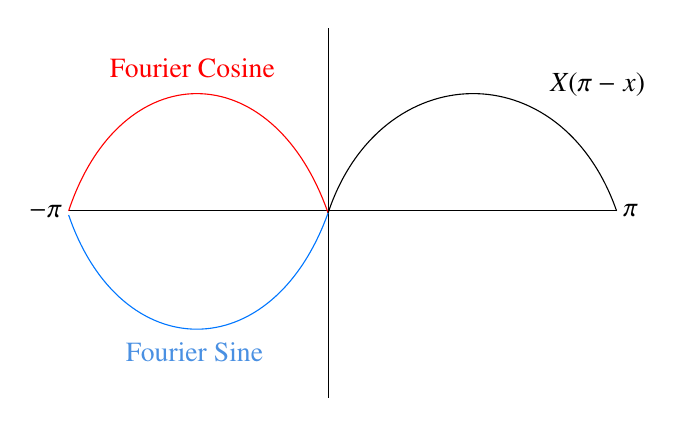
\begin{tikzpicture}[x=0.75pt,y=0.75pt,yscale=-1,xscale=1]
\draw    (104.55,136.99) -- (368.55,136.99) ;
\draw    (229.55,226.99) -- (229.55,48.99) ;
\draw [color={rgb, 255:red, 255; green, 0; blue, 0 }  ,draw opacity=1 ]   (104.55,136.99) .. controls (129.55,61.99) and (202.55,60.99) .. (229.55,137.99) ;
\draw [color={rgb, 255:red, 0; green, 0; blue, 0 }  ,draw opacity=1 ]   (229.55,137.99) .. controls (254.55,62.99) and (341.55,59.99) .. (368.55,136.99) ;
\draw [color={rgb, 255:red, 0; green, 118; blue, 255 }  ,draw opacity=1 ]   (104.55,138.96) .. controls (129.55,212.01) and (202.55,212.98) .. (229.55,137.99) ;
\draw (164.19,73.99) node [anchor=south] [inner sep=0.75pt]  [color={rgb, 255:red, 255; green, 0; blue, 0 }  ,opacity=1 ] [align=left] {Fourier Cosine};
\draw (165.19,199) node [anchor=north] [inner sep=0.75pt]  [color={rgb, 255:red, 74; green, 144; blue, 226 }  ,opacity=1 ] [align=left] {Fourier Sine};
\draw (335,82.98) node [anchor=south west] [inner sep=0.75pt]    {$X( \pi -x)$};
\draw (102.55,136.99) node [anchor=east] [inner sep=0.75pt]    {$-\pi $};
\draw (370.55,136.99) node [anchor=west] [inner sep=0.75pt]    {$\pi $};
\end{tikzpicture}
\end{center}

\section{BVP 2: Vibrating String}

\begin{center}
\tikzset{every picture/.style={line width=0.75pt}}
\begin{tikzpicture}[x=0.75pt,y=0.75pt,yscale=-1,xscale=1]
\draw    (107,180) -- (358,180) ;
\draw [shift={(358,180)}, rotate = 180] [color={rgb, 255:red, 0; green, 0; blue, 0 }  ][line width=0.75]    (0,5.59) -- (0,-5.59)   ;
\draw [shift={(107,180)}, rotate = 180] [color={rgb, 255:red, 0; green, 0; blue, 0 }  ][line width=0.75]    (0,5.59) -- (0,-5.59)   ;
\draw    (107,158) -- (107,70.68) ;
\draw [shift={(107,68.68)}, rotate = 90] [color={rgb, 255:red, 0; green, 0; blue, 0 }  ][line width=0.75]    (10.93,-3.29) .. controls (6.95,-1.4) and (3.31,-0.3) .. (0,0) .. controls (3.31,0.3) and (6.95,1.4) .. (10.93,3.29)   ;
\draw    (107,158) .. controls (113.2,153.35) and (119,141.68) .. (134,141.68) .. controls (149,141.68) and (154.07,163.26) .. (176,166.68) .. controls (197.94,170.09) and (200.47,128.4) .. (217,128.68) .. controls (233.54,128.95) and (218.7,167.85) .. (233,171.68) .. controls (247.31,175.51) and (252.69,133.1) .. (268,131.68) .. controls (283.31,130.26) and (275.18,158.35) .. (286,161.68) .. controls (296.82,165) and (306.53,146.92) .. (323,144.68) .. controls (339.48,142.43) and (354.94,154.98) .. (358,152.68) ;
\draw  [draw opacity=0][fill={rgb, 255:red, 0; green, 0; blue, 0 }  ,fill opacity=1 ] (103.34,161.66) .. controls (103.34,159.64) and (104.98,158) .. (107,158) .. controls (109.02,158) and (110.66,159.64) .. (110.66,161.66) .. controls (110.66,163.68) and (109.02,165.32) .. (107,165.32) .. controls (104.98,165.32) and (103.34,163.68) .. (103.34,161.66) -- cycle ;
\draw  [draw opacity=0][fill={rgb, 255:red, 0; green, 0; blue, 0 }  ,fill opacity=1 ] (350.68,152.68) .. controls (350.68,150.65) and (352.32,149.02) .. (354.34,149.02) .. controls (356.36,149.02) and (358,150.65) .. (358,152.68) .. controls (358,154.7) and (356.36,156.34) .. (354.34,156.34) .. controls (352.32,156.34) and (350.68,154.7) .. (350.68,152.68) -- cycle ;
\draw (105,65.28) node [anchor=south east] [inner sep=0.75pt]    {$\psi $};
\draw (232.5,183.4) node [anchor=north] [inner sep=0.75pt]    {$L$};
\end{tikzpicture}
\end{center}

We now use the Wave Equation 

$\left.a^{2} \dfrac{\partial^{2} \psi}{\partial x^{2}}-\dfrac{\partial^{2} \psi}{\partial t^{2}}=-F\right\} \text { Free vibrations. no external forces. $\therefore\ F=0$}$ 

$\therefore\quad a^{2} \dfrac{\partial^{2} \psi}{\partial x^{2}}=\dfrac{\partial^{2} \psi}{\partial t^{2}}$

We now have the PDE:

$$
\left.\begin{array}{l}
a^{2} \dfrac{\partial^{2} \psi}{\partial x^{2}}=\dfrac{\partial^{2} \psi}{\partial t^{2}} \quad \text { with B.C.s } \\
\psi(0, t)=0,\ \psi(L, t)=0, \text { and I.C.s } \\
\psi(x, 0)=f(x),\ \psi_{t}(x, 0)=g(x)
\end{array}\right\}\text{\textit{Wave Equation with Dirichlet B.C.s}}
$$

Physically, string with fixed/tied ends. Initial displacement of $f(x)$ and initial velocity of $g(x)$. Small vibrations.

Once again, assume $\psi(x, t)=X(x) T(t)$. Plug into PDE:

$$
a^{2} T \dfrac{d^{2} X}{d x^{2}}=X \dfrac{d^{2} T}{d t^{2}}
$$

$\dfrac{1}{X} \dfrac{d^{2} X}{d x^{2}}=\dfrac{1}{a^{2} T} \dfrac{d^{2} T}{d t^{2}}=\lambda$ \textit{This separates to two second-order ODEs}

$$
\dfrac{d^{2} X}{d x^{2}}=\lambda X \quad X(0)=0, X(L)=0
$$

$\left.\begin{array}{l}
     \text{Like in BVP 1A, $\lambda=-\dfrac{n^{2} \pi^{2}}{L^{2}}$ } \\
     X_{n}(x)=A_{n} \sin \left(\dfrac{n \pi x}{L}\right) 
\end{array}\right\}\quad n=1,2, \ldots\text{ because $\sin(0)=0$}.$


$$
\dfrac{d^{2} T}{d t^{2}}=a^{2} \lambda T=-\underbrace{\dfrac{a^{2} n^{2} \pi^{2}}{L^{2}}}_{w_n^2} T,\quad w_{n}=\dfrac{a n \pi}{L}
$$

Allowed angular frequencies of vibration ($n=1,2,3, \ldots$)

$\therefore \dfrac{d^{2} T}{d t^{2}}=-w_{n}^{2} T$ 

General solution is:

$\left.T_{n}(t)=B_{n}^{\prime} \cos \left(w_{n} t\right)+C_{n}^{\prime} \sin \left(w_{n} t\right)\right\}\quad\text { Both $\sin$ and $\cos$ terms exist because $IC \neq B C$, $I C$ is not homogeneous.}$

$$
\psi_{n}(x, t)=\sin \left(\dfrac{n \pi x}{L}\right)\left[B_{n} \cos \left(W_{n} t\right)+C_{n} \sin (W_n t)\right] \begin{aligned}
& B_{n}=B_{n}^{\prime} \cdot A_{n} \\ 
& C_{n}=C'_{n} \cdot A_{n}
\end{aligned}\quad n=1,2, \ldots
$$

Like before, we can rarely satisfy ICs with a single value of $n$. So we use a Fourier Series again

$$
\therefore\underbrace{\left[a^{2} \dfrac{\partial^{2}}{\partial x^{2}}-\dfrac{\partial^{2}}{\partial t^{2}}\right]}_{\mathcal{L}\text{ (a linear operator)}} \psi(x, t)=0\quad \text { find nullspace of } \mathcal{L}.
$$

\[
\boxed{
\psi(x, t) = \sum\limits_{n=1}^{\infty} \sin\left(\dfrac{n \pi x}{L}\right) \left[ B_{n} \cos\left(\omega_{n} t\right) + C_{n} \sin\left(\omega_{n} t\right) \right]
}
\]

Apply position IC for $B_n$:

$\psi(x, 0)=f(x)=\sum\limits_{n=1}^{\infty} B_{n} \sin \left(\dfrac{n \pi x}{L}\right)$ \textit{Using process in BVP 1}:

\[
\boxed{
B_{n} = \dfrac{2}{L} \int\limits_{0}^{L} f{(x)} \sin\left(\dfrac{n \pi x}{L}\right) \, dx
}
\]

Apply velocity IC for $C_{n}$:

\[
\begin{aligned}
\psi_{t}(x, 0) &= \sum\limits_{n=1}^{\infty} C_{n} w_{n} \sin \left( \dfrac{n \pi x}{L} \right) = g(x) \\
\therefore\ & \boxed{ C_{n} w_{n} = \dfrac{2}{L} \int\limits_{0}^{L} g(x) \sin \left( \dfrac{n \pi x}{L} \right) \, dx }
\end{aligned}
\]

Sub in $B_{n}$ and $C_{n}$ for the particular solution.

\section{Newton's Law of Heating and Cooling}

\begin{center}

\tikzset{every picture/.style={line width=0.75pt}}
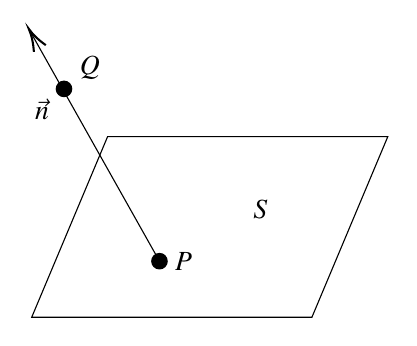
\begin{tikzpicture}[x=0.75pt,y=0.75pt,yscale=-1,xscale=1]
\draw   (136.55,126) -- (271.55,126) -- (235,212.99) -- (100,212.99) -- cycle ;
\draw    (161.55,185.99) -- (99.53,75.73) ;
\draw [shift={(98.55,73.99)}, rotate = 60.64] [color={rgb, 255:red, 0; green, 0; blue, 0 }  ][line width=0.75]    (10.93,-3.29) .. controls (6.95,-1.4) and (3.31,-0.3) .. (0,0) .. controls (3.31,0.3) and (6.95,1.4) .. (10.93,3.29)   ;
\draw  [draw opacity=0][fill={rgb, 255:red, 0; green, 0; blue, 0 }  ,fill opacity=1 ] (157.54,185.99) .. controls (157.54,183.78) and (159.33,181.98) .. (161.55,181.98) .. controls (163.76,181.98) and (165.55,183.78) .. (165.55,185.99) .. controls (165.55,188.2) and (163.76,189.99) .. (161.55,189.99) .. controls (159.33,189.99) and (157.54,188.2) .. (157.54,185.99) -- cycle ;
\draw  [draw opacity=0][fill={rgb, 255:red, 0; green, 0; blue, 0 }  ,fill opacity=1 ] (111.54,102.99) .. controls (111.54,100.78) and (113.33,98.98) .. (115.55,98.98) .. controls (117.76,98.98) and (119.55,100.78) .. (119.55,102.99) .. controls (119.55,105.2) and (117.76,106.99) .. (115.55,106.99) .. controls (113.33,106.99) and (111.54,105.2) .. (111.54,102.99) -- cycle ;
\draw (121.55,99.59) node [anchor=south west] [inner sep=0.75pt]    {$Q$};
\draw (109.54,106.39) node [anchor=north east] [inner sep=0.75pt]    {$\vec{n}$};
\draw (167.55,185.99) node [anchor=west] [inner sep=0.75pt]    {$P$};
\draw (205.55,160.99) node [anchor=west] [inner sep=0.75pt]    {$S$};
\end{tikzpicture}
\end{center}

$\psi_{S}=$ Temperature on surface $S$.

$\psi_{med}=$ Temperature of external medium.

$$
\left[\dfrac{\partial \psi}{\partial n}\right]_{S}=k\left[\psi_{S}-\psi_{me d}\right]
$$

Cooling.

$\psi_{Q}<\psi_{P},\quad \therefore\left[\dfrac{\partial \psi}{\partial n}\right]_{S}<0 \quad \text{Point $Q$ is colder than $P$, causing $S$ to cool down}$.

Therefore, $\left[\dfrac{\partial \psi}{\partial n}\right]_{S}=-k[\parrow{\psi_{S}-\psi_{med}}{$(positive)$, since external medium is colder in cooling}]$

$$
\therefore\left[\dfrac{\partial \psi}{\partial n}+k \psi\right]_{S}=k \psi_{med}
$$


Heating.

$$
\psi_{Q}>\psi_{P}, \quad \therefore\left[\dfrac{\partial \psi}{\partial n}\right]_{S}>0
$$

Therefore, $\left[\dfrac{\partial \psi}{\partial n}\right]_{S}=-k[\parrow{\psi_{S}-\psi_{med}}{$(negative)$, since external medium is hotter in heating}]$

$$
\therefore\left[\dfrac{\partial \psi}{\partial n}+k \psi\right]_{S}=k \psi_{med}
$$

\section{BVP 3: Steady-State Temperature in Rectangular Regions}

Recall Fourier Diffusion Equation:

$$
\dfrac{1}{\alpha^{2}} \dfrac{\partial \psi}{\partial t}-\nabla^{2} \psi=\dfrac{Q}{K} \quad \text { \textit{Steady-state,} } \dfrac{\partial \psi}{\partial t}=0
$$

This reduces to Laplace's Equation if $Q=0$

$$
\therefore \nabla^{2} \psi=0
$$

For $2 D, \dfrac{\partial^{2} \psi}{\partial x^{2}}+\dfrac{\partial^{2} \psi}{\partial y^{2}}=0$

Eg. Rectangular region insulated on 3 sides:

\begin{center}


% Pattern Info
 
\tikzset{
pattern size/.store in=\mcSize, 
pattern size = 5pt,
pattern thickness/.store in=\mcThickness, 
pattern thickness = 0.3pt,
pattern radius/.store in=\mcRadius, 
pattern radius = 1pt}
\makeatletter
\pgfutil@ifundefined{pgf@pattern@name@_rlpbvth38}{
\pgfdeclarepatternformonly[\mcThickness,\mcSize]{_rlpbvth38}
{\pgfqpoint{0pt}{-\mcThickness}}
{\pgfpoint{\mcSize}{\mcSize}}
{\pgfpoint{\mcSize}{\mcSize}}
{
\pgfsetcolor{\tikz@pattern@color}
\pgfsetlinewidth{\mcThickness}
\pgfpathmoveto{\pgfqpoint{0pt}{\mcSize}}
\pgfpathlineto{\pgfpoint{\mcSize+\mcThickness}{-\mcThickness}}
\pgfusepath{stroke}
}}
\makeatother

% Pattern Info
 
\tikzset{
pattern size/.store in=\mcSize, 
pattern size = 5pt,
pattern thickness/.store in=\mcThickness, 
pattern thickness = 0.3pt,
pattern radius/.store in=\mcRadius, 
pattern radius = 1pt}
\makeatletter
\pgfutil@ifundefined{pgf@pattern@name@_nj33ayzxi}{
\pgfdeclarepatternformonly[\mcThickness,\mcSize]{_nj33ayzxi}
{\pgfqpoint{0pt}{-\mcThickness}}
{\pgfpoint{\mcSize}{\mcSize}}
{\pgfpoint{\mcSize}{\mcSize}}
{
\pgfsetcolor{\tikz@pattern@color}
\pgfsetlinewidth{\mcThickness}
\pgfpathmoveto{\pgfqpoint{0pt}{\mcSize}}
\pgfpathlineto{\pgfpoint{\mcSize+\mcThickness}{-\mcThickness}}
\pgfusepath{stroke}
}}
\makeatother

% Pattern Info
 
\tikzset{
pattern size/.store in=\mcSize, 
pattern size = 5pt,
pattern thickness/.store in=\mcThickness, 
pattern thickness = 0.3pt,
pattern radius/.store in=\mcRadius, 
pattern radius = 1pt}
\makeatletter
\pgfutil@ifundefined{pgf@pattern@name@_w9oc5r7rf}{
\pgfdeclarepatternformonly[\mcThickness,\mcSize]{_w9oc5r7rf}
{\pgfqpoint{0pt}{-\mcThickness}}
{\pgfpoint{\mcSize}{\mcSize}}
{\pgfpoint{\mcSize}{\mcSize}}
{
\pgfsetcolor{\tikz@pattern@color}
\pgfsetlinewidth{\mcThickness}
\pgfpathmoveto{\pgfqpoint{0pt}{\mcSize}}
\pgfpathlineto{\pgfpoint{\mcSize+\mcThickness}{-\mcThickness}}
\pgfusepath{stroke}
}}
\makeatother
\tikzset{every picture/.style={line width=0.75pt}} %set default line width to 0.75pt        

\begin{tikzpicture}[x=0.75pt,y=0.75pt,yscale=-1,xscale=1]
%uncomment if require: \path (0,300); %set diagram left start at 0, and has height of 300

%Shape: Square [id:dp22227874357834732] 
\draw   (100,119) -- (194,119) -- (194,213) -- (100,213) -- cycle ;
%Shape: Rectangle [id:dp2410048793786299] 
\draw  [draw opacity=0][pattern=_rlpbvth38,pattern size=6pt,pattern thickness=0.75pt,pattern radius=0pt, pattern color={rgb, 255:red, 0; green, 0; blue, 0}] (79,119) -- (100,119) -- (100,212.68) -- (79,212.68) -- cycle ;
%Shape: Rectangle [id:dp7774032370314381] 
\draw  [draw opacity=0][pattern=_nj33ayzxi,pattern size=6pt,pattern thickness=0.75pt,pattern radius=0pt, pattern color={rgb, 255:red, 0; green, 0; blue, 0}] (100,234) -- (100,213) -- (193.68,213) -- (193.68,234) -- cycle ;
%Shape: Rectangle [id:dp34963124113084665] 
\draw  [draw opacity=0][pattern=_w9oc5r7rf,pattern size=6pt,pattern thickness=0.75pt,pattern radius=0pt, pattern color={rgb, 255:red, 0; green, 0; blue, 0}] (215.01,119) -- (194,119) -- (194,212.71) -- (215.01,212.71) -- cycle ;
%Straight Lines [id:da8816958709447322] 
\draw    (100,115) -- (100,90.68) ;
\draw [shift={(100,88.68)}, rotate = 90] [color={rgb, 255:red, 0; green, 0; blue, 0 }  ][line width=0.75]    (10.93,-4.9) .. controls (6.95,-2.3) and (3.31,-0.67) .. (0,0) .. controls (3.31,0.67) and (6.95,2.3) .. (10.93,4.9)   ;
%Straight Lines [id:da5696131882066631] 
\draw    (133,115) -- (133,90.68) ;
\draw [shift={(133,88.68)}, rotate = 90] [color={rgb, 255:red, 0; green, 0; blue, 0 }  ][line width=0.75]    (10.93,-4.9) .. controls (6.95,-2.3) and (3.31,-0.67) .. (0,0) .. controls (3.31,0.67) and (6.95,2.3) .. (10.93,4.9)   ;
%Straight Lines [id:da8110299108458581] 
\draw    (163,115) -- (163,90.68) ;
\draw [shift={(163,88.68)}, rotate = 90] [color={rgb, 255:red, 0; green, 0; blue, 0 }  ][line width=0.75]    (10.93,-4.9) .. controls (6.95,-2.3) and (3.31,-0.67) .. (0,0) .. controls (3.31,0.67) and (6.95,2.3) .. (10.93,4.9)   ;
%Straight Lines [id:da5340008284668458] 
\draw    (118,113) -- (118,88.68) ;
\draw [shift={(118,115)}, rotate = 270] [color={rgb, 255:red, 0; green, 0; blue, 0 }  ][line width=0.75]    (10.93,-4.9) .. controls (6.95,-2.3) and (3.31,-0.67) .. (0,0) .. controls (3.31,0.67) and (6.95,2.3) .. (10.93,4.9)   ;
%Straight Lines [id:da3811190654784806] 
\draw    (149,114) -- (149,89.68) ;
\draw [shift={(149,116)}, rotate = 270] [color={rgb, 255:red, 0; green, 0; blue, 0 }  ][line width=0.75]    (10.93,-4.9) .. controls (6.95,-2.3) and (3.31,-0.67) .. (0,0) .. controls (3.31,0.67) and (6.95,2.3) .. (10.93,4.9)   ;
%Straight Lines [id:da07417862794483154] 
\draw    (181,114) -- (181,89.68) ;
\draw [shift={(181,116)}, rotate = 270] [color={rgb, 255:red, 0; green, 0; blue, 0 }  ][line width=0.75]    (10.93,-4.9) .. controls (6.95,-2.3) and (3.31,-0.67) .. (0,0) .. controls (3.31,0.67) and (6.95,2.3) .. (10.93,4.9)   ;
%Straight Lines [id:da6344195950034177] 
\draw    (231,119) -- (231,213) ;
\draw [shift={(231,213)}, rotate = 270] [color={rgb, 255:red, 0; green, 0; blue, 0 }  ][line width=0.75]    (0,5.59) -- (0,-5.59)   ;
\draw [shift={(231,119)}, rotate = 270] [color={rgb, 255:red, 0; green, 0; blue, 0 }  ][line width=0.75]    (0,5.59) -- (0,-5.59)   ;
%Straight Lines [id:da046366094265270386] 
\draw    (100,248) -- (193.68,248) ;
\draw [shift={(193.68,248)}, rotate = 180] [color={rgb, 255:red, 0; green, 0; blue, 0 }  ][line width=0.75]    (0,5.59) -- (0,-5.59)   ;
\draw [shift={(100,248)}, rotate = 180] [color={rgb, 255:red, 0; green, 0; blue, 0 }  ][line width=0.75]    (0,5.59) -- (0,-5.59)   ;

% Text Node
\draw (233,166) node [anchor=west] [inner sep=0.75pt]    {$\pi $};
% Text Node
\draw (146.84,251.4) node [anchor=north] [inner sep=0.75pt]    {$\pi $};
% Text Node
\draw (149,78.28) node [anchor=south] [inner sep=0.75pt]    {$T_{0}$};
% Text Node
\draw (98,216.4) node [anchor=north east] [inner sep=0.75pt]    {$0$};


\end{tikzpicture}

\end{center}

Assume $Q=0$

Heats/Cools into a medium at $T_0$

B.C.s $\begin{array}[t]{ll}
     \psi_x(0,y)=0 & \psi_x(\pi,y)=0\\
     \psi_y(x,0)=0 & \left[\dfrac{\partial \psi}{\partial n}+k\psi\right]_{y=\pi}\ =\ \parrow{k}{$(t)$ constant}T_0\text{ (from Newton's law of Heating/Cooling.)}
\end{array}$

This is a well-posed Robin BVP.

Use separation of variables:

$\psi(x, y)=X(x) Y(y)$

$\dfrac{d^{2} X}{d x^{2}} \cdot Y+X \cdot \dfrac{d^{2} Y}{d y^{2}}=0$

\[
\dfrac{1}{X}\dfrac{d^2 X}{dx^2} =- \dfrac{1}{Y}\dfrac{d^2 Y}{dy^2} = \lambda.
\]

$\dfrac{d^{2} X}{d x^{2}}=\lambda X \quad X^{\prime}(0)=0,\quad X^{\prime}(\pi)=0$ This is the same setup in BVP 1B (of which we have the solution of). 

$X_{n}(x)=\left.A_{n} \cos \left(\dfrac{n \pi x}{L}\right)=A_{n} \cos (n x)\right|_{n=\parrow{0}{\text { start at 0 because $\cos (0) \neq 0$}}}\text { with } \lambda=\dfrac{-n^{2} \pi^{2}}{L^{2}}=-\parrow{n^{2}}{In this case, because $L=\pi$}$

$\dfrac{d^{2} Y}{d y^{2}}  =\parrow{-}{The $(-)$ causes $\lambda$ +ve (hyperbolic or exponential)}\lambda Y \quad Y^{\prime}(0)=0 \cdot\left[\dfrac{d^{2}}{d y^{2}}-n^{2}\right] Y=0$

$$
\begin{aligned}
Y_{n}(y) & =B_{n} \cosh (\mu y)+C_{n} \sinh (\mu y) \\
Y_{n}^{\prime}(y) & =-\mu B_{n} \sinh (\mu y)+\mu C_{n} \cosh (\mu y) \quad \text{Applying } Y^{\prime}(0)=0 \\
0 & =-\mu B_{n} \sinh (0)+\mu C_{n} \cosh (0) \qquad \therefore C_{n}=0 \quad(\text {for nonzero } \mu).
\end{aligned}
$$

We can then combine:

\[
\boxed{
\psi_{n}(x, y)=D_{n} \cos \left(\dfrac{n \pi x}{L}\right) \cosh \left(\dfrac{n \pi y}{L}\right)
}
\]

\textit{Important: If the Neumann BCs were Dirichlet instead, simply replace $\cos$ with $\sin$ and $\cosh$ with $\sinh$. The physical interpretation would then become ``3 sides kept at $0^{\circ}$ (or a given constant)''.}

Now we address the case where the 4th B.C. isn't nice (Fourier Series) 

$\therefore Y_{n}(y)=B_{n} \cosh (\mu y) \quad$ Extract $n=0$ term

$$\cosh (0)=1$$
$$
\therefore Y_{0}(y)=B_{0}
$$


\textit{NB: If the bottom edge is the non-constant term, $y$ gets replaced with $\pi-y$ on the hyperbolic.}

Likewise, $\cos (0)=1 \quad \therefore x_{0}(x)=A_{0} \quad \therefore \psi_{0}(x, y)=A_{0} \cdot B_{0}=D_{0}$

$$
\psi(x, y)=\psi_{0}(x, y)+\sum\limits_{n=1}^{\infty} \psi_{n}(x, y)
$$

$\therefore D_{0}+\sum\limits_{n=1}^{\infty} D_{n} \cos (n x) \cosh (n y)$ NB: This is for the case where $L=\pi$. Otherwise keep the argument as $\dfrac{n\pi}{L}$.

Consider 4th BC: $\left[\dfrac{\partial \psi}{\partial n}+k \psi\right]_{y=r}=k T_{0}$

$$\psi_{y}(x, \pi)+k \psi(x, \pi)=k T_{0}$$

$$\sum\limits_{n=1}^{\infty} \parrow{D_{n}}{Pulled out $n=0$ term.} n \sinh (n \pi) \cos (n x)+k {D_{0}}+\sum\limits_{n=1}^{\infty} D_{n} k \cosh (n \pi) \cos (n x)=k T_{0}$$


Collect $D_{n}$ terms:

$\sum\limits_{n=1}^{\infty} D_{n}[n \sinh (n \pi)+k \cosh (n \pi)] \cos (n x)+\overbrace{k D_{0}}^{a_0} \cdot 1=\overbrace{k T_{0}}^{f(x)} \quad$ Fourier Cosine Series

LHS is the Fourier Cosine series of $k T_{0}$

$$
\therefore k D_{0}=\dfrac{1}{\pi} \displaystyle\int\limits_{0}^{\pi} k T_{0} d x=\dfrac{k T_{0} \psi}{\pi}=k T_{0} \Rightarrow D_{0}=T_{0}
$$

$$
D_{n}[n \sinh (n \pi)+k \cosh (n \pi)]=\dfrac{2}{\pi} \displaystyle\int_{0}^{\pi} k T_{0} \cos (n x) d x =\dfrac{2 k T_{0}}{\pi}\left[\dfrac{\sin (n x)}{n}\right]_{0}^{\pi}=0 \quad(\sin (\pi)=0)
$$

Fourier Cosine Series

$$
\begin{aligned}
f(x) & = \dfrac{a_{0}}{2}+\sum\limits_{n=1}^{\infty} a_{n} \cos \left(\dfrac{n \pi x}{L}\right) \\
a_{0} & =\dfrac{2}{L} \displaystyle\int\limits_{0}^{L} f(x) d x \\
a_{n} & =\dfrac{2}{L} \displaystyle\int\limits_{0}^{L} f(x) \cos \left(\dfrac{n \pi x}{L}\right) d x
\end{aligned}
$$

$$
\therefore D_{n}=0,\quad n=1,2, \ldots \quad D_{0}=T_{0} \quad \therefore \psi(x, y)=T_{0}
$$

This makes physical sense. If the only non-insulated side is held at a source at a temperature $T_{0}$, the steady-state temperature of this region will naturally tend towards this $T_{0}$ as time passes. If the non-insulated side has a less predictable heat transfer profile (ie. with spatial dependence, one may simple plug in the given function instead of $kT_{0}$ to the Fourier series and solve for $D_{n}$, before inputting it into the general solution. 

\section{BVP 4: Steady-State Temperature in Circular Regions}

Solve $\nabla^{2} \psi(r, \theta)=0 \quad$ Use Laplacian in polar coordinates.

$$
\nabla^{2} \psi(r, \theta)=\dfrac{1}{r} \dfrac{\partial}{\partial r}\left[r \dfrac{\partial \psi}{\partial r}\right]+\dfrac{1}{r^{2}} \dfrac{\partial^{2} \psi}{\partial \theta^{2}}=0
$$

Let $\psi(r, \theta)=R(r) M(\theta)$

$\dfrac{M}{r} \cdot \dfrac{d}{d r}\left[r \dfrac{d R}{d r}\right]+\dfrac{R}{r^{2}} \cdot \dfrac{d^{2} M}{d \theta^{2}}=0 \quad$ Multiply both sides by $\dfrac{r^{2}}{R M}$

$$
\begin{aligned}
& \dfrac{r}{R} \dfrac{d}{d r}\left[r \dfrac{d R}{d r}\right]+\dfrac{1}{M} \dfrac{d^{2} M}{d \theta^{2}}=0 \\
& \therefore-\dfrac{r}{R} \dfrac{d}{d r}\left[r \dfrac{d R}{d r}\right]=\dfrac{1}{M} \dfrac{d^{2} M}{d \theta^{2}}=\lambda
\end{aligned}
$$

Note that $M$ is periodic with period $2 \pi(M(0)=M(2 \pi))$. Because it is the angular coordinate.

Angular ODE:

$$
\dfrac{d^{2} M}{d \theta^{2}}=\lambda M
$$

Case 1: $\lambda=0\quad \Rightarrow\quad M=A+B \theta$

$B=0$ because $M$ must be periodic.

$$
\therefore M_{0}(\theta)=A_{0}
$$

Case 2: $\lambda$ positive, let $\lambda=\mu^{2}$.

$$
\dfrac{d^{2} M}{d \theta^{2}}=\mu^{2} M,\quad M=\parrow{A \cosh (\mu \theta)}{Not periodic}+\parrow{B \sinh (\mu \theta)}{Not periodic}
$$

$\therefore A=B=0$ (Trivial solution).

Case 3: $\lambda$ negative, let $\lambda=-\mu^{2}$

$\dfrac{d^{2} M}{d \theta^{2}}=-\mu^{2} M, \quad M=A \cos (\mu \theta)+B \sin (\mu \theta). \quad \text { Need } M(2 \pi)=\mu(0).$

$$
\begin{aligned}
& \cos (2 \pi \mu)=\cos (0)  \\
& \sin (2 \pi \mu)=\sin (0)
\end{aligned} \Rightarrow 2 \pi \mu=2 n \pi \quad \therefore \mu=n
$$

Thus; $M_{0}(\theta)=A_{0}. \quad M_{n}(\theta)=A_{n} \cos (n \theta)+B_{n} \sin (n \theta) . \quad n=1,2,3, \ldots$

Radial ODE:

$-\dfrac{r}{d}\left[r \dfrac{d R}{d r}\right]=\lambda=-\parrow{n^{2}}{established that $\mu=n$}$

\[
-\frac{r}{R} \frac{d}{d r}\left[r \frac{d R}{d r}\right]=\lambda=-n^{2}
\]

But only in a full circle. Otherwise, $\lambda=$ ends up being something like $-4 n^{2}$. Go through substitution if not full circle (Roth likes to ask these questions).

Expand the differentials:

$r^{2} \dfrac{d^{2} R}{d r^{2}}+r \dfrac{d R}{d r}-n^{2} R=0$ We solve with the substitution $R=r^{k}$ (Euler ODE).

$$
\begin{array}{ll}
\therefore r^{2} \cdot(k-1) \cdot k \cdot r^{k-2}+r \cdot k \cdot r^{k-1}-n^{2} \cdot r^{k}=0 & \therefore \dfrac{d R}{d r}=k r^{k-1} \\
\left[(k-1) \cdot k+k-n^{2}\right] r^{k}=0\quad \Rightarrow\quad k^{2}-n^{2}=0 \quad \therefore k= \pm n & \therefore \dfrac{d^{2} R}{d r^{2}}=(k-1) k r^{k-2}
 \end{array} 
$$

Thus, $R_{1}=r^{n},\ R_{2}=r^{-n}$

Therefore $R_{n}(r)=C_{n} r^{n}+\dfrac{D_{n}}{r^{n}} \quad n=1,2,3, \ldots$

For $n=0$, we have:

$$
r \dfrac{d}{d r}\left[r \dfrac{d R}{d r}\right]=0 \quad \therefore \dfrac{d}{d r}\Big[\parrow{r \dfrac{d R}{d r}}{Must be constant}\Big]=0 
$$

Integrate both sides:

$\therefore r \dfrac{d R}{d r}=D_{0}$

$\therefore \dfrac{d R}{d r}=\dfrac{D_{0}}{r}\quad \Rightarrow\quad R_{0}(r)=C_{0}+D_{0} \ln (r).$

Now, the final solution to the PDE $\psi(r, \theta)$ is obtained by multiplying $M$ by $R$.

\[
\boxed{
\psi(r, \theta)=E_{0}+F_{0}\ln(r)
+\sum_{n=1}^{\infty}\cos(n\theta)\left[E_{n}r^{n}+\frac{F_{n}}{r^{n}}\right]
+\sum_{n=1}^{\infty}\sin(n\theta)\left[G_{n}r^{n}+\frac{H_{n}}{r^{n}}\right]
}
\]

\textbf{Sectors}

Two sectors possible:

\begin{center}
    

% Pattern Info
 
\tikzset{
pattern size/.store in=\mcSize, 
pattern size = 5pt,
pattern thickness/.store in=\mcThickness, 
pattern thickness = 0.3pt,
pattern radius/.store in=\mcRadius, 
pattern radius = 1pt}
\makeatletter
\pgfutil@ifundefined{pgf@pattern@name@_v13oaedmi}{
\pgfdeclarepatternformonly[\mcThickness,\mcSize]{_v13oaedmi}
{\pgfqpoint{-\mcThickness}{-\mcThickness}}
{\pgfpoint{\mcSize}{\mcSize}}
{\pgfpoint{\mcSize}{\mcSize}}
{
\pgfsetcolor{\tikz@pattern@color}
\pgfsetlinewidth{\mcThickness}
\pgfpathmoveto{\pgfpointorigin}
\pgfpathlineto{\pgfpoint{0}{\mcSize}}
\pgfusepath{stroke}
}}
\makeatother

% Pattern Info
 
\tikzset{
pattern size/.store in=\mcSize, 
pattern size = 5pt,
pattern thickness/.store in=\mcThickness, 
pattern thickness = 0.3pt,
pattern radius/.store in=\mcRadius, 
pattern radius = 1pt}
\makeatletter
\pgfutil@ifundefined{pgf@pattern@name@_7n2nrzda8}{
\pgfdeclarepatternformonly[\mcThickness,\mcSize]{_7n2nrzda8}
{\pgfqpoint{0pt}{0pt}}
{\pgfpoint{\mcSize+\mcThickness}{\mcSize+\mcThickness}}
{\pgfpoint{\mcSize}{\mcSize}}
{
\pgfsetcolor{\tikz@pattern@color}
\pgfsetlinewidth{\mcThickness}
\pgfpathmoveto{\pgfqpoint{0pt}{0pt}}
\pgfpathlineto{\pgfpoint{\mcSize+\mcThickness}{\mcSize+\mcThickness}}
\pgfusepath{stroke}
}}
\makeatother
\tikzset{every picture/.style={line width=0.75pt}} %set default line width to 0.75pt        

\begin{tikzpicture}[x=0.75pt,y=0.75pt,yscale=-1,xscale=1]
%uncomment if require: \path (0,300); %set diagram left start at 0, and has height of 300

%Straight Lines [id:da544818450919442] 
\draw    (71,202) -- (200,202) (81,198) -- (81,206)(91,198) -- (91,206)(101,198) -- (101,206)(111,198) -- (111,206)(121,198) -- (121,206)(131,198) -- (131,206)(141,198) -- (141,206)(151,198) -- (151,206)(161,198) -- (161,206)(171,198) -- (171,206)(181,198) -- (181,206)(191,198) -- (191,206) ;
%Straight Lines [id:da053911973533152135] 
\draw    (71,202) -- (187,148.68) (78.42,194.19) -- (81.76,201.46)(87.5,190.01) -- (90.85,197.28)(96.59,185.84) -- (99.93,193.1)(105.68,181.66) -- (109.02,188.93)(114.76,177.48) -- (118.1,184.75)(123.85,173.31) -- (127.19,180.57)(132.93,169.13) -- (136.28,176.4)(142.02,164.95) -- (145.36,172.22)(151.11,160.78) -- (154.45,168.04)(160.19,156.6) -- (163.53,163.87)(169.28,152.42) -- (172.62,159.69)(178.36,148.25) -- (181.71,155.51) ;
%Curve Lines [id:da7265493688695426] 
\draw    (187,148.68) .. controls (198,163.68) and (201,185.68) .. (200,202) ;
%Straight Lines [id:da11878386180019218] 
\draw    (277,202) -- (406,202) ;
%Straight Lines [id:da984690967716543] 
\draw    (277,202) -- (393,148.68) ;
%Curve Lines [id:da43109495012396026] 
\draw    (393,148.68) .. controls (404,163.68) and (407,185.68) .. (406,202) ;
%Shape: Rectangle [id:dp5279186644390936] 
\draw  [draw opacity=0][pattern=_v13oaedmi,pattern size=6pt,pattern thickness=0.75pt,pattern radius=0pt, pattern color={rgb, 255:red, 0; green, 0; blue, 0}] (277.54,192.77) -- (387.68,141.78) -- (391.14,149.26) -- (281,200.25) -- cycle ;
%Shape: Rectangle [id:dp43271643817006566] 
\draw  [draw opacity=0][pattern=_7n2nrzda8,pattern size=7.5pt,pattern thickness=0.75pt,pattern radius=0pt, pattern color={rgb, 255:red, 0; green, 0; blue, 0}] (277,202) -- (405.5,202) -- (405.5,208.75) -- (277,208.75) -- cycle ;
%Curve Lines [id:da9646808649750684] 
\draw    (304,189.5) .. controls (308.5,190.75) and (309,198.25) .. (306.5,202.25) ;
%Curve Lines [id:da49555289021043625] 
\draw    (101,188.85) .. controls (105.5,190.1) and (106,197.6) .. (103.5,201.6) ;

% Text Node
\draw (135.5,205.4) node [anchor=north] [inner sep=0.75pt]    {$0^{\circ }$};
% Text Node
\draw (127,171.94) node [anchor=south east] [inner sep=0.75pt]    {$0^{\circ }$};
% Text Node
\draw (341.25,208.38) node [anchor=north] [inner sep=0.75pt]   [align=left] {Ins.};
% Text Node
\draw (308.5,198.85) node [anchor=south west] [inner sep=0.75pt]  [font=\footnotesize]  {$\beta $};
% Text Node
\draw (105.5,198.2) node [anchor=south west] [inner sep=0.75pt]  [font=\footnotesize]  {$\beta $};
% Text Node
\draw (202.5,170.2) node [anchor=west] [inner sep=0.75pt]    {$f( \theta )$};
% Text Node
\draw (407.5,171.7) node [anchor=west] [inner sep=0.75pt]    {$f( \theta )$};
% Text Node
\draw (332.34,168.02) node [anchor=south east] [inner sep=0.75pt]   [align=left] {Ins.};
% Text Node
\draw (43,122.5) node [anchor=north west][inner sep=0.75pt]   [align=left] {a)};
% Text Node
\draw (100,232.5) node [anchor=north west][inner sep=0.75pt]   [align=left] {(Dirichlet)};
% Text Node
\draw (306.5,233) node [anchor=north west][inner sep=0.75pt]   [align=left] {(Neumann)};
% Text Node
\draw (262.5,123) node [anchor=north west][inner sep=0.75pt]   [align=left] {b)};


\end{tikzpicture}
\end{center}

For both, we separate regularly:

$$
\dfrac{1}{M} \dfrac{d^{2} M}{d \theta^{2}}=-\dfrac{r}{R} \dfrac{d}{d r}\left[r \dfrac{d R}{d r}\right]=\lambda
$$

For (a), angular ODE is:

$$
\dfrac{d^{2} M}{d \theta^{2}}=\lambda M,\quad 
\begin{aligned}
  M(0)=0,\\[1mm]
  M(\beta)=0,
\end{aligned}
\quad \therefore \quad 
M(\theta)=A_{n} \sin\left(\dfrac{n\pi\theta}{\beta}\right)
\quad \text{(Like BVP 1A)} \quad
\begin{array}{l}
  \text{* Ex 15}\\[2mm]
  \text{PSet 4}
\end{array}
$$

For (b), angular ODE is:

$$
\dfrac{d^{2} M}{d \theta^{2}}=\lambda M,\quad 
\begin{aligned}
  M^{\prime}(0)=0,\\[1mm]
  M^{\prime}(\beta)=0,
\end{aligned}
\quad \therefore \quad 
M(\theta)=A_{n} \cos\left(\dfrac{n\pi\theta}{\beta}\right)
\quad \text{(Like BVP 1B)} \quad
\begin{array}{l}
  \text{* Ex 9}\\[2mm]
  \text{Pset 4}
\end{array}
$$

You then multiply these by the general Radial ODE.

\subsection{BVP 4a: Interior of a Disc (Long cylinder)}

\begin{center}
    

% Pattern Info
 
\tikzset{
pattern size/.store in=\mcSize, 
pattern size = 5pt,
pattern thickness/.store in=\mcThickness, 
pattern thickness = 0.3pt,
pattern radius/.store in=\mcRadius, 
pattern radius = 1pt}
\makeatletter
\pgfutil@ifundefined{pgf@pattern@name@_27uc7uulq}{
\pgfdeclarepatternformonly[\mcThickness,\mcSize]{_27uc7uulq}
{\pgfqpoint{0pt}{0pt}}
{\pgfpoint{\mcSize+\mcThickness}{\mcSize+\mcThickness}}
{\pgfpoint{\mcSize}{\mcSize}}
{
\pgfsetcolor{\tikz@pattern@color}
\pgfsetlinewidth{\mcThickness}
\pgfpathmoveto{\pgfqpoint{0pt}{0pt}}
\pgfpathlineto{\pgfpoint{\mcSize+\mcThickness}{\mcSize+\mcThickness}}
\pgfusepath{stroke}
}}
\makeatother
\tikzset{every picture/.style={line width=0.75pt}} %set default line width to 0.75pt        

\begin{tikzpicture}[x=0.75pt,y=0.75pt,yscale=-1,xscale=1]
%uncomment if require: \path (0,300); %set diagram left start at 0, and has height of 300

%Shape: Circle [id:dp844154481482241] 
\draw  [pattern=_27uc7uulq,pattern size=11.100000000000001pt,pattern thickness=0.75pt,pattern radius=0pt, pattern color={rgb, 255:red, 74; green, 144; blue, 226}] (100,160.5) .. controls (100,130.95) and (123.95,107) .. (153.5,107) .. controls (183.05,107) and (207,130.95) .. (207,160.5) .. controls (207,190.05) and (183.05,214) .. (153.5,214) .. controls (123.95,214) and (100,190.05) .. (100,160.5) -- cycle ;
%Straight Lines [id:da6570586936151104] 
\draw    (58.5,160.5) -- (248.5,160.5) ;
%Straight Lines [id:da12490192807323486] 
\draw    (153.5,79.75) -- (153.5,241.25) ;
%Straight Lines [id:da9230414193174483] 
\draw    (153.5,160.5) -- (189.53,127.35) ;
\draw [shift={(191,126)}, rotate = 137.39] [color={rgb, 255:red, 0; green, 0; blue, 0 }  ][line width=0.75]    (10.93,-4.9) .. controls (6.95,-2.3) and (3.31,-0.67) .. (0,0) .. controls (3.31,0.67) and (6.95,2.3) .. (10.93,4.9)   ;

% Text Node
\draw (170.25,139.85) node [anchor=south east] [inner sep=0.75pt]    {$a$};
% Text Node
\draw (250.5,157.1) node [anchor=south west] [inner sep=0.75pt]    {$f( \theta )$};


\end{tikzpicture}

\end{center}

$$
\begin{array}{ll}
\nabla^{2}(r, \theta)=0 ; & 0 \leqslant r \leqslant a \\
\psi(a, \theta)=f(\theta) & 0 \leqslant \theta \leqslant 2 \pi
\end{array}
$$

We invoke the general solution:

$$
\psi(r, \theta)=E_{0}+F_{0} \ln (r)+\sum\limits_{n=1}^{\infty} \cos (n \theta)\left[E_{n} r^{n}+\dfrac{F_{n}}{r^{n}}\right]+\sum\limits_{n=1}^{\infty} \sin (n \theta)\left[G_{n} r^{n}+\dfrac{H_{n}}{r^{n}}\right]
$$

The solution must be finite for $r=0.\quad \therefore F_{0}=0,\ F_{n}=0,\ H_{n}=0$.

\[
\boxed{
\psi_{\text{INT}}(r, \theta)=E_{0}+\sum_{n=1}^{\infty}E_{n}r^{n}\cos(n\theta)
+\sum_{n=1}^{\infty}G_{n}r^{n}\sin(n\theta)
}
\]

Now we apply the IC to solve for the constants:

$$
\psi_{\text {INT }}(a, \theta)=E_{0}+\sum\limits_{n=1}^{\infty} E_{n} a^{n} \cos (n \theta)+\sum\limits_{n=1}^{\infty} G_{n} a^{n} \sin (n \theta)=f(\theta)
$$

Fourier Series.

$$
\begin{aligned}
& \displaystyle\int_{0}^{2 \pi} \underbrace{E_{0} \cos (k \theta)\, d\theta}_{=0}
+\sum\limits_{n=1}^{\infty} E_{n} a^{n} \displaystyle\int_{0}^{2 \pi} \underbrace{\cos (k \theta) \cos (n \theta)\, d\theta}_{=\pi\cdot \delta_{n,k}}
+\sum\limits_{n=1}^{\infty} G_{n} a^{n} \displaystyle\int_{0}^{2 \pi} \underbrace{\cos (k \theta) \sin (k \theta)\, d\theta}_{=0} \\
& =\displaystyle\int_{0}^{2 \pi} \cos (k \theta) f(\theta)\, d\theta
\end{aligned}
$$

Only nonzero term is when $n=k$. So interchange $k=n$.

$\pi E_{n} a^{n}=\displaystyle\int_{0}^{2 \pi} f(\theta) \cos (n \theta)\, d\theta$

\begin{equation}\tag{1}
\boxed{E_{n}=\dfrac{1}{a^{n} \pi} \displaystyle\int_{0}^{2 \pi} f(\theta) \cos (n \theta)\, d\theta}
\end{equation}

Doing the same thing with $\sin$, we get:

\begin{equation}\tag{2}
\boxed{G_{n}=\dfrac{1}{a^{n} \pi} \displaystyle\int_{0}^{2 \pi} f(\theta) \sin(n \theta)\, d\theta}
\end{equation}

Finally, doing the same thing with 1:

$\displaystyle\int_{0}^{2 \pi} f(\theta) d \theta=\underbrace{E_{0} \displaystyle\int_{0}^{2 \pi} 1 d \theta}_{E_0\cdot 2\pi}+\sum\limits_{n=1}^{\infty} E_{n} a^{n} \displaystyle\int_{0}^{2 \pi} \underbrace{1 \cdot \cos (n \pi)}_{0} d \theta+\sum\limits_{n=1}^{\infty} G_{n} a^{n} \displaystyle\int_{0}^{2 \pi} \underbrace{1 \cdot \sin (n \theta)}_{0} d \theta$

\begin{equation}\tag{3}
\boxed{\therefore E_{0}=\dfrac{1}{2 \pi} \displaystyle\int_{0}^{2 \pi} f(\theta)\, d\theta}
\end{equation}


Plug (1), (2), (3) for $E_{n}, G_{n}, E_{0}$ in the General Solution

\subsection{BVP 4b: Exterior of a Disc (Long cylinder)}

\begin{center}
    

% Pattern Info
 
\tikzset{
pattern size/.store in=\mcSize, 
pattern size = 5pt,
pattern thickness/.store in=\mcThickness, 
pattern thickness = 0.3pt,
pattern radius/.store in=\mcRadius, 
pattern radius = 1pt}
\makeatletter
\pgfutil@ifundefined{pgf@pattern@name@_h2veyrxop}{
\pgfdeclarepatternformonly[\mcThickness,\mcSize]{_h2veyrxop}
{\pgfqpoint{0pt}{0pt}}
{\pgfpoint{\mcSize+\mcThickness}{\mcSize+\mcThickness}}
{\pgfpoint{\mcSize}{\mcSize}}
{
\pgfsetcolor{\tikz@pattern@color}
\pgfsetlinewidth{\mcThickness}
\pgfpathmoveto{\pgfqpoint{0pt}{0pt}}
\pgfpathlineto{\pgfpoint{\mcSize+\mcThickness}{\mcSize+\mcThickness}}
\pgfusepath{stroke}
}}
\makeatother
\tikzset{every picture/.style={line width=0.75pt}} %set default line width to 0.75pt        

\begin{tikzpicture}[x=0.75pt,y=0.75pt,yscale=-1,xscale=1]
%uncomment if require: \path (0,300); %set diagram left start at 0, and has height of 300

%Shape: Rectangle [id:dp22826312156570872] 
\draw  [draw opacity=0][pattern=_h2veyrxop,pattern size=12.899999999999999pt,pattern thickness=0.75pt,pattern radius=0pt, pattern color={rgb, 255:red, 74; green, 144; blue, 226}] (65,86) -- (248,86) -- (248,230) -- (65,230) -- cycle ;
%Shape: Circle [id:dp844154481482241] 
\draw  [fill={rgb, 255:red, 255; green, 255; blue, 255 }  ,fill opacity=1 ] (100,160.5) .. controls (100,130.95) and (123.95,107) .. (153.5,107) .. controls (183.05,107) and (207,130.95) .. (207,160.5) .. controls (207,190.05) and (183.05,214) .. (153.5,214) .. controls (123.95,214) and (100,190.05) .. (100,160.5) -- cycle ;
%Straight Lines [id:da6570586936151104] 
\draw    (58.5,160.5) -- (248.5,160.5) ;
%Straight Lines [id:da12490192807323486] 
\draw    (153.5,79.75) -- (153.5,241.25) ;
%Straight Lines [id:da9230414193174483] 
\draw    (153.5,160.5) -- (189.53,127.35) ;
\draw [shift={(191,126)}, rotate = 137.39] [color={rgb, 255:red, 0; green, 0; blue, 0 }  ][line width=0.75]    (10.93,-4.9) .. controls (6.95,-2.3) and (3.31,-0.67) .. (0,0) .. controls (3.31,0.67) and (6.95,2.3) .. (10.93,4.9)   ;

% Text Node
\draw (170.25,139.85) node [anchor=south east] [inner sep=0.75pt]    {$a$};
% Text Node
\draw (250.5,157.1) node [anchor=south west] [inner sep=0.75pt]    {$f( \theta )$};


\end{tikzpicture}

\end{center}

$$
\begin{aligned}
& \nabla^{2} \psi(r, \theta)=0: \quad r>a \\
& \psi(a, \theta)=f(x).
\end{aligned}
$$

Once again, we invoke the general solution

$$
\psi(r, \theta)=E_{0}+F_{0} \ln (r)+\sum\limits_{n=1}^{\infty} \cos (n \theta)\left[E_{n} r^{n}+\dfrac{F_{n}}{r^{n}}\right]+\sum\limits_{n=1}^{\infty} \sin (n \theta)\left[G_{n} r^{n}+\dfrac{H_{n}}{r^{n}}\right]
$$

This time, since $r>a$, the solution must be finite as $r \rightarrow \infty$

$$
\therefore F_{0}=0,\ E_{n}=0,\ G_{n}=0
$$

\[
\boxed{
\psi_{\text{EXT}}(r, \theta)=E_{0}+\sum_{n=1}^{\infty}\frac{F_{n}}{r^{n}}\cos(n\theta)+\sum_{n=1}^{\infty}\frac{H_{n}}{r^{n}}\sin(n\theta)
}
\]

We apply the same trick as in BVP 4 a to get coefficients:

\[
\boxed{ E_{0} = \frac{1}{2\pi} \int_{0}^{2\pi} f(\theta)\, d\theta }
\]

\[
\boxed{ F_{n} = \frac{a^{n}}{\pi} \int_{0}^{2\pi} f(\theta)\cos(n\theta)\, d\theta }
\]

\[
\boxed{ H_{n} = \frac{a^{n}}{\pi} \int_{0}^{2\pi} f(\theta)\sin(n\theta)\, d\theta }
\]

Plug these into the General Solution

\subsection{BVP 4c: Annular Regions}

\begin{center}
    

% Pattern Info
 
\tikzset{
pattern size/.store in=\mcSize, 
pattern size = 5pt,
pattern thickness/.store in=\mcThickness, 
pattern thickness = 0.3pt,
pattern radius/.store in=\mcRadius, 
pattern radius = 1pt}
\makeatletter
\pgfutil@ifundefined{pgf@pattern@name@_32ngtcpjq}{
\pgfdeclarepatternformonly[\mcThickness,\mcSize]{_32ngtcpjq}
{\pgfqpoint{0pt}{0pt}}
{\pgfpoint{\mcSize+\mcThickness}{\mcSize+\mcThickness}}
{\pgfpoint{\mcSize}{\mcSize}}
{
\pgfsetcolor{\tikz@pattern@color}
\pgfsetlinewidth{\mcThickness}
\pgfpathmoveto{\pgfqpoint{0pt}{0pt}}
\pgfpathlineto{\pgfpoint{\mcSize+\mcThickness}{\mcSize+\mcThickness}}
\pgfusepath{stroke}
}}
\makeatother
\tikzset{every picture/.style={line width=0.75pt}} %set default line width to 0.75pt        

\begin{tikzpicture}[x=0.6pt,y=0.6pt,yscale=-1,xscale=1]
%uncomment if require: \path (0,300); %set diagram left start at 0, and has height of 300

%Shape: Circle [id:dp7991264988405735] 
\draw  [pattern=_32ngtcpjq,pattern size=12.524999999999999pt,pattern thickness=0.75pt,pattern radius=0pt, pattern color={rgb, 255:red, 74; green, 144; blue, 226}][line width=0.75]  (142.27,142.75) .. controls (142.27,93.06) and (182.55,52.78) .. (232.23,52.78) .. controls (281.92,52.78) and (322.2,93.06) .. (322.2,142.75) .. controls (322.2,192.44) and (281.92,232.72) .. (232.23,232.72) .. controls (182.55,232.72) and (142.27,192.44) .. (142.27,142.75) -- cycle ;
%Shape: Ellipse [id:dp4995803253543547] 
\draw  [fill={rgb, 255:red, 255; green, 255; blue, 255 }  ,fill opacity=1 ][line width=0.75]  (174.57,142.75) .. controls (174.57,110.9) and (200.39,85.09) .. (232.23,85.09) .. controls (264.08,85.09) and (289.9,110.9) .. (289.9,142.75) .. controls (289.9,174.6) and (264.08,200.41) .. (232.23,200.41) .. controls (200.39,200.41) and (174.57,174.6) .. (174.57,142.75) -- cycle ;
%Straight Lines [id:da024867792919991194] 
\draw    (100,142.75) -- (364.46,142.75) ;
%Straight Lines [id:da9798445845630093] 
\draw    (232.23,39.5) -- (232.23,246) ;
%Straight Lines [id:da36522671610011104] 
\draw    (232.23,142.75) -- (175.33,78.5) ;
\draw [shift={(174,77)}, rotate = 48.47] [color={rgb, 255:red, 0; green, 0; blue, 0 }  ][line width=0.75]    (10.93,-4.9) .. controls (6.95,-2.3) and (3.31,-0.67) .. (0,0) .. controls (3.31,0.67) and (6.95,2.3) .. (10.93,4.9)   ;
%Straight Lines [id:da9528232868735056] 
\draw    (232.23,142.75) -- (271.51,107.34) ;
\draw [shift={(273,106)}, rotate = 137.97] [color={rgb, 255:red, 0; green, 0; blue, 0 }  ][line width=0.75]    (10.93,-4.9) .. controls (6.95,-2.3) and (3.31,-0.67) .. (0,0) .. controls (3.31,0.67) and (6.95,2.3) .. (10.93,4.9)   ;
%Straight Lines [id:da5910619096813112] 
\draw    (307,91) -- (353,82) ;
%Straight Lines [id:da3884861068326362] 
\draw    (287,162) -- (379,202) ;

% Text Node
\draw (201.12,113.28) node [anchor=north east] [inner sep=0.75pt]    {$\beta $};
% Text Node
\draw (251.62,120.47) node [anchor=south east] [inner sep=0.75pt]    {$\alpha $};
% Text Node
\draw (354,72.4) node [anchor=north west][inner sep=0.75pt]    {$g( \theta )$};
% Text Node
\draw (381,202) node [anchor=west] [inner sep=0.75pt]    {$f( \theta )$};


\end{tikzpicture}

\end{center}

$$
\begin{array}{rll}
\nabla^{2} \psi(r, \theta)=0, & \alpha<r<\beta & \psi(\alpha, \theta)=f(\theta) \\
& 0<\theta<2 \pi & \psi(\beta, \theta)=g(\theta)
\end{array}
$$

Once again, we invoke the general formula.

$$
\psi(r, \theta)=E_{0}+F_{0} \ln (r)+\sum\limits_{n=1}^{\infty} \cos (n \theta)\left[E_{n} r^{n}+\dfrac{F_{n}}{r^{n}}\right]+\sum\limits_{n=1}^{\infty} \sin (n \theta)\left[G_{n} r^{n}+\dfrac{H_{n}}{r^{n}}\right]
$$

We can't kill any terms, though.

However, we can apply the same trick to create a system of equations

$$\psi(\alpha, \theta)=E_{0}+F_{0} \ln (\alpha)+\sum\limits_{n=1}^{\infty} \cos (n \theta)\left[E_{n} \alpha^{n}+\dfrac{F_{n}}{\alpha^{n}}\right]+\sum\limits_{n=1}^{\infty} \sin (\theta)\left[G_{n} \alpha^{n}+\dfrac{H_{n}}{\alpha^{n}}\right]=f(\theta)$$

$
\begin{aligned}
\therefore & E_{0}+F_{0} \ln (\alpha)=\dfrac{1}{2 \pi} \displaystyle\int_{0}^{2 \pi} f(\theta) d \theta \qquad\textcolor{red}{\bullet}\\
\therefore & E_{n} \alpha^{n}+\dfrac{F_{n}}{\alpha^{n}}=\dfrac{1}{\pi} \displaystyle\int_{0}^{2 \pi} f(\theta) \cos (n \theta) d \theta \qquad\textcolor{blue}{\bullet}\\
\therefore & G_{n} \alpha^{n}+\dfrac{F_{n}}{\alpha^{n}}=\dfrac{1}{\pi} \displaystyle\int_{0}^{2 \pi} f(\theta) \sin (n \theta) d \theta\qquad\textcolor{green}{\bullet}
\end{aligned}$

$$\psi(\beta, \theta)=E_{0}+F_{0} \ln (\beta)+\sum\limits_{n=1}^{\infty} \cos (n \theta)\left[E_{n} \beta^{n}+\dfrac{F_{n}}{\beta^{n}}\right]+\sum\limits_{n=1}^{\infty} \sin (\theta)\left[G_{n} \beta^{n}+\dfrac{H_{n}}{\beta^{n}}\right]=g(\theta)$$ 

$\begin{aligned}
\therefore & E_{0}+F_{0} \ln (B)=\dfrac{1}{2 \pi} \displaystyle\int_{0}^{2 \pi} f(\theta) d \theta\qquad\textcolor{red}{\bullet} \\
\therefore & E_{n} B^{n}+\dfrac{F_{n}}{\beta^{n}}=\dfrac{1}{\pi} \displaystyle\int_{0}^{2 \pi} f(\theta) \cos (n \theta) d \theta\qquad\textcolor{blue}{\bullet} \\
\therefore & G_{n} B^{n}+\dfrac{F_{n}}{\beta^{n}}=\dfrac{1}{\pi} \displaystyle\int_{0}^{2 \pi} f(\theta) \sin (n \theta) d \theta\qquad\textcolor{green}{\bullet}
\end{aligned}
$

For every colour \qquad\textcolor{red}{$\bullet$} \qquad\textcolor{blue}{$\bullet$} \qquad\textcolor{green}{$\bullet$}, there are 2 equations and 2 unknowns. Thus all constant terms can be solved for.

\subsection{BVP 4d: Flow Around a Long Circular Cylinder.}

\begin{center}
    

% Pattern Info
 
\tikzset{
pattern size/.store in=\mcSize, 
pattern size = 5pt,
pattern thickness/.store in=\mcThickness, 
pattern thickness = 0.3pt,
pattern radius/.store in=\mcRadius, 
pattern radius = 1pt}
\makeatletter
\pgfutil@ifundefined{pgf@pattern@name@_kq3ypi3xy}{
\pgfdeclarepatternformonly[\mcThickness,\mcSize]{_kq3ypi3xy}
{\pgfqpoint{0pt}{0pt}}
{\pgfpoint{\mcSize}{\mcSize}}
{\pgfpoint{\mcSize}{\mcSize}}
{
\pgfsetcolor{\tikz@pattern@color}
\pgfsetlinewidth{\mcThickness}
\pgfpathmoveto{\pgfqpoint{0pt}{\mcSize}}
\pgfpathlineto{\pgfpoint{\mcSize+\mcThickness}{-\mcThickness}}
\pgfpathmoveto{\pgfqpoint{0pt}{0pt}}
\pgfpathlineto{\pgfpoint{\mcSize+\mcThickness}{\mcSize+\mcThickness}}
\pgfusepath{stroke}
}}
\makeatother
\tikzset{every picture/.style={line width=0.75pt}} %set default line width to 0.75pt        

\begin{tikzpicture}[x=0.75pt,y=0.75pt,yscale=-1,xscale=1]
%uncomment if require: \path (0,300); %set diagram left start at 0, and has height of 300

%Shape: Circle [id:dp844154481482241] 
\draw  [pattern=_kq3ypi3xy,pattern size=9.600000000000001pt,pattern thickness=0.75pt,pattern radius=0pt, pattern color={rgb, 255:red, 74; green, 144; blue, 226}] (100,160.5) .. controls (100,130.95) and (123.95,107) .. (153.5,107) .. controls (183.05,107) and (207,130.95) .. (207,160.5) .. controls (207,190.05) and (183.05,214) .. (153.5,214) .. controls (123.95,214) and (100,190.05) .. (100,160.5) -- cycle ;
%Straight Lines [id:da6570586936151104] 
\draw    (58.5,160.5) -- (246.5,160.5) ;
\draw [shift={(248.5,160.5)}, rotate = 180] [color={rgb, 255:red, 0; green, 0; blue, 0 }  ][line width=0.75]    (10.93,-3.29) .. controls (6.95,-1.4) and (3.31,-0.3) .. (0,0) .. controls (3.31,0.3) and (6.95,1.4) .. (10.93,3.29)   ;
%Straight Lines [id:da12490192807323486] 
\draw    (153.5,81.75) -- (153.5,241.25) ;
\draw [shift={(153.5,79.75)}, rotate = 90] [color={rgb, 255:red, 0; green, 0; blue, 0 }  ][line width=0.75]    (10.93,-3.29) .. controls (6.95,-1.4) and (3.31,-0.3) .. (0,0) .. controls (3.31,0.3) and (6.95,1.4) .. (10.93,3.29)   ;
%Straight Lines [id:da9230414193174483] 
\draw    (153.5,160.5) -- (189.53,127.35) ;
\draw [shift={(191,126)}, rotate = 137.39] [color={rgb, 255:red, 0; green, 0; blue, 0 }  ][line width=0.75]    (10.93,-4.9) .. controls (6.95,-2.3) and (3.31,-0.67) .. (0,0) .. controls (3.31,0.67) and (6.95,2.3) .. (10.93,4.9)   ;
%Straight Lines [id:da5523900846124561] 
\draw    (272,108) -- (306,108) ;
\draw [shift={(308,108)}, rotate = 180] [color={rgb, 255:red, 0; green, 0; blue, 0 }  ][line width=0.75]    (10.93,-3.29) .. controls (6.95,-1.4) and (3.31,-0.3) .. (0,0) .. controls (3.31,0.3) and (6.95,1.4) .. (10.93,3.29)   ;
%Straight Lines [id:da36890622794230365] 
\draw    (272,121) -- (306,121) ;
\draw [shift={(308,121)}, rotate = 180] [color={rgb, 255:red, 0; green, 0; blue, 0 }  ][line width=0.75]    (10.93,-3.29) .. controls (6.95,-1.4) and (3.31,-0.3) .. (0,0) .. controls (3.31,0.3) and (6.95,1.4) .. (10.93,3.29)   ;
%Straight Lines [id:da9676933775167376] 
\draw    (272,134) -- (306,134) ;
\draw [shift={(308,134)}, rotate = 180] [color={rgb, 255:red, 0; green, 0; blue, 0 }  ][line width=0.75]    (10.93,-3.29) .. controls (6.95,-1.4) and (3.31,-0.3) .. (0,0) .. controls (3.31,0.3) and (6.95,1.4) .. (10.93,3.29)   ;
%Straight Lines [id:da8733432384503574] 
\draw    (272,146) -- (306,146) ;
\draw [shift={(308,146)}, rotate = 180] [color={rgb, 255:red, 0; green, 0; blue, 0 }  ][line width=0.75]    (10.93,-3.29) .. controls (6.95,-1.4) and (3.31,-0.3) .. (0,0) .. controls (3.31,0.3) and (6.95,1.4) .. (10.93,3.29)   ;
%Straight Lines [id:da6075991764501645] 
\draw    (272,158) -- (306,158) ;
\draw [shift={(308,158)}, rotate = 180] [color={rgb, 255:red, 0; green, 0; blue, 0 }  ][line width=0.75]    (10.93,-3.29) .. controls (6.95,-1.4) and (3.31,-0.3) .. (0,0) .. controls (3.31,0.3) and (6.95,1.4) .. (10.93,3.29)   ;
%Straight Lines [id:da005869981077274211] 
\draw    (272,171) -- (306,171) ;
\draw [shift={(308,171)}, rotate = 180] [color={rgb, 255:red, 0; green, 0; blue, 0 }  ][line width=0.75]    (10.93,-3.29) .. controls (6.95,-1.4) and (3.31,-0.3) .. (0,0) .. controls (3.31,0.3) and (6.95,1.4) .. (10.93,3.29)   ;
%Straight Lines [id:da4103166996535601] 
\draw    (272,184) -- (306,184) ;
\draw [shift={(308,184)}, rotate = 180] [color={rgb, 255:red, 0; green, 0; blue, 0 }  ][line width=0.75]    (10.93,-3.29) .. controls (6.95,-1.4) and (3.31,-0.3) .. (0,0) .. controls (3.31,0.3) and (6.95,1.4) .. (10.93,3.29)   ;
%Straight Lines [id:da9605484741851416] 
\draw    (272,196) -- (306,196) ;
\draw [shift={(308,196)}, rotate = 180] [color={rgb, 255:red, 0; green, 0; blue, 0 }  ][line width=0.75]    (10.93,-3.29) .. controls (6.95,-1.4) and (3.31,-0.3) .. (0,0) .. controls (3.31,0.3) and (6.95,1.4) .. (10.93,3.29)   ;

% Text Node
\draw (170.25,139.85) node [anchor=south east] [inner sep=0.75pt]    {$a$};
% Text Node
\draw (323,107) node [anchor=west] [inner sep=0.75pt]    {$\vec{v} =v_{0} \hat{\imath} $};
% Text Node
\draw (151.5,76.35) node [anchor=south east] [inner sep=0.75pt]    {$y$};
% Text Node
\draw (250.5,163.9) node [anchor=north west][inner sep=0.75pt]    {$x$};


\end{tikzpicture}

\end{center}

Assume that there is initially uniform glow parallel to the $x$-axis. Then the cylinder is inserted into the flow. The centre of the cylinder is at the origin.

Originally, $\vec{V}=V_{0}\hat{\imath}\quad \Rightarrow\quad \vec{\nabla} \psi=\dfrac{\partial \psi}{\partial x} \hat{\imath}+\dfrac{\partial \psi}{\partial y} \hat{\jmath}$

When the cylinder is inserted:

$\dfrac{\partial \psi}{\partial x} \rightarrow V_{0}$ and $\dfrac{\partial \psi}{\partial y} \rightarrow 0$

$$
\therefore \psi \rightarrow V_{0} x+c=V_{0} \underbrace{r \cos (\theta)}_{x}+c
$$

We invoke the general solution, extracting the $n=1$ term from cos.

$$
\psi(r, \theta)=E_{0}+F_{0} \ln (r)+\cos (\theta)\left[E_{1} r+\dfrac{F_{R}}{r}\right]+\sum\limits_{n=2}^{\infty} \cos (n \theta)\left[E_{n} r^{n}+\dfrac{F_{n}}{r^{n}}\right]+\sum\limits_{n=1}^{\infty} \sin (n \theta)\left[G_{n} r^{n}+\dfrac{H_{n}}{r^{n}}\right]
$$

$$\psi(r, \theta) \longrightarrow C+V_{0} r \cos (\theta) $$

Kill exponential growth terms for stability

$$
\therefore \psi(r, \theta)=E_{0}+V_0r\cos(\theta)+\sum\limits_{n=1}^{\infty} \dfrac{F_{n}}{r^{n}} \cos (n \theta)+\sum\limits_{n=1}^{\infty} \dfrac{H_{n}}{r^{n}} \sin (n \theta)
$$

Since the circumference of the cylinder is a physical boundary, fluid can't enter or leave the surface.

$$\therefore\left[V_{n}\right]_{r=a}=\left[\overrightarrow{\nabla \psi} \cdot \vec{n}\right]_{r=a}=\left[\dfrac{\partial \psi}{\partial r}\right]_{r=a}=0$$

$$
\dfrac{\partial \psi}{\partial r}=V_{0} \cos (\theta)-\sum\limits_{n=1}^{\infty} \dfrac{n F_{n}}{r_{n+1}} \cos (n \theta)-\sum\limits_{n=1}^{\infty} \dfrac{n F_{n}}{r^{n+1}} \sin (n \theta)
$$

Since $\cos (\theta), \cos (2 \theta), \ldots$ and $\sin (\theta), \sin (2 \theta), \ldots$, are orthogonal, they are linearly independent in the complete Fourier Series.

$$
\begin{aligned}
0 & =\left(V_{0}-\dfrac{F_{1}}{a^{2}}\right) \cos (\theta)-\dfrac{2 F_{2}}{a^{3}} \cos (2 \theta)-\ldots- \\
& -\dfrac{H_{1}}{a^{2}} \sin (\theta)-\dfrac{2 H_{2}}{a^{3}} \sin (2 \theta)
\end{aligned}
$$

$H_{n}=0$ (Otherwise the equation can't equal zero).

And, $V_{0}-\dfrac{F_{1}}{a^{2}}=0\quad \Rightarrow\quad F_{1}=V_{0} a^{2}$. All other $F_{n}$ terms must be 0 (For the same reason that $H_{n}=0$).

$\therefore \psi(r, \theta)=E_{0}+V_{0} r \cos (\theta)+\dfrac{V_{0} a^{2}}{r} \cos (\theta)$. $E_{0}$ is arbitrary, can be disregarded

\[
\boxed{
\therefore \psi(r, \theta)=V_{0} \cos (\theta)+\dfrac{V_{0} a^{2}}{r} \cos (\theta)
}
\]

First term: Effect of pre-existing flow

Second term: Effect of cylinder

%%%%%%%%%%%%%%%%%%%%%%%%%%%%%%%%%%%%%%

Thus, $\vec{V}=\overrightarrow{\nabla \psi}=V_{0} \cos (\theta)\left[1-\dfrac{a^{2}}{r^{2}}\right] \hat{\mu}_{r}-V_{0} \sin (\theta)\left[1+\dfrac{a^{2}}{r^{2}}\right] \hat{\mu}_{\theta}$ and $|\vec{v}|_{r=a}=-2 V_{0} \sin (\theta) \hat{\mu}_{\theta}$ (no radial component at the boundary)

\section{BVP 5: Time-Indepedent Non-Homogenous Aspects}

\subsection{BVP 5a. Diffusion of Heat in a Thin Bar, Ends Maintained at $\beta^{\circ}$ and $\gamma^{\circ}$}

Identical to BVP 1a, but ends are at constant $\beta^{\circ}$ and $\gamma^{\circ}$ instead of $0^{\circ}$

\begin{center}
    

\tikzset{every picture/.style={line width=0.75pt}} %set default line width to 0.75pt        

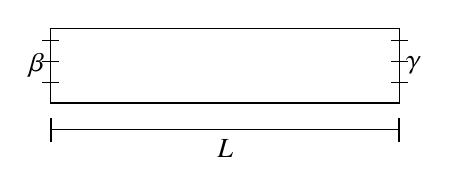
\begin{tikzpicture}[x=0.75pt,y=0.75pt,yscale=-1,xscale=1]
%uncomment if require: \path (0,300); %set diagram left start at 0, and has height of 300

%Shape: Rectangle [id:dp4491854458587017] 
\draw   (141,171) -- (309,171) -- (309,207) -- (141,207) -- cycle ;
%Straight Lines [id:da4657254861857001] 
\draw    (141,207) -- (141,171) (137,197) -- (145,197)(137,187) -- (145,187)(137,177) -- (145,177) ;
%Straight Lines [id:da41979119941170473] 
\draw    (309,207) -- (309,171) (305,197) -- (313,197)(305,187) -- (313,187)(305,177) -- (313,177) ;
%Straight Lines [id:da9943853892815062] 
\draw    (141,220) -- (309,220) ;
\draw [shift={(309,220)}, rotate = 180] [color={rgb, 255:red, 0; green, 0; blue, 0 }  ][line width=0.75]    (0,5.59) -- (0,-5.59)   ;
\draw [shift={(141,220)}, rotate = 180] [color={rgb, 255:red, 0; green, 0; blue, 0 }  ][line width=0.75]    (0,5.59) -- (0,-5.59)   ;

% Text Node
\draw (139,189) node [anchor=east] [inner sep=0.75pt]    {$\beta $};
% Text Node
\draw (311,189) node [anchor=west] [inner sep=0.75pt]    {$\gamma $};
% Text Node
\draw (225,223.4) node [anchor=north] [inner sep=0.75pt]    {$L$};


\end{tikzpicture}

\end{center}

\noindent Diffusion Equation: $\dfrac{1}{\alpha^{2}} \dfrac{\partial \psi}{\partial t}=\dfrac{\partial^{2} \psi}{\partial x^{2}}\, ;\quad 0<x<L,\, t>0$\\[-2ex]

\begin{flushleft}
\begin{tabular}{@{}l@{}}
B.C.s: $\psi(0,t)=\beta,\quad \psi(L,t)=\gamma$\\[1ex]
I.C.: $\psi(x,0)=f(x)$
\end{tabular}
\end{flushleft}

Separation of variables won't work. Instead, we use a Slave Function of one variable to turn the B.C.s homogeneous. The motivation for this is that when subtracted from our initial equation $\psi(x,t)$, the Slave Function $\psi_{S}(x)$ will turn what's left $\psi_{T}(x)$ into a PDE with homogenous B.C.s, which can easily be solved. 

We formalize the "Slave Function" as the "Steady-state" behaviour since it has no time dependency, while $\psi_{T}(x)$ models the transient, or time-dependent, behaviour of the PDE. 

Let $\psi(x, t)=\psi_{S}(x)+\psi_{T}(x, t)$

$\psi_{S}(x)=$ Steady-state temperature.

Sub in this into the PDE:

$\psi_{T}(x, t)=$ Transient temperature.

$$
0+\dfrac{1}{\alpha^{2}} \cdot \dfrac{\partial \psi_{T}}{\partial t}=\dfrac{\partial^{2} \psi_{S}}{\partial x^{2}}+\dfrac{\partial^{2} \psi_{T}}{\partial x^{2}}
$$

First we determine the slave function according to our BC/ICs. 

For the steady-state part, $\dfrac{\partial^{2} \psi_{S}}{\partial x^{2}}=0 \qquad \therefore \psi_{S}(x)=Ax+B$

$$\therefore \psi_{S}(0)=B=\beta\quad \therefore \psi_{S}(x)=A x+\beta$$

$$
\psi_{S}(L)=A L+B=\gamma \quad \therefore A=\dfrac{\gamma-\beta}{L}
$$

Finally, $\boxed{\psi_{S}(x)=\left(\frac{\gamma-\beta}{L}\right)x+\beta}$

In essence, the slave function $\psi_{S}(x)$ "homogenizes" the boundary conditions for the transient function $\psi_{T}(x)$.

For the transient part, $\dfrac{1}{\alpha^{2}} \dfrac{\partial \psi_{T}}{\partial t}=\dfrac{\partial^{2} \psi_{T}}{\partial x^{2}}$

$\left.\begin{array}{l}
    \psi_{T}(0, t)=\psi(0, t)-\psi_{S}(0)=\beta-\beta=0 \quad \text {  Homogeneous. } \\
    \psi_{T}(L, t)=\psi(L, t)-\psi_{S}(L)=\gamma-\gamma=0 \quad \text { Homogeneous. } 
\end{array}\right\}\quad$ B.C.'s

$$
\psi_{T}(x, 0)=\psi(x, 0)-\psi_{S}(x)
=\underbrace{f(x)-\left[\frac{\gamma-\beta}{L}x+\beta\right]}_{F(x)}
\quad \text{I.C.}
$$

The problem is now like BVP 1a. However, keep in mind that the initial condition has changed (from $f(x)$ to $F(x)$ as defined in the line above).

Solve for $\psi_{T}(x, t)$ and add it to $\psi_{S}(x)$ for the final solution. 

Thus, $\psi(x, t)=\psi_{T}(x, t)+\psi_{S}(x)$

$$
\begin{aligned}
& \psi_{T}(x, t)=\dfrac{2}{L} \sum_{n=1}^{\infty} \int_{0}^{L} F(\xi) \sin\left(\dfrac{n \pi \xi}{L}\right)d\xi\, \sin\left(\dfrac{n \pi x}{L}\right)e^{\frac{-\alpha^{2}n^{2}\pi^{2}}{L^{2}}t} \\
& =\int_{0}^{L} G(x, t,\,\xi) F(\xi)d\xi\, ,\quad G(x, t, \xi)=\dfrac{2}{L} \sum_{n=1}^{\infty} \sin\left(\dfrac{n \pi \xi}{L}\right) \sin\left(\dfrac{n \pi x}{L}\right)e^{\frac{-\alpha^{2}n^{2}\pi^{2}}{L^{2}}t}\quad \text{(Green's Function).}
\end{aligned}
$$


\subsection{BVP 5b: Heat Generation/Absorption in a Thin Bar}

This is BVP 1, but with nonzero $Q$.

$$
\dfrac{1}{\alpha^{2}} \cdot \dfrac{\partial \psi}{\partial t}-\nabla^{2} \psi=\dfrac{Q}{K}
$$

Eg.

$$
2 \dfrac{\partial \psi}{\partial t}-\dfrac{\partial^{2} \psi}{\partial x^{2}}=-6 x,\qquad
\begin{aligned}
& \psi(0, t)=3 \quad \psi(x, 0)=x^{3}+2 x+3 \\
& \psi(2, t)=9
\end{aligned}
$$

Let $\psi(x, t)=\psi_{S}(x)+\Phi(x, t) \quad\left(\psi_{T}(x, t)=\Phi(x, t)\right) \quad$ Sub in:

$$
0+2 \dfrac{\partial \Phi}{\partial t}-\dfrac{d^{2} \psi_{S}}{d x^{2}}-\dfrac{\partial^{2} \Phi}{\partial x^{2}}=-6 x
$$

For the slave function $\left(\psi_{S}(x)\right)$, it is in steady state, so $\dfrac{\partial \psi_{S}}{\partial t}=0$

$$\therefore \dfrac{1}{\alpha^{2}}\cdot \dfrac{\partial \psi_{S}}{\partial t}-\nabla^{2} \psi_{S}=\frac{Q}{K} \quad \text { (which is 1 dimensional).}$$

$$-\dfrac{d^{2} \psi_{S}}{d x^{2}}=- 6 x\quad \Rightarrow\quad \psi_{S}(x)=x^{3}+C_{1} x+C_{2} \quad \text { Solve for $C_1,C_2$  using B.C.'s}$$


$$\psi_{S}(0)=C_{2}=3 . \quad \psi_{S}(x)=x^{3}+C_{1} x+3$$

$$\psi_{5}(2)=8+2 C_{1} x+3=9, \quad \therefore C_{1}=-1$$

$$
\therefore \psi_{S}(x)=x^{3}-x+3
$$

Now, address $\Phi(x, t)$ :

$$
\left.\begin{array}{rl}
\text { B.C.'s: } & \Phi(0, t)=\psi(0, t)-\psi_{S}(0)=3-3=0 \\
& \Phi(2, t)=\psi(2, t)-\psi_{S}(2)=9-9=0 \\
\text { I.C: } & \Phi(x, 0)=\left[x^{3}+2 x+3\right]-\left[x^{3}-x+3\right]=3 x
\end{array}\right\} \text{BVP 1a}
$$

$$
\Phi(x, t)=\sum\limits_{n=1}^{\infty} C_{n} \sin \left(\dfrac{n \pi x}{2}\right)e^{\frac{-n^{2} \pi^{2}}{8} t}\quad
$$

$\Phi(x, 0)=\sum\limits_{n=1}^{\infty} C_{n} \sin \left(\dfrac{n \pi x}{2}\right)=3 x \quad$ Fourier Sine Series to resolve IC.

$C_{n}=\dfrac{2}{L}\displaystyle\int_0^L \sin \left(\dfrac{n \pi x}{L}\right) f(x) d x=\dfrac{2}{2} \displaystyle\int_{0}^{2} 3 x \sin \left(\dfrac{n \pi x}{2}\right) d x=\dfrac{-12(-1)^{n}}{n \pi}\quad \text { (Integrate by parts). }$

$$
\therefore \psi(x, t)=\psi_{S}(x)+\Phi(x, t)=x^{3}-x+3-\dfrac{12}{\pi} \sum\limits_{n=1}^{\infty} \dfrac{(-1)^{n}}{n} \sin \left(\dfrac{n \pi x}{2}\right) e^{\frac{-n^{2} \pi^{2}}{8} t}
$$

Physically: $\psi(x, t)$ represents the temperature at a thin rod of length 3, insulated on the sides, initial temperature is $x^{2}+2 x+3$. \quad($Q=$ rate of heat absorption/generation). Diffusivity $\left(\alpha^{2}\right)=\dfrac{1}{2}$. $\dfrac{Q(x)}{k}=-6 x \quad \therefore Q(x)=-6 x k$

\subsection{BVP 5c: Vibrating String with Gravity}

We have $a^{2} \dfrac{\partial^{2} \psi}{\partial x^{2}}-\dfrac{\partial^{2} \psi}{\partial t^{2}}=g$ 

\begin{center}
    

\tikzset{every picture/.style={line width=0.75pt}} %set default line width to 0.75pt        

\begin{tikzpicture}[x=0.75pt,y=0.75pt,yscale=-1,xscale=1]
%uncomment if require: \path (0,300); %set diagram left start at 0, and has height of 300

%Straight Lines [id:da4657254861857001] 
\draw    (141,220) -- (141,196) ;
\draw [shift={(141,196)}, rotate = 90] [color={rgb, 255:red, 0; green, 0; blue, 0 }  ][line width=0.75]    (0,5.59) -- (0,-5.59)   ;
\draw [shift={(141,220)}, rotate = 90] [color={rgb, 255:red, 0; green, 0; blue, 0 }  ][line width=0.75]    (0,5.59) -- (0,-5.59)   ;
%Straight Lines [id:da9943853892815062] 
\draw    (141,220) -- (309,220) ;
%Straight Lines [id:da804925969720879] 
\draw    (309,244) -- (309,220) ;
\draw [shift={(309,220)}, rotate = 90] [color={rgb, 255:red, 0; green, 0; blue, 0 }  ][line width=0.75]    (0,5.59) -- (0,-5.59)   ;
\draw [shift={(309,244)}, rotate = 90] [color={rgb, 255:red, 0; green, 0; blue, 0 }  ][line width=0.75]    (0,5.59) -- (0,-5.59)   ;
%Curve Lines [id:da17066258540314805] 
\draw    (141,196) .. controls (159.2,182.35) and (182.34,206.25) .. (209,222) .. controls (235.66,237.75) and (239,227) .. (249,230) .. controls (259,233) and (276.25,233.83) .. (281,235) .. controls (285.75,236.17) and (301.13,249.9) .. (309,244) ;

% Text Node
\draw (136,208) node [anchor=east] [inner sep=0.75pt]    {$\beta $};
% Text Node
\draw (315,232) node [anchor=west] [inner sep=0.75pt]    {$\gamma $};


\end{tikzpicture}

\end{center}

Ends fixed at $\beta$ and $\gamma$.

B.C.'s: $\psi(0, t)=\beta,\quad \psi(L, t)=\gamma$.

I.C.'s: $\psi(x, 0)=f(x),\quad \psi_{t}(x, 0)=g(x)$.


Use Slave Function

Let $\psi(x, t)=\psi_{S}(x)+\Phi(x, t)$

Substitute into PDE:

$$
a^{2} \dfrac{d^{2} \psi_{S}}{d x^{2}}+\underbrace{a^{2} \dfrac{\partial^{2} \Phi}{\partial x^{2}}- \dfrac{\partial^{2} \Phi}{\partial t^{2}}}_{\text{= 0}}=g
$$

Note that we group our terms such that the transient component is homogeneous. In essence, we split up our inhomogeneous PDE into two: an inhomogeneous ODE $\psi_{S}(x)$ and a homogeneous PDE $\Phi(x,t)$, both of which are solvable. 

$a^{2} \dfrac{d^{2} \psi}{d x^{2}}=g \quad \psi_{S}(0)=\beta, \quad \psi_{S}(L)=\gamma \quad$ Integrate twice

\[
\boxed{
\psi_{S}(x)=-\frac{g x}{2a^{2}}(L-x)+\left(\frac{\gamma-\beta}{L}\right)x+\beta
}
\quad \text{Can be considered the static/equilibrium deflection of the string.}
\]


Once again, we are left with:

$$a^{2} \dfrac{\partial^{2} \Phi}{\partial x^{2}}-\dfrac{\partial^{2} \Phi}{\partial t^{2}}  =0$$

$\left.\begin{array}{ll}
    \text{B.C.'s}: & \Phi(0, t)  =\psi(0, t)-\psi_{S}(0)=\beta-\beta=0 \\
     & \Phi(L, t) =\psi(0, t)-\psi_{S}(0)=\gamma-\gamma=0\\
     \text{I.C.'s}: & \Phi(x, 0)=\psi(x, 0)-\psi_{S}(x)=f(x)-\left\{\dfrac{-g x}{2 a^{2}}(L-x)+\left(\dfrac{\gamma-\beta}{L}\right) x+\beta\right\}=F(x)\\
     & \Phi_{t}(x, 0)=\psi_{t}(x, 0)=g(x)=G(x)
\end{array}\right\}\quad \text{BVP 2}$

As before, sum up $\psi_{S}(x)$ and $\Phi(x,t)$ to obtain $\psi(x,t)$.

\section{BVP 6: Time-Dependent Non-Homogenous Aspects}

\subsection{BVP 6a: Generalized Diffusion, ends at $0^{\circ}$}

General Diffusion Equation: $\dfrac{1}{\alpha^{2}} \dfrac{\partial \psi}{\partial t}-\dfrac{\partial^{2} \psi}{\partial x^{2}}=\parrow{\dfrac{Q(x, t)}{k}}{$\begin{array}{lll}
    \text{In} & \text{BVP 1:} & Q=0 \\
     & \text{BVP 5b:} & Q=f(x)\\
     & \text{BVP 6a:} & Q=f(x,t)
\end{array}$}=h(x, t)$


For simplicity, take $\alpha^{2}=1,\ L=\pi$ (but this can easily be generalized).

Assume ends are maintained at $0^{\circ}$.

$$\therefore \dfrac{\partial \psi}{\partial t}-\dfrac{\partial^{2} \psi}{\partial x^{2}}=h(x, t);\quad 0<x<\pi,\quad t>0$$

\begin{flushleft}
\begin{tabular}{@{}l@{}}
B.C.s: $\psi(0,t)=0,\quad \psi(L,t)=0$\\[1ex]
I.C.: $\psi(x,0)=f(x)$
\end{tabular}
\end{flushleft}


We know the solution for the homogeneous one:

$\psi_{\text {HOM }}(x, t)=\sum\limits_{n=1}^{\infty} C_{n} \sin (n x) e^{-n^{2} t}$ \quad (Complimentary solution).

We can solve with ``Variation of Parameters''.

$$
\text{Let } \boxed{\psi(x, t)=\sum_{n=1}^{\infty} C_{n}(t) \sin (n x)} \text{ *}
$$

(Spatial part satisfies the B.C.'s, so the $e^{-n^{2} t}$ gets incorporated into $C_{n}(t)$.)

Physically, $e^{-n^{2} t}$ represented the decrease with time from an initial temperature of $f(x)$ to O (because there is no heat generation or absorption). However, this term is pointless with nonzero heat generation/absorption.

Sub * into the PDE:

$\sum\limits_{n=1}^{\infty}\left[\dfrac{d C_{n}}{d t}+n^{2} C_{n}\right] \sin (n x)=h(x, t)$ \quad Apply the Fourier Sine trick (all 0 unless $n=k$).

$$
\begin{aligned}
& \sum_{n=1}^{\infty}\left[\frac{d C_{n}}{d t}+n^{2} C_{n}\right] \int_{0}^{\pi} \underbrace{\sin(k x) \sin(n x)\, dx}_{\delta_{k,x}\cdot \frac{\pi}{2}} = \int_{0}^{\pi} \sin(k x) h(x,t)\, dx \\
& \frac{\pi}{2}\left[\frac{d C_{k}}{d t}+k^{2} C_{k}\right]= \int_{0}^{\pi} \sin(k x) h(x,t)\, dx \quad (n=k) \\
& \frac{d C_{n}}{d t}+n^{2} C_{n} = \frac{2}{\pi} \int_{0}^{\pi} \sin(n x) h(x,t)\, dx = B_{n}(t)
\end{aligned}
$$

This is a first-order linear ODE (we solve it by multiplying each side with an integrating factor $\mu(t)$):

$$
\begin{aligned}
& \frac{d C_n}{dt} + \underbrace{n^2 C_n}_{p(t)} = \underbrace{B_n(t)}_{g(t)} \quad \mu(t)= e^{\int p(t)\, dt} = e^{n^2 t} \\
& \underbrace{\frac{d C_n}{dt}\, e^{n^2 t} + n^2 C_n\, e^{n^2 t}}_{\text{reverse prod. rule}} = B_n(t)\, e^{n^2 t}
\end{aligned}
$$


$\dfrac{d}{d t}\left[C_{n} e^{n^{2}t}\right]=B_{n}(t) e^{n^{2} t}$

$\displaystyle\int_{0}^{t} \dfrac{d}{d \tau}\left[C_{n} e^{n^{2} \tau}\right] d \tau=\displaystyle\int_{0}^{t} B_{n}(\tau) e^{n^{2} \tau} d \tau$

$e^{-n^{2}t}\left[C_{n}(t) e^{n^{2} t}-C_{n}(0)\right]=\displaystyle\int_{0}^{t} B_{n}(\tau) e^{n^{2} \tau} d \tau$

$$
\boxed{C_{n}(t)=C_{n}(0) e^{-n^{2} t}+e^{-n^{2} t} \displaystyle\int_{0}^{t} B_{n}(\tau) e^{n^{2} \tau} d \tau}
$$

From the IC: $\psi(x, 0)=\sum\limits_{n=1}^{\infty} C_{n}(0) \sin (n x)=f(x)$

$$
\therefore \boxed{C_{n}(0)=\dfrac{2}{\pi} \displaystyle\int_{0}^{\pi} f(\xi) \sin (n\xi) d\xi}
$$

Plug $C_{n}(t)$ and $C_{n}(0)$ into the (boxed) general solution. $\tau$ and $\xi$ are just dummy variables.

\subsection{BVP 6b. Generalized Diffusion. Dirichlet, B.C. function of time}

\begin{center}
    

\tikzset{every picture/.style={line width=0.75pt}} %set default line width to 0.75pt        

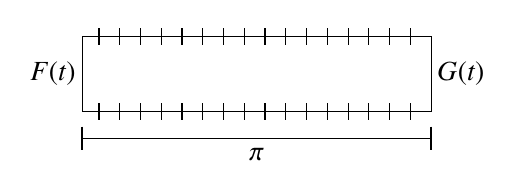
\begin{tikzpicture}[x=0.75pt,y=0.75pt,yscale=-1,xscale=1]
%uncomment if require: \path (0,300); %set diagram left start at 0, and has height of 300

%Shape: Rectangle [id:dp4491854458587017] 
\draw   (141,171) -- (309,171) -- (309,207) -- (141,207) -- cycle ;
%Straight Lines [id:da4657254861857001] 
\draw    (309,171) -- (141,171) (299,175) -- (299,167)(289,175) -- (289,167)(279,175) -- (279,167)(269,175) -- (269,167)(259,175) -- (259,167)(249,175) -- (249,167)(239,175) -- (239,167)(229,175) -- (229,167)(219,175) -- (219,167)(209,175) -- (209,167)(199,175) -- (199,167)(189,175) -- (189,167)(179,175) -- (179,167)(169,175) -- (169,167)(159,175) -- (159,167)(149,175) -- (149,167) ;
%Straight Lines [id:da41979119941170473] 
\draw    (309,207) -- (141,207) (299,211) -- (299,203)(289,211) -- (289,203)(279,211) -- (279,203)(269,211) -- (269,203)(259,211) -- (259,203)(249,211) -- (249,203)(239,211) -- (239,203)(229,211) -- (229,203)(219,211) -- (219,203)(209,211) -- (209,203)(199,211) -- (199,203)(189,211) -- (189,203)(179,211) -- (179,203)(169,211) -- (169,203)(159,211) -- (159,203)(149,211) -- (149,203) ;
%Straight Lines [id:da9943853892815062] 
\draw    (141,220) -- (309,220) ;
\draw [shift={(309,220)}, rotate = 180] [color={rgb, 255:red, 0; green, 0; blue, 0 }  ][line width=0.75]    (0,5.59) -- (0,-5.59)   ;
\draw [shift={(141,220)}, rotate = 180] [color={rgb, 255:red, 0; green, 0; blue, 0 }  ][line width=0.75]    (0,5.59) -- (0,-5.59)   ;

% Text Node
\draw (139,189) node [anchor=east] [inner sep=0.75pt]    {$F( t)$};
% Text Node
\draw (311,189) node [anchor=west] [inner sep=0.75pt]    {$G( t)$};
% Text Node
\draw (225,223.4) node [anchor=north] [inner sep=0.75pt]    {$\pi $};


\end{tikzpicture}

\end{center}

$$\dfrac{\partial\psi}{\partial t}-\dfrac{\partial^2\psi}{\partial t^2}=h(x,t)\qquad \begin{array}{l}
     \psi(0,t)=F(t)  \\
     \psi(\pi,t)=G(t) 
\end{array}\qquad \psi(x,0)=f(t)$$

Now we use a Slave Function of 2 variables. (since the B.C.s are both nonhomogenous and a function of time). Here, the slave function once again represents the long-term behaviour of the system, but this isn't time-indepdent; it just means that the transient components decays relative to the non-constant slave function.

$$\psi(x, t)=\psi_{S}(x, t)+\Phi(x, t)$$

In BVP 5a, we had $\psi(0, t)=\beta,\ \psi(L, t)=\gamma$ with $\psi_{S}(x)=A x+B$.

With the time-variant component, we have:

$$
\psi_{S}(x, t)=A(t) x+B(t)
$$

Thus. $\psi_{S}(0, t)=B(t)$

$\therefore \psi_{S}(x,t)=A(t) x+F(t) \quad$ Now, we incorporate the other B.C.

$\psi_{S}(\pi, t)=A(t) \parrow{\pi}{or generally, $L$}+F(t)=G(t)$

$$
\therefore \boxed{\psi_{S}(x, t)=\left[\dfrac{G(t)-F(t)}{\pi}\right] x+F(t)}
$$

Sub in $\psi(x, t)=\psi_{S}(x, t)+\Phi(x, t)$ into PDE $\dfrac{\partial \psi}{\partial t}-\dfrac{\partial^{2} \psi}{\partial x^{2}}=h(x, t)$.

$$
\therefore\left\{\left[\dfrac{G^{\prime}(t)-F^{\prime}(t)}{\pi}\right] x+F^{\prime}(t)-0\right\}+\dfrac{\partial \Phi}{\partial t}-\dfrac{\partial^{2} \Phi}{\partial x^{2}}+0=h(x, t)
$$

Moving everything to the RHS, we have:

\[
\begin{aligned}
\frac{\partial \Phi}{\partial t} - \frac{\partial^2 \Phi}{\partial x^2} 
&= h(x,t) - \Biggl\{ \left[\frac{G'(t)-F'(t)}{\pi}\right] x + F'(t) \Biggr\}, \\[1ex]
\text{B.C.'s:}\quad \Phi(0,t) 
&= \psi(0,t) - \psi_S(0,t) = F(t) - F(t) = 0, \\[1ex]
\Phi(\pi,t) 
&= \psi(\pi,t) - \psi_S(\pi,t) = G(t) - G(t) = 0, \\[1ex]
\text{I.C.:}\quad \Phi(x,0) 
&= \psi(x,0) - \psi_s(x,0) \\
&= f(x) - \Biggl\{ \left[\frac{G(0)-F(0)}{\pi}\right] x + F(0) \Biggr\} \\
&= \mathcal{F}(x)
\end{aligned}
\]

\begin{flushleft}
As we can see, the PDE of $\Phi(x,t)$ has reduced to an inhomogeneous, time dependent PDE with homogenous B.C.s. This is simply BVP 6a, and we can solve for $\Phi(x,t)$ as we did BVP 6a.

Finally, don't forget to add the slave function to your solution $\psi(x,t)=\Phi(x,t)+\psi_s(x,t)$
\end{flushleft}

\subsection{BVP 6c. Generalized Diffusion. Neumann, B.C. function of time}

\begin{center}
    

\tikzset{every picture/.style={line width=0.75pt}} %set default line width to 0.75pt        

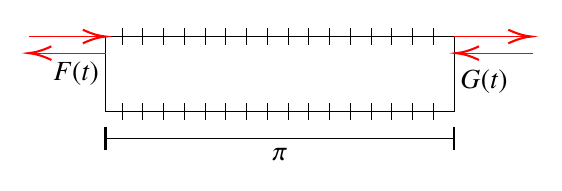
\begin{tikzpicture}[x=0.75pt,y=0.75pt,yscale=-1,xscale=1]
%uncomment if require: \path (0,300); %set diagram left start at 0, and has height of 300

%Shape: Rectangle [id:dp4491854458587017] 
\draw   (141,171) -- (309,171) -- (309,207) -- (141,207) -- cycle ;
%Straight Lines [id:da4657254861857001] 
\draw    (309,171) -- (141,171) (299,175) -- (299,167)(289,175) -- (289,167)(279,175) -- (279,167)(269,175) -- (269,167)(259,175) -- (259,167)(249,175) -- (249,167)(239,175) -- (239,167)(229,175) -- (229,167)(219,175) -- (219,167)(209,175) -- (209,167)(199,175) -- (199,167)(189,175) -- (189,167)(179,175) -- (179,167)(169,175) -- (169,167)(159,175) -- (159,167)(149,175) -- (149,167) ;
%Straight Lines [id:da41979119941170473] 
\draw    (309,207) -- (141,207) (299,211) -- (299,203)(289,211) -- (289,203)(279,211) -- (279,203)(269,211) -- (269,203)(259,211) -- (259,203)(249,211) -- (249,203)(239,211) -- (239,203)(229,211) -- (229,203)(219,211) -- (219,203)(209,211) -- (209,203)(199,211) -- (199,203)(189,211) -- (189,203)(179,211) -- (179,203)(169,211) -- (169,203)(159,211) -- (159,203)(149,211) -- (149,203) ;
%Straight Lines [id:da9943853892815062] 
\draw    (141,220) -- (309,220) ;
\draw [shift={(309,220)}, rotate = 180] [color={rgb, 255:red, 0; green, 0; blue, 0 }  ][line width=0.75]    (0,5.59) -- (0,-5.59)   ;
\draw [shift={(141,220)}, rotate = 180] [color={rgb, 255:red, 0; green, 0; blue, 0 }  ][line width=0.75]    (0,5.59) -- (0,-5.59)   ;
%Straight Lines [id:da8560092446071703] 
\draw [color={rgb, 255:red, 255; green, 0; blue, 0 }  ,draw opacity=1 ]   (104,171) -- (139,171) ;
\draw [shift={(141,171)}, rotate = 180] [color={rgb, 255:red, 255; green, 0; blue, 0 }  ,draw opacity=1 ][line width=0.75]    (10.93,-3.29) .. controls (6.95,-1.4) and (3.31,-0.3) .. (0,0) .. controls (3.31,0.3) and (6.95,1.4) .. (10.93,3.29)   ;
%Straight Lines [id:da2853108945261318] 
\draw [color={rgb, 255:red, 255; green, 0; blue, 0 }  ,draw opacity=1 ]   (106,179) -- (141,179) ;
\draw [shift={(104,179)}, rotate = 0] [color={rgb, 255:red, 255; green, 0; blue, 0 }  ,draw opacity=1 ][line width=0.75]    (10.93,-3.29) .. controls (6.95,-1.4) and (3.31,-0.3) .. (0,0) .. controls (3.31,0.3) and (6.95,1.4) .. (10.93,3.29)   ;
%Straight Lines [id:da5500015788543415] 
\draw [color={rgb, 255:red, 255; green, 0; blue, 0 }  ,draw opacity=1 ]   (309,171) -- (344,171) ;
\draw [shift={(346,171)}, rotate = 180] [color={rgb, 255:red, 255; green, 0; blue, 0 }  ,draw opacity=1 ][line width=0.75]    (10.93,-3.29) .. controls (6.95,-1.4) and (3.31,-0.3) .. (0,0) .. controls (3.31,0.3) and (6.95,1.4) .. (10.93,3.29)   ;
%Straight Lines [id:da9408208078727294] 
\draw [color={rgb, 255:red, 255; green, 0; blue, 0 }  ,draw opacity=1 ]   (312,179) -- (347,179) ;
\draw [shift={(310,179)}, rotate = 0] [color={rgb, 255:red, 255; green, 0; blue, 0 }  ,draw opacity=1 ][line width=0.75]    (10.93,-3.29) .. controls (6.95,-1.4) and (3.31,-0.3) .. (0,0) .. controls (3.31,0.3) and (6.95,1.4) .. (10.93,3.29)   ;

% Text Node
\draw (139,189) node [anchor=east] [inner sep=0.75pt]    {$F( t)$};
% Text Node
\draw (311,193) node [anchor=west] [inner sep=0.75pt]    {$G( t)$};
% Text Node
\draw (225,223.4) node [anchor=north] [inner sep=0.75pt]    {$\pi $};


\end{tikzpicture}

\end{center}

$$\dfrac{\partial \psi}{\partial t}-\dfrac{\partial^2\psi}{\partial x^2}=h(x,t)\qquad \begin{array}{ll}
     \psi_{x}(0, t)=F(t) & \psi(x, 0)=f(t) \\
     \psi_{x}(\pi, t)=G(t) & 
\end{array}$$

Rate of heat inflow (outflow) at ends represented by $F(x), G(x)$.

Same process, assume the general solution is equal to the sum of a transient function and slave function.

$$
\psi(x, t)=\psi_{S}(x, t)+\Phi(x, t)
$$


$\therefore \dfrac{\partial \psi_{S}}{\partial x}=A(t)$. This slave function can't satisfy two derivative-level (Neumann) B.C.s, so we go "up a power".

$\therefore \psi_{S}(x, t)=A(t) x^{2}+B(t) x$

$\therefore \dfrac{\partial \psi_{S}}{\partial x}=2 A(t) x+B(t) \quad \text { Apply B.C.'s: }$

$$
\begin{aligned}
& \left.\dfrac{\partial \psi_{S}}{\partial x}\right|_{x=0}=B(t)=F(t) \\
& \left.\dfrac{\partial \psi_{S}}{\partial x}\right|_{x=\pi}=2 \pi A(t)+F(t)=G(t) \qquad \therefore A(t)=\dfrac{G(t)-F(t)}{2 \pi} 
\end{aligned}
$$

$\therefore \boxed{\psi_{S}(x, t)=\left[\dfrac{G(t)-F(t)}{2 \pi}\right] x^{2}+F(t) x}$

Sub in $\psi(x, t)=\left[\dfrac{G(t)-F(t)}{2 \pi}\right] x^{2}+F(t) x+\Phi(x, t)$ into the PDE:

$$
\begin{aligned}
& \left\{\left[\dfrac{G^{\prime}(t)-F^{\prime}(t)}{2 \pi}\right] x^{2}+F^{\prime}(t) x-\left[\dfrac{G(t)-F(t)}{\pi}\right]\right\}+\dfrac{\partial \Phi}{\partial t}-\dfrac{\partial^{2} \Phi}{\partial x^{2}}=h(x, t) \\
& \dfrac{\partial \Phi}{\partial t}-\dfrac{\partial^{2} \Phi}{\partial x^{2}}=h(x, t)-\left\{\left[\dfrac{G^{\prime}(t)-F^{\prime}(t)}{2 \pi}\right] x^{2}+F^{\prime}(t) x-\left[\dfrac{G(t)-F(t)}{\pi}\right]\right\}=\mathcal{H}(x, t)
\end{aligned}
$$

All that happened was that the RHS of the transient function $\Phi(x,t)$ got modified. In turn, its B.C.s will become homogenous, allowing us to solve for it. We did the same thing in BVP 6b.  

Apply B.C.'s on $\Phi(x, t)$:

$$
\begin{aligned}
& \Phi_{x}(0, t)=\psi_{x}(0, t)-\dfrac{\partial \psi_{S}}{\partial x}(0, t)=F(t)-F(t)=0 \\
& \Phi_{x}(\pi, t)=\psi_{x}(\pi, t)-\dfrac{\partial \psi_{S}}{\partial x}(\pi, t)=G(t)-G(t)=0
\end{aligned}
$$

I.C: $\Phi(x, 0)=\psi(x, 0)-\psi_{S}(x, 0)=f(x)-\left\{\left[\dfrac{G(0)-F(0)}{2 \pi}\right] x^{2}+F(0) x\right\}=\mathcal{F}(x, t)$

Once again. this reduces to BVP 6a. However, with Neumann B.C.s instead of Dirichlet.

With the same reasoning in BVP 6a, we let: 

$$
\Phi(x, t)=\sum\limits_{n=0}^{\infty} C_{n}(t) \cos (n x)=C_{0}(t)+\sum\limits_{n=1}^{\infty} C_{n}(t) \cos (n x)
$$

Sub into PDE:

$\left[\dfrac{d C_{0}}{d t}\right] \cdot 1+\sum\limits_{n=1}^{\infty}\left[\dfrac{d C_{n}}{d t}+n^{2} C_{n}\right] \cos (n x)=\mathcal{H}(x, t) \quad$ Apply Fourier Cosine trick

$$
\begin{aligned}
& \therefore \dfrac{d C_{0}}{d t}=\dfrac{1}{\pi}\int_{0}^{\pi} \mathcal{H}(x,t)\,dx = B_{0}(t) \\
& \therefore \boxed{C_{0}(t)=C_{0}(0)+\int_{0}^{t} B_{0}(\tau)\,d\tau} \\
& \therefore \dfrac{d C_{n}}{d t}+n^{2} C_{n}=\dfrac{2}{\pi}\int_{0}^{\pi} \mathcal{H}(x,t)\cos(nx)\,dx = B_{n}(t)
\end{aligned}
$$

Like in BVP 6a, apply an integrating factor of \(e^{-n^{2}t}\) to get:

$$
\boxed{C_{n}(t)=C_{n}(0)e^{-n^{2}t}+e^{-n^{2}t}\int_{0}^{t} e^{n^{2}\tau} B_{n}(\tau)\,d\tau}
$$

Finally, since
\[
\Phi(x, 0)=C_{0}(0)+\sum_{n=1}^{\infty} C_{n}(0) \cos(nx)=\mathcal{F}(x)
\quad \text{(Fourier Cosine Series)},
\]
we have

$$
\begin{aligned}
& \boxed{C_{0}(0)=\dfrac{1}{\pi}\int_{0}^{\pi} \mathcal{F}(\xi)\,d\xi} \\
& \boxed{C_{n}(0)=\dfrac{2}{\pi}\int_{0}^{\pi} \mathcal{F}(\xi)\cos(n\xi)\,d\xi}
\end{aligned}
$$

Plug and solve for $\Phi(x, t)$. Note that the use of $\tau$ and $\xi$ as variables is just to prevent ambiguity with the $t$ on the bounds of the integrals. Once all computations are done, all these functions are functions of time, $t$.

\section{BVP 7: 3-Variable Diffusion}

Analagous to BVP 3, but not steady state $\left(\dfrac{\partial \psi}{\partial t} \neq 0\right)$

So the temperature is $\psi(x, y, t)$ at any point $P(x, y)$

Assume $\alpha^{2}=1,\ L=\pi$ for simplicity.

\begin{center}
    

\tikzset{every picture/.style={line width=0.75pt}} %set default line width to 0.75pt        

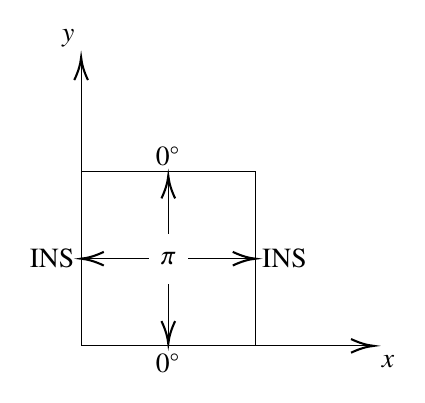
\begin{tikzpicture}[x=0.75pt,y=0.75pt,yscale=-1,xscale=1]
%uncomment if require: \path (0,300); %set diagram left start at 0, and has height of 300

%Shape: Square [id:dp5817550274120495] 
\draw   (100,130) -- (184,130) -- (184,214) -- (100,214) -- cycle ;
%Straight Lines [id:da738039226905576] 
\draw    (100,214) -- (239,214) ;
\draw [shift={(241,214)}, rotate = 180] [color={rgb, 255:red, 0; green, 0; blue, 0 }  ][line width=0.75]    (10.93,-3.29) .. controls (6.95,-1.4) and (3.31,-0.3) .. (0,0) .. controls (3.31,0.3) and (6.95,1.4) .. (10.93,3.29)   ;
%Straight Lines [id:da18159895323009168] 
\draw    (100,214) -- (100,77) ;
\draw [shift={(100,75)}, rotate = 90] [color={rgb, 255:red, 0; green, 0; blue, 0 }  ][line width=0.75]    (10.93,-3.29) .. controls (6.95,-1.4) and (3.31,-0.3) .. (0,0) .. controls (3.31,0.3) and (6.95,1.4) .. (10.93,3.29)   ;
%Straight Lines [id:da5386843576419114] 
\draw    (102,172) -- (182,172) ;
\draw [shift={(184,172)}, rotate = 180] [color={rgb, 255:red, 0; green, 0; blue, 0 }  ][line width=0.75]    (10.93,-3.29) .. controls (6.95,-1.4) and (3.31,-0.3) .. (0,0) .. controls (3.31,0.3) and (6.95,1.4) .. (10.93,3.29)   ;
\draw [shift={(100,172)}, rotate = 0] [color={rgb, 255:red, 0; green, 0; blue, 0 }  ][line width=0.75]    (10.93,-3.29) .. controls (6.95,-1.4) and (3.31,-0.3) .. (0,0) .. controls (3.31,0.3) and (6.95,1.4) .. (10.93,3.29)   ;
%Straight Lines [id:da27606858564834513] 
\draw    (142,211) -- (142,134) ;
\draw [shift={(142,132)}, rotate = 90] [color={rgb, 255:red, 0; green, 0; blue, 0 }  ][line width=0.75]    (10.93,-3.29) .. controls (6.95,-1.4) and (3.31,-0.3) .. (0,0) .. controls (3.31,0.3) and (6.95,1.4) .. (10.93,3.29)   ;
\draw [shift={(142,213)}, rotate = 270] [color={rgb, 255:red, 0; green, 0; blue, 0 }  ][line width=0.75]    (10.93,-3.29) .. controls (6.95,-1.4) and (3.31,-0.3) .. (0,0) .. controls (3.31,0.3) and (6.95,1.4) .. (10.93,3.29)   ;

% Text Node
\draw  [draw opacity=0][fill={rgb, 255:red, 255; green, 255; blue, 255 }  ,fill opacity=1 ]  (132.5,160) -- (151.5,160) -- (151.5,184) -- (132.5,184) -- cycle  ;
\draw (142,172) node    {$\pi $};
% Text Node
\draw (98,71.6) node [anchor=south east] [inner sep=0.75pt]    {$y$};
% Text Node
\draw (243,217.4) node [anchor=north west][inner sep=0.75pt]    {$x$};
% Text Node
\draw (186,172) node [anchor=west] [inner sep=0.75pt]   [align=left] {INS};
% Text Node
\draw (98,172) node [anchor=east] [inner sep=0.75pt]   [align=left] {INS};
% Text Node
\draw (142,128.6) node [anchor=south] [inner sep=0.75pt]    {$0^{\circ }$};
% Text Node
\draw (142,216.4) node [anchor=north] [inner sep=0.75pt]    {$0^{\circ }$};


\end{tikzpicture}

\end{center}

$$
\dfrac{\partial \psi}{\partial t}=\dfrac{\partial^{2} \psi}{\partial x^{2}}+\dfrac{\partial^{2} \psi}{\partial y^{2}}\quad 
\begin{array}[c]{l}
     0<x<\pi \\
     0<y<\pi 
\end{array}\quad 
\underbrace{
\begin{array}[c]{l}
     \psi_x(0,y,t)=0\\
     \psi(\pi,y,t)=0 
\end{array}
}_{\text{2 x Neumann}}\quad 
\underbrace{
\begin{array}[c]{l}
     \psi(x,0,t)=0\\
     \psi(x,\pi,t)=0 
\end{array}
}_{\text{2 x Dirichlet}}\quad \psi(x,y,0)=f(x,y)
$$


Separation of Variables:

$$
\begin{aligned}
& \psi(x, y, t)=X(x) Y(y) T(t)=0 \\
& \begin{array}{ll}
    X^{\prime}(0)=0 & Y(0)=0 \\
    X^{\prime}(\pi)=0 & Y(\pi)=0 
\end{array}
\end{aligned}
$$

$\left\{X Y \dfrac{d T}{d t}=\dfrac{d^{2} X}{d x^{2}} Y T+X \dfrac{d^{2} Y}{d y^{2}} T\right\} \cdot \dfrac{1}{X Y T}$

$\dfrac{1}{T} \dfrac{d T}{d t}=\dfrac{1}{X} \dfrac{d^{2} X}{d x^{2}}+\dfrac{1}{Y} \dfrac{d^{2} Y}{d y^{2}}$

$\dfrac{1}{T} \dfrac{d T}{d t}-\dfrac{1}{Y} \dfrac{d^{2} Y}{d y^{2}}=\dfrac{1}{X} \dfrac{d^{2} X}{d x^{2}}=\text { constant. }=\lambda$

$\dfrac{1}{X} \dfrac{d^{2} X}{d x^{2}}=\lambda,\quad X^{\prime}(0)=0,\ X^{\prime}(\pi)=0\quad \text{BVP 1b}$

$$
\therefore X(x)=A_{n} \cos \left(\frac{n \pi x}{\pi}\right)
=A_{n} \cos (n x),\quad n=0,1,\ldots \qquad \lambda=\frac{n^{2}\pi^{2}}{\pi^{2}}=n^{2}
$$

Now we are left with:

$\dfrac{1}{T} \cdot \dfrac{d T}{d t}-\dfrac{1}{Y} \dfrac{d^{2} Y}{d y^{2}}=\lambda=-n^{2}$

$$\therefore \dfrac{1}{T} \cdot \dfrac{d T}{d t}+n^{2}=\dfrac{1}{Y} \dfrac{d^{2} Y}{d y^{2}}=\text { constant }=\parrow{\mu}{Different from $\lambda$}$$

$\dfrac{d^{2} Y}{d y^{2}}=Y \mu, Y(0)=0, Y(\pi)=0 \quad$ \text{BVP 1a}

$Y(y)=B_{k} \sin (k y), k=1,2,3 \ldots \quad \mu=\parrow{\dfrac{k^{2} \pi^{2}}{\pi^{2}}}{``H''}=k^{\prime 2}$

Finally, $\dfrac{d T}{d t}=T\left(-n^{2}-\mu\right)$

$$
\therefore T(t)=C_{n k} e^{-\left(n^{2}+k^{2}\right) t}
$$

So the complete solution is:

$$
\boxed{\psi_{n k}(x, y, t)=D_{n k} \cos (n x) \sin (k y) e^{-\left(n^{2}+k^{2}\right) t}}
$$

$\cos$ because $x$ B.C.'s are Neumann\\
$\sin$ because $y$ B.C.'s are Dirichlet.

Same Fourier thing as BVP 1, but multivariable:

$$
\left[\dfrac{\partial}{\partial t}-\dfrac{\partial^{2}}{\partial x^{2}}-\dfrac{\partial^{2}}{\partial y^{2}}\right] \psi(x, y, t)=0
$$

$\mathcal{L} \psi=0$. Want nullspace of this linear operator ($\mathcal{L}$ is a linear operator, so we can use superposition)

$$
\therefore \psi(x, y, t)=\sum\limits_{k=1}^{\infty} \sum\limits_{n=0}^{\infty} D_{n k} \cos (n x) \sin (k y) e^{-\left(n^{2}+k^{2}\right) t}
$$

Apply IC, extract $n=0$ term:

$$
\psi(x, y, 0)=\sum\limits_{k=1}^{\infty} D_{0 k} \sin (k y)+\sum\limits_{k=1}^{\infty} \sum\limits_{n=1}^{\infty} D_{n k} \cos (n x) \sin (k y)=f(x, y)
$$

We do the Fourier Sine Trick: (multiply by $\sin(ly)$, take double integral).

$$
\begin{aligned}
& \sum_{k=1}^{\infty} D_{0k} \int_{0}^{\pi} \underbrace{(1)\,dx}_{\pi} \int_{0}^{\pi} \underbrace{\sin(l y)\sin(ky)}_{\delta_{l,k}\cdot \frac{\pi}{2}}\,dy 
+ \sum_{k=1}^{\infty} \sum_{n=1}^{\infty} D_{nk} \int_{0}^{\pi} \underbrace{(1)\cos(nx)\,dx}_{0} \int_{0}^{\pi} \underbrace{\sin(l y)\sin(ky)\,dy}_{\delta_{l,k}\cdot \frac{\pi}{2}}\\[1ex]
&\quad = \int_{0}^{\pi} \int_{0}^{\pi} \sin(l y)f(x,y)\,dx\,dy\quad\text{only nonzero when } l=k,\\[1ex]
& \frac{\pi^2}{2}\, D_{0l} = \int_{0}^{\pi} \int_{0}^{\pi} \sin(l y)f(x,y)\,dx\,dy.
\end{aligned}
$$

$$
\therefore \boxed{D_{0k}=\frac{2}{\pi^{2}} \int_{0}^{\pi} \int_{0}^{\pi} \sin(l y)f(x,y)\,dx\,dy}
$$

Repeat with \(\cos(mx)\sin(ly)\) for \(D_{nk}\) and sub in \(D_{0k}\) and \(D_{nk}\) into the general solution.

$$
\begin{aligned}
& \sum_{k=1}^{\infty} D_{0k} \int_{0}^{\pi} \sin(l y)\sin(ky)\,dy \int_{0}^{\pi} \underbrace{(1)\cos(mx)\,dx}_{0}
+ \sum_{k=1}^{\infty} \sum_{n=1}^{\infty} D_{nk} \int_{0}^{\pi} \underbrace{\cos(mx)\cos(nx)\,dx}_{\frac{\pi}{2}\,\delta_{m,n}} \int_{0}^{\pi} \underbrace{\sin(l y)\sin(ky)\,dy}_{\frac{\pi}{2}\,\delta_{l,k}}\\[1ex]
&\quad = \int_{0}^{\pi} \int_{0}^{\pi} \cos(mx)\sin(ly)f(x,y)\,dx\,dy.
\end{aligned}
$$

$$
\therefore \boxed{D_{nk}=\frac{4}{\pi^{2}} \int_{0}^{\pi} \int_{0}^{\pi} \cos(nx)\sin(ky)f(x,y)\,dx\,dy}
$$

\section{BVP 8: Poisson's Equation}

$$
\nabla^{2} \psi=-F \quad(\text { Poisson's Equation) }
$$

$F$ can represent:

$\psi=$ Velocity Potential, $F=$ Rate of Fluid Generation.\\
$\psi=$ Steady State Temperature, $F=$ Rate of Heat Generation.\\
$\psi=$ Displacement, $F=$ External Force/ mass.\\
$\psi=$ Electric Potential, $F=$ Charge Density.\\
Eg. Steady-State Temp Distribution:

\begin{center}
    

\tikzset{every picture/.style={line width=0.75pt}} %set default line width to 0.75pt        

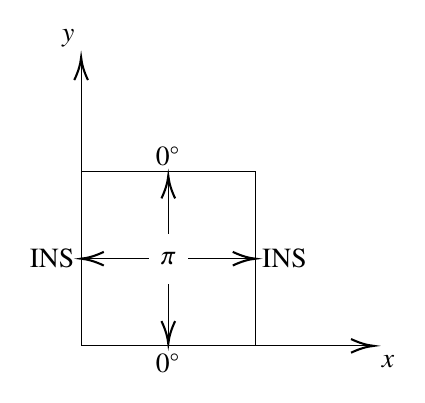
\begin{tikzpicture}[x=0.75pt,y=0.75pt,yscale=-1,xscale=1]
%uncomment if require: \path (0,300); %set diagram left start at 0, and has height of 300

%Shape: Square [id:dp5817550274120495] 
\draw   (100,130) -- (184,130) -- (184,214) -- (100,214) -- cycle ;
%Straight Lines [id:da738039226905576] 
\draw    (100,214) -- (239,214) ;
\draw [shift={(241,214)}, rotate = 180] [color={rgb, 255:red, 0; green, 0; blue, 0 }  ][line width=0.75]    (10.93,-3.29) .. controls (6.95,-1.4) and (3.31,-0.3) .. (0,0) .. controls (3.31,0.3) and (6.95,1.4) .. (10.93,3.29)   ;
%Straight Lines [id:da18159895323009168] 
\draw    (100,214) -- (100,77) ;
\draw [shift={(100,75)}, rotate = 90] [color={rgb, 255:red, 0; green, 0; blue, 0 }  ][line width=0.75]    (10.93,-3.29) .. controls (6.95,-1.4) and (3.31,-0.3) .. (0,0) .. controls (3.31,0.3) and (6.95,1.4) .. (10.93,3.29)   ;
%Straight Lines [id:da5386843576419114] 
\draw    (102,172) -- (182,172) ;
\draw [shift={(184,172)}, rotate = 180] [color={rgb, 255:red, 0; green, 0; blue, 0 }  ][line width=0.75]    (10.93,-3.29) .. controls (6.95,-1.4) and (3.31,-0.3) .. (0,0) .. controls (3.31,0.3) and (6.95,1.4) .. (10.93,3.29)   ;
\draw [shift={(100,172)}, rotate = 0] [color={rgb, 255:red, 0; green, 0; blue, 0 }  ][line width=0.75]    (10.93,-3.29) .. controls (6.95,-1.4) and (3.31,-0.3) .. (0,0) .. controls (3.31,0.3) and (6.95,1.4) .. (10.93,3.29)   ;
%Straight Lines [id:da27606858564834513] 
\draw    (142,211) -- (142,134) ;
\draw [shift={(142,132)}, rotate = 90] [color={rgb, 255:red, 0; green, 0; blue, 0 }  ][line width=0.75]    (10.93,-3.29) .. controls (6.95,-1.4) and (3.31,-0.3) .. (0,0) .. controls (3.31,0.3) and (6.95,1.4) .. (10.93,3.29)   ;
\draw [shift={(142,213)}, rotate = 270] [color={rgb, 255:red, 0; green, 0; blue, 0 }  ][line width=0.75]    (10.93,-3.29) .. controls (6.95,-1.4) and (3.31,-0.3) .. (0,0) .. controls (3.31,0.3) and (6.95,1.4) .. (10.93,3.29)   ;

% Text Node
\draw  [draw opacity=0][fill={rgb, 255:red, 255; green, 255; blue, 255 }  ,fill opacity=1 ]  (132.5,160) -- (151.5,160) -- (151.5,184) -- (132.5,184) -- cycle  ;
\draw (142,172) node    {$\pi $};
% Text Node
\draw (98,71.6) node [anchor=south east] [inner sep=0.75pt]    {$y$};
% Text Node
\draw (243,217.4) node [anchor=north west][inner sep=0.75pt]    {$x$};
% Text Node
\draw (186,172) node [anchor=west] [inner sep=0.75pt]   [align=left] {INS};
% Text Node
\draw (98,172) node [anchor=east] [inner sep=0.75pt]   [align=left] {INS};
% Text Node
\draw (142,128.6) node [anchor=south] [inner sep=0.75pt]    {$0^{\circ }$};
% Text Node
\draw (142,216.4) node [anchor=north] [inner sep=0.75pt]    {$0^{\circ }$};


\end{tikzpicture}

\end{center}

$$\parrow{\nabla^2\psi=-F(x,y)}{$\substack{\text{Unlike BVP 7, PDE is not}\\
\text{homogeneous, but $\frac{\partial\psi}{\partial t}=0$}}$}\qquad \underbrace{\begin{array}[t]{l}
     \psi_x(0,y,t)=0 \\
     \psi_x(\pi,y,t)=0
\end{array}}_{\text{2 x Neumann}} \qquad \underbrace{\begin{array}[t]{l}
     \psi(x,0,t)=0 \\
     \psi(x,\pi,t)=0
\end{array}}_{\text{2 x Dirichlet}}$$

Using the same principle from BVP 7:


\[
\boxed{
\psi(x, y)=\sum_{k=1}^{\infty} \sum_{n=0}^{\infty} C_{nk}\,
\underbrace{\cos (n x)}_{\text{Newman}}\, \underbrace{\sin (k y)}_{\text{Dirichlet}}
}
\]

This satisfies all 4 B.C.'s. Just need the PDE now.

$\nabla^{2} \psi(x, y)=-F(x, y)$. Plug $\psi(x, y)$ into PDE.


\begin{align*}
& \therefore \nabla^{2} \psi(x, y)=\sum\limits_{k=1}^{\infty} \sum\limits_{n=0}^{\infty} C_{n k}\left[-n^{2}-k^{2}\right] \cos (n x) \sin (k y)=-F(x, y) \\
& \therefore \sum\limits_{k=1}^{\infty} \sum\limits_{n=0}^{\infty} C_{n k}\left[n^{2}+k^{2}\right] \cos (n x) \sin (k y)=F(x, y) \tag{1}
\end{align*}


Like in BVP 7, extract the $n=0$ term.

\begin{equation}\tag{2}
    \sum_{k=1}^{\infty} D_{0 k} \sin (k y)+\sum\limits_{k=1}^{\infty} \sum\limits_{n=1}^{\infty} D_{n k} \cos (n x) \sin (k y)=f(x, y) \quad \text { (From BVP 7) }
\end{equation}

Equating (1) and (2) (since we know the solution to (1))

$$
C_{0k} \cdot k^{2} = D_{0k}=\dfrac{2}{\pi^{2}} \int_{0}^{\pi} \int_{0}^{\pi} \sin(ky)\,dx\,dy
$$

$$
C_{nk}\left[n^{2}+k^{2}\right] = D_{nk}=\dfrac{4}{\pi^{2}} \int_{0}^{\pi} \int_{0}^{\pi} \cos(nx)\sin(ky)\,dx\,dy
$$

$$
\boxed{C_{0k}=\dfrac{2}{\pi^{2}k^{2}} \int_{0}^{\pi}\int_{0}^{\pi}\sin(ky)F(x,y)\,dx\,dy}\\[1ex]
$$

$$
\boxed{C_{nk}=\dfrac{4}{\pi^{2}\left(n^{2}+k^{2}\right)} \int_{0}^{\pi}\int_{0}^{\pi}\cos(nx)\sin(ky)F(x,y)\,dx\,dy}
$$


Sub into general solution.

What if B.C.'s are not homogeneous?

Let
\[
\psi(x,y)=\overset{\scriptsize \text{Nonhomogeneous B.C. / Homogeneous PDE. (BVP 3)}}{\psi_H(x,y)}
+\overset{\scriptsize \text{Homogeneous B.C. / Nonhomogeneous PDE. (what we just got)}}{\psi_P(x,y)}.
\]

$$
\nabla^{2} \psi(x, y)=-F(x, y)
$$

We solve the two cases separately and then sum up the results. Note that if multiple B.C.s are not homogenous, they have to be addressed separately. That is, when getting $\psi_{H}(x,y)$, we sequentially consider all but one B.C. to be homogenous and solve, before adding up all results.

See question 4 on page 273 of the coursepack for an example. That being said, this is a pretty tough question and it is hard to think of this on the spot without knowing what to do \emph{a priori}.


\chapter{Inner Product Spaces}

For a Vector Space over real numbers, an inner product $\langle\cdot \mid \cdot\rangle$ satisfies:

$$
\begin{aligned}
& \langle X \mid Y\rangle=\langle Y \mid X\rangle \\
& \langle X \mid \alpha Y\rangle=\alpha\langle X \mid Y\rangle \\
& \langle X \mid Y+Z\rangle=\langle X \mid Y\rangle+\langle X \mid Z\rangle\\
& \langle X \mid X\rangle \geqslant 0 \text {, and }=0 \text { if and only if } X=0
\end{aligned}
$$

Eg. $\mathbb{C}^{2},\mathbb{C}^{3} \ \langle X \mid Y\rangle=\|X\|\|Y\| \cos (X, Y)$

$  X,Y \in \mathbb{R}^{3}: \ \langle X \mid Y\rangle=x_{1} y_{1}+x_{2} y_{2}+x_{3} y_{3}$ The dot product is $\parrow{an}{But not unique}$ inner product of vectors

Can be extended to $\mathbb{R}^{n}$.

Eg. Integrable functions for $a \leqslant x \leqslant b$.

\begin{center}
    

\tikzset{every picture/.style={line width=0.75pt}} %set default line width to 0.75pt        

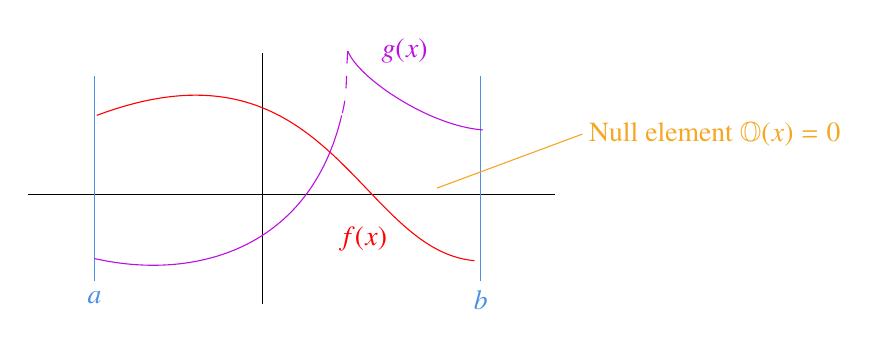
\begin{tikzpicture}[x=0.75pt,y=0.75pt,yscale=-1,xscale=1]
%uncomment if require: \path (0,300); %set diagram left start at 0, and has height of 300

%Straight Lines [id:da28902997561163524] 
\draw    (65,123) -- (319,123) ;
%Straight Lines [id:da33478321711056114] 
\draw    (178,176) -- (178,55) ;
%Curve Lines [id:da28346474586323334] 
\draw [color={rgb, 255:red, 255; green, 0; blue, 0 }  ,draw opacity=1 ]   (98,85) .. controls (210,43) and (224,150) .. (280,155) ;
%Straight Lines [id:da22459181685384633] 
\draw [color={rgb, 255:red, 74; green, 144; blue, 226 }  ,draw opacity=1 ]   (97,165) -- (97,66) ;
%Straight Lines [id:da16540063730298127] 
\draw [color={rgb, 255:red, 74; green, 144; blue, 226 }  ,draw opacity=1 ]   (283,165) -- (283,66) ;
%Curve Lines [id:da9880193058231301] 
\draw [color={rgb, 255:red, 189; green, 16; blue, 224 }  ,draw opacity=1 ]   (97,154) .. controls (146,165) and (201,149) .. (216,85) ;
%Curve Lines [id:da6034716203940473] 
\draw [color={rgb, 255:red, 189; green, 16; blue, 224 }  ,draw opacity=1 ]   (284,92) .. controls (258,90) and (224,67) .. (219,54) ;
%Curve Lines [id:da9212613170532304] 
\draw [color={rgb, 255:red, 189; green, 16; blue, 224 }  ,draw opacity=1 ] [dash pattern={on 4.5pt off 4.5pt}]  (219,54) .. controls (218,63) and (219,75) .. (216,85) ;
%Straight Lines [id:da9949776892336972] 
\draw [color={rgb, 255:red, 245; green, 166; blue, 35 }  ,draw opacity=1 ]   (262,120) -- (332,94) ;

% Text Node
\draw (234,54) node [anchor=west] [inner sep=0.75pt]  [color={rgb, 255:red, 189; green, 16; blue, 224 }  ,opacity=1 ]  {$g( x)$};
% Text Node
\draw (239.16,137.2) node [anchor=north east] [inner sep=0.75pt]  [color={rgb, 255:red, 255; green, 0; blue, 0 }  ,opacity=1 ]  {$f( x)$};
% Text Node
\draw (334,94) node [anchor=west] [inner sep=0.75pt]  [color={rgb, 255:red, 245; green, 166; blue, 35 }  ,opacity=1 ] [align=left] {Null element $\displaystyle \mathbb{O}( x) =0$};
% Text Node
\draw (97,168.4) node [anchor=north] [inner sep=0.75pt]  [color={rgb, 255:red, 74; green, 144; blue, 226 }  ,opacity=1 ]  {$a$};
% Text Node
\draw (283,168.4) node [anchor=north] [inner sep=0.75pt]  [color={rgb, 255:red, 74; green, 144; blue, 226 }  ,opacity=1 ]  {$b$};


\end{tikzpicture}

\end{center}

$
\langle f(x) \mid g(x)\rangle=\displaystyle\int_{a}^{b} f(x) g(x) d x
$

Both of these inner products (for vectors and for functions) are the standard inner product of those vector spaces. Nothing makes them special compared to any other arbitrary inner product, apart from a subjective designation due to their utility.

One might be tempted to define the inner product on \(\mathbb{C}^n\) just as in \(\mathbb{R}^n\) by writing
\[
\langle X \mid Y \rangle = \sum_{k=1}^{n} x_k y_k,
\]
where \(X = (x_1, x_2, \dots, x_n)\) and \(Y = (y_1, y_2, \dots, y_n)\). However, this definition fails for complex vectors because it does not guarantee that \(\langle X \mid X \rangle\) is a real number.

For example, consider the vector \(X\) with \(x_1 = 1+i\). Then,
\[
\langle X \mid X \rangle = \sum_{k=1}^{n} x_k^2,
\]
and in this case,
\[
(1+i)^2 = 1 + 2i + i^2 = 1 + 2i - 1 = 2i,
\]
which is purely imaginary. Since an inner product must yield a real (and nonnegative) value for \(\langle X, X \rangle\) (as only real numbers can be ``positive''), this naive definition is inadequate.

To correct this issue, we modify the definition by conjugating the first entry. The standard definition becomes:
\[
\langle X \mid Y \rangle = \sum_{k=1}^{n} \overline{x_k}\, y_k,
\]
where \(\overline{x_k}\) denotes the complex conjugate of \(x_k\).

This definition ensures that for any vector \(X\),
\[
\langle X \mid X \rangle = \sum_{k=1}^{n} \overline{x_k}\, x_k = \sum_{k=1}^{n} \lvert x_k \rvert^2,
\]
which is always real and nonnegative.

Additionally, the inner product satisfies the conjugate symmetry property, which replaces the first inner product property, $\langle X, Y \rangle = \langle Y, X \rangle$, for complex vector spaces:
\[
\langle X \mid Y \rangle = \overline{\langle Y \mid X \rangle}.
\]
To verify this, note that
\[
\langle Y \mid X \rangle = \sum_{k=1}^{n} \overline{y_k}\, x_k,
\]
and taking the complex conjugate yields
\[
\overline{\langle Y\mid X \rangle} = \overline{\sum_{k=1}^{n} \overline{y_k}\, x_k} = \sum_{k=1}^{n} \overline{x_k}\, y_k = \langle X \mid Y \rangle.
\]

Thus, by defining the inner product as
\[
\langle X \mid Y \rangle = \sum_{k=1}^{n} \overline{x_k}\, y_k,
\]
we ensure that \(\langle X, X \rangle\) is real and nonnegative, and all the axioms of an inner product space are satisfied.

So the 4 axioms are:

$\langle X \mid Y\rangle=\overline{\langle Y \mid X\rangle}$. Conjugate symmetry.

$\langle X \mid Y+Z\rangle=\langle X \mid Y\rangle+\langle X \mid Z\rangle $

$\langle X \mid \alpha Y\rangle=\alpha\langle X \mid Y\rangle$

$\langle X \mid X\rangle \geqslant 0 \text {, and }=0 \text { if and only if } X=0$

Note: $\langle\beta X \mid Y\rangle=\overline{\langle Y \mid \beta X\rangle}=\overline{[\beta\langle Y \mid X\rangle]}=\overline{\beta}\overline{\langle Y \mid X\rangle}=\overline{\beta}\langle X \mid Y\rangle$. So a constant on the left gets complex conjugated.

It should be noted that the modified symmetry axioms $\langle X \mid Y\rangle=\overline{\langle Y \mid X\rangle}$ is just a generalization of the original symmetry axiom. If $X$ and $Y$ are both real, $\langle Y\mid X \rangle = \overline{\langle Y\mid X \rangle}$ anyway.

We could have also defined $\langle X \mid Y\rangle=\sum\limits_{k=1}^{n} x_{k} \overline{y_{k}}$, it is just a matter of convention. In that case, we would have to move homogeneity (axiom 3) to the first element, resulting in $\langle\alpha X \mid  Y\rangle=\alpha\langle X \mid Y\rangle$ and $\langle X \mid \alpha Y\rangle=\overline{\alpha}\langle X \mid Y\rangle$. 

However, we should once again note that if $\alpha$ is a real number, $\overline\alpha = \alpha$, so homogeneity would apply to either element.

This convention is actually a Math vs Physics thing. Most physics texts use the definition presented here, while most mathematics texts use the alternative definition mentioned. That's why if you take MATH 223, you'll likely see the dot product defined as $\langle X \mid Y\rangle=\sum\limits_{k=1}^{n} x_{k} \overline{y_{k}}$.

Eg: Integrable functions on $a \leq x \leq b$.

$$
\begin{aligned}
& f(x)=e^{2 x}(\cos (3 x)+i \sin (3 x)) \\
& g(x)=e^{-x}(\cos (5 x)-i \sin (5 x)) 
\end{aligned}
$$

$\langle f(2) \mid g(2)\rangle=\displaystyle\int_{a}^{b} \overline{f(2)} g(2) d x \text { and } \\$

$\langle f(2) \mid f(2)\rangle=\displaystyle\int_{a}^{b} \overline{f(x)} f(x) d x=\displaystyle\int_{a}^{b}|f(x)|^{2} d x \geqslant 0 \text {, and }=0 \text { only when } f(x)=0$

\chapter{Linear Algebra}

\section{Linear Dependence and Independence}

Let $\bar{V}_1, \bar{V}_2, \bar{V}_3, \ldots, \bar{V}_n$ be nonzero elements in vector space $V$ and $C_1, C_2, C_3, \ldots, C_n \in \mathbb{R}$

If the only solution to $C_1 \bar{V}_1+C_2 \bar{V}_2+C_3 \bar{V}_3+\ldots+ C_n \bar{V}_n=0$ is the trivial solution ( $C_1=C_2=\ldots=C_n=0$ ), the set of $\bar{V}_1, \ldots, \bar{V}_n$ is linearly independent. Otherwise they are linearly dependent.

\section{Wronskian}

If $W\left[f_1, f_2, f_3, \ldots, f_n\right]$ ever $\neq 0$, the set is linearly independent. If $W\left[f_1, f_2, f_3, \ldots, f_n\right]=0$ always and the set af functions are all analytic (can be expressed as a convergent power series on the domain of interest), the set is linearly dependent.

\emph{NB: $f_1, \ldots, f_n$ must be continuous and differentiable on $[a, b]$.}

\section{Dimension and Basis}

Dimension: The dimension of vector space $V$ is the cardinality of the basis of $V$. (number of basis vectors).

Corollary: Any set of vectors with cardinality $>\operatorname{dim}(V)$ is linearly dependent.

Corollary 2: The maximum number of linearly independent vectors is $\operatorname{dim}(V)$.

Basis: A set of linearly independent vectors that span $V$ is a basis of $V$. 

Corollary: All elements in $V$ can be expressed as a linear combination of the elements of a basis of $V$. (Unique to the basis).

i.e. $\begin{array}{l}
     \text{$\{\hat{\imath}, \hat{\jmath}\}$ is a basis in $\mathbb{R}^2$. So is any pair of non colinear vectors. } \\
     \text{$\{\hat{\imath}, \hat{\jmath}, \hat{k}\}$ is a basis in $\mathbb{R}^3$. So are any 3 non coplanar vectors.}
\end{array}$

\section{Linear Operators}

$\tau$ is an operator on $V$ if $\tau \bar{x} \in V$ where $\bar{X} \in V$.

If for any $\bar{x} \in V, c \in \mathbb{R}$.

$$
\tau\left(\bar{x}_1+\bar{x}_2\right)=\tau\left(\bar{x}_1\right)+\tau\left(\bar{x}_2\right) \text { and } \tau(c \bar{x})=c \tau(\bar{x}).
$$

%%%%%%%%%%%%%%%%%%%%

$\tau$ is a linear operator and the image of $\tau: V \rightarrow V$ forms a subspace.

Eg. The operator $\tau=\dfrac{d}{d x}$ is a linear operator on the vector space $V$ of polynomials of degree $n$ or less.

NB: So is the operator $\tau=\displaystyle\int^{x} d t$, but its image is not confined in $V$

$$
\begin{aligned}
& \tau=\dfrac{d}{d x}, \tau: V \rightarrow V \\
& \tau=\displaystyle\int^{x} d x, \tau: V \rightarrow W,\ W=p_{n+1}(x),\ V=p_{n}(x)
\end{aligned}
$$

\section{Null Spaces}

The null space of a linear operator $\mathcal{L}$ on $V$ is the set of elements $v \in V$ s.t. $\mathcal{L} v=\mathbb{O}$.

I.e. The null space of $\mathcal{L}=\dfrac{d}{d x}$ is $v=c,\ c \in \mathbb{R}$.

Obviously, since $\dfrac{d}{d x} c=\mathcal{L} c=0$. The derivative of a constant is zero.

\section{Gram-Schmidt Process}

By definition, $\langle X \mid Y\rangle=|X||Y| \cos (X, Y)$

And, $\langle X \mid X\rangle=|X|^{2},\quad \therefore|X|=\sqrt{\langle X \mid X\rangle}$

The distance between two elements (ie. functions) is:

$$
\operatorname{dist}(f, g)=|f-g|.
$$

The Gram-Schmidt process turns a basis into an orthogonal basis.

Given a basis $\left\{v_{1}, v_{2}, v_{3}, \ldots, v_{n}\right\} \xrightarrow{G-S}\left\{u_{1}, u_{2}, u_{3}, \ldots, u_{n}\right\}$

Orthogonality is defined as $\left\langle u_{n}, u_{k}\right\rangle=0$ if $n \neq k$. The Gram-Schmidt algorithm is as follows:

$$
\begin{aligned}
& u_{1}=v_{1} \\
& u_{2}=v_{2}-\dfrac{\left\langle v_{2}, u_{1}\right\rangle}{\left\langle u_{1}, u_{1}\right\rangle} u_{1} \\
& u_{3}=v_{3}-\dfrac{\left\langle v_{3}, u_{1}\right\rangle}{\left\langle u_{1}, u_{1}\right\rangle} u_{1}-\dfrac{\left\langle v_{3}, u_{2}\right\rangle}{\left\langle u_{2}, u_{2}\right\rangle} u_{2}
\end{aligned}
$$

Essentially it subtracts the non-orthogonal components of the vectors away. Note that the G-S process does not normalize the basis. That has to be done separately.

To normalize, $\varnothing_{1}=\dfrac{u_{1}}{\sqrt{\left\langle u_{1}, u_{1}\right\rangle}}$ for all $u_{n}$.

To get the ``best approximation'' of an element $f$ outside a vector space $V$ (ie. $x^{4}$ in $p_{3}(x)$ ):

$f \approx \sum\limits_{k=1}^{n} a_{k} \phi_{k} \quad$ where $a_{k}=\left\langle\phi_{k}, f\right\rangle$

NOTE: $\varnothing$ must be an orthonormal basis, not just orthogonal.

I.e. Estimate $\tau^{4}$ with $\varnothing=\left\{\frac{1}{\sqrt{2}}, \sqrt{\frac{3}{2}} \tau, \sqrt{\frac{5}{8}}\left(3 \tau^{2}-1\right), \sqrt{\frac{7}{8}}\left(5 \tau^{3}-3 \tau\right)\right\}$

$a_{1}=\left\langle\dfrac{1}{\sqrt{2}}, \tau^{4}\right\rangle$

$a_{2}=\left\langle\sqrt{\dfrac{3}{2}} \tau, \tau^{4}\right\rangle$, and so on for $a_{3}, a_{4}$.

\section{Eigenvalues/Eigenfunctions of Differential Equations.}

For the purposes of this course, consider a general solution like $\Psi(x, t)=\sum\limits_{n=1}^{\infty} A_{n} \sin \left(\dfrac{n \pi x}{L}\right) e^{\frac{-n^{2} \pi^{2}}{L^{2}}\cdot t}$\qquad BVP 1-A

The eigenvalue will be $\dfrac{n^{2} \pi^{2}}{L^{2}}$, the eigenfunction will be $\sin (\sqrt{\lambda} x) e^{-\lambda t}$.

Mathematically, it is in the form:

$$
\mathcal{L}[f(x)]=\lambda f(x)
$$

Where $\mathcal{L}$ is a linear operator (i.e. derivative), $\lambda$ is a scalar eigenvalue, $f(x)$ is the eigenfunction, maintaining shape under $\mathcal{L}$.

I.e. $\mathcal{L}=\dfrac{d^{2}}{d x^{2}}$

$$
\therefore \dfrac{d^{2} f(x)}{d x^{2}}=\lambda f(x)
$$

As always, there are 3 cases $(\lambda>0,\ \lambda=0,\ \lambda<0)$

The only oscillatory solution is $\underbrace{\lambda=-k^{2}}_{\text{eigenvalues}}$

$$\therefore f^{\prime \prime}(x)=-k^{2} f(x)$$

$$
f(x)=A\!\underbrace{\cos(kx)}_{\text{eigenfunction}}+B\!\underbrace{\sin(kx)}_{\text{eigenfunction}}.
$$

The specific values of $\lambda, A, B$ depend on the B.C.s.

I.e. with homogeneous Dirichlet conditions on $x \in[0, L]$ yields

$$
\begin{aligned}
& k=\dfrac{n \pi}{L} \Rightarrow \lambda=-\dfrac{n^{2} \pi^{2}}{L^{2}} \\
& f_{n}(x)=\sin \left(\dfrac{n \pi x}{L}\right).
\end{aligned}
$$

\section{Hermitian Operators}

A Hermitian operator $\mathcal{L}$ over an inner product is a linear operator with the property: $\langle X, \mathcal{L}[Y]\rangle=\langle\mathcal{L}[Y], X\rangle$

The inner product for functions is defined (with real values) by
\[
\langle f, g \rangle = \int_a^b f(x)\, g(x)\, w(x) \, dx,
\]
where \(w(x)\) is a given weight function. 

If \(\mathcal{L}\) is a Hermitian operator, then for all functions \(f(x)\) and \(g(x)\) in the domain of \(\mathcal{L}\), the following equality holds:
\[
\int_a^b f(x)\, \mathcal{L}[g](x) \, dx = \int_a^b \mathcal{L}[f](x)\, g(x) \, dx.
\]

\emph{NB, this is a tough criterion, most operators are not Hermitian.}

Hermitian operators are obviously not absolute. If the inner product is defined differently, a operator may cease to be Hermitian.

Hermitian operators have the following properties:

\begin{enumerate}
  \item \textbf{The eigenvalues of a Hermitian operator are real.} \\
    Let \(\mathcal{L}\) be a Hermitian operator on an inner product space and let \(f\) be an eigenvector of \(\mathcal{L}\) with eigenvalue \(\lambda\), i.e.,
    \[
    \mathcal{L}[f] = \lambda f.
    \]
    Then, using the properties of the inner product, we have
    \[
    \langle f, \mathcal{L}[f] \rangle = \langle f, \lambda f \rangle = \lambda \langle f, f \rangle.
    \]
    Since \(\mathcal{L}\) is Hermitian,
    \[
    \langle f, \mathcal{L}[f] \rangle = \langle \mathcal{L}[f], f \rangle = \langle \lambda f, f \rangle = \overline{\lambda}\langle f, f \rangle.
    \]
    Equating the two expressions and noting that \(\langle f, f \rangle \neq 0\) (since \(f\) is nonzero), we conclude
    \[
    \lambda = \overline{\lambda},
    \]
    which implies that \(\lambda\) is real, as only real numbers are equal to their complex conjugate.

  \item \textbf{The eigenvectors of a Hermitian operator corresponding to different eigenvalues are orthogonal.} \\
    Let \(f\) and \(g\) be eigenvectors of the Hermitian operator \(\mathcal{L}\) corresponding to distinct eigenvalues \(\lambda\) and \(\mu\) respectively:
    \[
    \mathcal{L}[f] = \lambda f \quad \text{and} \quad \mathcal{L}[g] = \mu g.
    \]
    Consider the inner product \(\langle f, \mathcal{L}[g] \rangle\). On one hand, using the eigenvalue equation for \(g\),
    \[
    \langle f, \mathcal{L}[g] \rangle = \langle f, \mu g \rangle = \mu \langle f, g \rangle.
    \]
    On the other hand, using the Hermitian property of \(\mathcal{L}\) and the eigenvalue equation for \(f\),
    \[
    \langle f, \mathcal{L}[g] \rangle = \langle \mathcal{L}[f], g \rangle = \langle \lambda f, g \rangle = \lambda \langle f, g \rangle.
    \]
    Equating these two expressions gives
    \[
    \lambda \langle f, g \rangle = \mu \langle f, g \rangle.
    \]
    Since \(\lambda \neq \mu\), it follows that
    \[
    \langle f, g \rangle = 0,
    \]
    meaning that \(f\) and \(g\) are orthogonal.
\end{enumerate}

An operator being Hermitian may depend on the boundary conditions imposed on the functions. For example, consider the operator
\[
\mathcal{L} = \frac{d^2}{dx^2}.
\]
For \(\mathcal{L}\) to be Hermitian, the boundary term that arises from integration by parts must vanish. To see this, let \(f\) and \(g\) be functions defined on \([0,L]\) and consider
\begin{align*}
\langle \mathcal{L}[f], g \rangle &= \int_0^L \frac{d^2 f}{dx^2}\, g(x)\, dx \\
&= \left[ f'(x) g(x) - f(x) g'(x) \right]_{0}^{L} + \int_0^L f(x) \frac{d^2 g}{dx^2}\, dx \quad \text{(by integration by parts)} \\
&= \text{B.T.} + \langle f, \mathcal{L}[g] \rangle,
\end{align*}
where the boundary term (B.T.) is given by
\[
\text{B.T.} = \left[ f'(x) g(x) - f(x) g'(x) \right]_{0}^{L}.
\]
Thus, for \(\mathcal{L}\) to be Hermitian (i.e., for
\[
\langle \mathcal{L}[f], g \rangle = \langle f, \mathcal{L}[g] \rangle \quad \text{for all } f, g),
\]
the boundary term must vanish:
\[
\left[ f'(x) g(x) - f(x) g'(x) \right]_{0}^{L} = 0.
\]
This condition depends on the specific boundary conditions imposed on the functions.


\section{Parseval's Theorem}

\emph{Optional. There is more to be covered but it gets pretty advanced and not too useful for people without a real analysis or advanced algebra background.}

For $f(x)$ piecewise smooth on $(0, L)$:

$
\begin{aligned}
& f(x)=\sum\limits_{n=1}^{\infty} b_{n} g_{n} \\
& \langle f(x) \mid f(x)\rangle=\left\langle f(x) \mid \sum\limits_{n=1}^{\infty} b_{n} g_{n}\right\rangle=\sum\limits_{n=1}^{\infty} b_{n}\left\langle f(x) \mid g_{n}\right\rangle=\sum\limits_{n=1}^{\infty} b_{n} \cdot \dfrac{L \overline{b_{n}}}{2}=\dfrac{L}{2} \sum\limits_{n=1}^{\infty}\left|b_{n}\right|^{2} \\
& \text{If} \left\langle g_{n} \mid f(x)\right\rangle=\dfrac{L}{2} b_{n} \text {, then }\left\langle f(x) \mid g_{n}\right\rangle=\dfrac{L}{2} \overline{b_{n}}
\end{aligned}
$

$\therefore \dfrac{2}{L}\langle f(x) \mid f(x)\rangle=\sum\limits_{n=1}^{\infty}\left|b_{n}\right|^{2}$

$\therefore \sum\limits_{n=1}^{\infty}\left|b_{n}\right|^{2}=\dfrac{2}{L} \displaystyle\int_{0}^{L}|f(x)|^{2} d x$ \quad Fourier transform is unitary.


\chapter{Sturm–Liouville Boundary Value Problems}

\section{Introduction to Sturm–Liouville Equations}

When solving boundary‐value problems involving the Laplacian \( (\nabla^{2}) \) via separation of variables, one arrives at ordinary differential equations (eigenvalue problems) of the form
\[
\alpha(x)\,y''(x) + \beta(x)\,y'(x) + \gamma(x)\,y(x) \;=\; \lambda\,y(x),
\]
where \(\alpha,\beta,\gamma\) are given coefficient functions.  Such a second‐order linear ODE can always be written in Sturm–Liouville form:
\[
\frac{d}{dx}\bigl(p(x)\,y'(x)\bigr) + q(x)\,y(x) \;=\; \lambda\,w(x)\,y(x).
\]
Indeed, expanding the left‐hand side gives
\[
p(x)\,y''(x) + p'(x)\,y'(x) + q(x)\,y(x) \;=\; \lambda\,w(x)\,y(x),
\]
and, upon dividing by \(p(x)\), one obtains
\[
y''(x) \;+\; \frac{p'(x)}{p(x)}\,y'(x) \;+\; \frac{q(x)}{p(x)}\,y(x) \;=\; \frac{\lambda\,w(x)}{p(x)}\,y(x).
\]
Comparing with
\[
y''(x) \;+\; \frac{\beta(x)}{\alpha(x)}\,y'(x) \;+\; \frac{\gamma(x)}{\alpha(x)}\,y(x) \;=\; \frac{\lambda}{\alpha(x)}\,y(x),
\]
one reads off
\[
\frac{1}{p(x)}\,\frac{dp}{dx}(x) \;=\; \frac{\beta(x)}{\alpha(x)} 
\quad\Longrightarrow\quad
\boxed{p(x) \;=\; \exp\!\Bigl(\int \frac{\beta(x)}{\alpha(x)}\,dx\Bigr)},
\]
\[
\frac{q(x)}{p(x)} \;=\; \frac{\gamma(x)}{\alpha(x)}
\quad\Longrightarrow\quad
\boxed{q(x) \;=\; \frac{\gamma(x)}{\alpha(x)}\,p(x)},
\]
\[
\frac{w(x)}{p(x)} \;=\; \frac{1}{\alpha(x)}
\quad\Longrightarrow\quad
\boxed{w(x) \;=\; \frac{p(x)}{\alpha(x)}}.
\]
Thus the Sturm–Liouville operator
\[
\mathcal{L}\;=\;\frac{d}{dx}\Bigl[p(x)\,\frac{d}{dx}\Bigr] + q(x)
\]
is formally Hermitian provided one imposes appropriate boundary conditions.  In particular, if \(f_{1}\) and \(f_{2}\) are two functions satisfying the same homogeneous boundary conditions, then
\[
\int_{a}^{b} w(x)\,f_{1}(x)\,f_{2}(x)\,dx \;=\; 0
\quad\text{whenever their corresponding eigenvalues are different.}
\]
Equivalently, \(\mathcal{L}\) is self‐adjoint if
\[
\bigl[p(x)\,\bigl(f_{1}'(x)\,f_{2}(x) - f_{1}(x)\,f_{2}'(x)\bigr)\bigr]_{x=a}^{x=b}
\;=\; 0.
\]

There are generally two conditions where this equation holds:

\textbf{A. Homogeneous Boundary Conditions}

This includes homogeneous Dirichlet (\(f(a)=0\)), Neumann (\(f'(a)=0\)), and Robin conditions as special cases.

\begin{itemize}
  \item At \(x = a\): 
    \[
    \text{Either }p(a) = 0,\quad\text{or}\quad C_{1}\,f(a) + C_{2}\,f'(a) = 0.
    \]
  \item At \(x = b\): 
    \[
    \text{Either }p(b) = 0,\quad\text{or}\quad K_{1}\,f(b) + K_{2}\,f'(b) = 0.
    \]
  \item The constants \(C_{1},C_{2}\) (at \(x=a\)) and \(K_{1},K_{2}\) (at \(x=b\)) must be the same for every eigenfunction.
\end{itemize}

\textbf{B. Periodic (Symmetric) Boundary Conditions}

\begin{enumerate}
  \item \(p(a) = p(b)\),
  \item \(f(a) = f(b)\),
  \item \(f'(a) = f'(b)\).
\end{enumerate}

\section{Sturm–Liouville Theorem}

Consider the Sturm–Liouville problem
\[
\frac{d}{dx}\Bigl[p(x)\,\frac{d}{dx}\,y(x)\Bigr] \;+\; q(x)\,y(x) \;=\; \lambda\,w(x)\,y(x),
\]
on the interval \(a \le x \le b\), subject to either homogeneous or periodic boundary conditions.  Assume:
\begin{enumerate}
  \item \(p(x)\in C^{1}[a,b]\) and \(p(x)>0\) on \([a,b]\).
  \item \(q(x)\in C^{0}[a,b]\).
  \item \(w(x)\in C^{0}[a,b]\) and \(w(x)>0\) on \([a,b]\).
  \item The boundary conditions are either homogeneous (Dirichlet, Neumann, or Robin) or periodic as described above.
\end{enumerate}
Then:
\begin{enumerate}
  \item There exists an infinite sequence of real, discrete eigenvalues 
    \(\lambda_{1} < \lambda_{2} < \lambda_{3} < \cdots\), with \(\lambda_{n} \to +\infty\).
  \item The corresponding eigenfunctions \(\{Y_{n}(x)\}\) can be chosen to be real and satisfy
    \[
    \int_{a}^{b} w(x)\,Y_{m}(x)\,Y_{n}(x)\,dx = 0 \quad (m\neq n).
    \]
  \item Any sufficiently smooth function \(f(x)\) defined on \([a,b]\) can be expanded in the orthonormal set \(\{Y_{n}\}\):
    \[
    f(x) \;=\; \sum_{n=1}^{\infty} \beta_{n}\,Y_{n}(x), 
    \qquad
    \beta_{n} 
    \;=\;
    \frac{\displaystyle\int_{a}^{b} w(x)\,f(x)\,Y_{n}(x)\,dx}{\displaystyle\int_{a}^{b} w(x)\,\bigl[Y_{n}(x)\bigr]^{2}\,dx}.
    \]
\end{enumerate}

\section{Examples of Sturm–Liouville BVPs}

Most of the classical boundary‐value problems (for example, homogeneous Dirichlet or Neumann on a finite interval) are special cases of S-L problems.  They can often be solved by ordinary Fourier series, but more general weight functions or boundary conditions require the full S-L machinery.

\subsection{The Simple Dirichlet–Dirichlet Case}

\[
\frac{d^{2}y}{dx^{2}}(x) \;=\; \lambda\,y(x),
\qquad
0 \le x \le L,
\qquad
y(0)=0,\quad y(L)=0,
\]
has eigenvalues and eigenfunctions
\[
\lambda_{n} = -\bigl(\tfrac{n\pi}{L}\bigr)^{2},
\qquad
Y_{n}(x) = \sin\!\Bigl(\tfrac{n\pi x}{L}\Bigr), 
\quad n = 1,2,3,\dots.
\]
One checks that 
\(\int_{0}^{L}\sin(\tfrac{n\pi x}{L})\,\sin(\tfrac{m\pi x}{L})\,dx=0\) whenever \(n\neq m\).

\subsection{A Mixed Boundary‐Value Problem (Robin at \(x=\pi\))}

Consider the heat equation on \(0 < x < \pi,\; t>0\):
\[
\frac{\partial \psi}{\partial t}(x,t) 
\;=\; 
\frac{\partial^{2}\psi}{\partial x^{2}}(x,t),
\]
with boundary conditions 
\[
\psi(0,t)=0,
\qquad
\frac{\partial \psi}{\partial x}(\pi,t)=0
\quad(\text{insulated at }x=\pi),
\]
and initial condition \(\psi(x,0)=f(x)\).  Separation of variables \(\psi(x,t)=X(x)\,T(t)\) leads to
\[
X''(x) \;=\; \lambda\,X(x),
\qquad
X(0)=0,\quad X'(\pi)=0.
\]
Nontrivial solutions exist only when \(\lambda<0\).  Set \(\lambda=-\mu^{2}\) with \(\mu>0\).  Then
\[
X(x) = A\,\sin(\mu\,x) + B\,\cos(\mu\,x),
\quad
X(0)=0 \;\Longrightarrow\; B=0,
\]
\[
X'(x) = A\,\mu\,\cos(\mu\,x),
\qquad
X'(\pi)=0 \;\Longrightarrow\; \cos(\mu\,\pi)=0 
\;\Longrightarrow\; 
\mu\,\pi = \Bigl(2n+1\Bigr)\tfrac{\pi}{2}, 
\quad n=0,1,2,\dots
\]
Hence
\[
\mu_{n} = \frac{2n+1}{2}, 
\qquad
X_{n}(x) = A_{n}\,\sin\!\Bigl(\tfrac{2n+1}{2}\,x\Bigr),
\quad
n=0,1,2,\dots
\]
The corresponding time‐dependent part is 
\[
T_{n}(t) = \exp\Bigl(-\mu_{n}^{2}\,t\Bigr).
\]
Thus
\[
\psi(x,t)
= \sum_{n=0}^{\infty} D_{n}\,\sin\!\Bigl(\tfrac{2n+1}{2}\,x\Bigr)\,
\exp\Bigl(-\bigl(\tfrac{2n+1}{2}\bigr)^{2}t\Bigr).
\]
Enforcing \(\psi(x,0)=f(x)\) gives the expansion
\[
f(x) \;=\; \sum_{n=0}^{\infty} D_{n}\,\sin\!\Bigl(\tfrac{2n+1}{2}\,x\Bigr),
\]
and since
\[
\int_{0}^{\pi} \sin^{2}\!\Bigl(\tfrac{2n+1}{2}\,x\Bigr)\,dx \;=\; \frac{\pi}{2},
\]
one finds
\[
D_{n} \;=\; \frac{\displaystyle\int_{0}^{\pi} f(x)\,\sin\!\bigl(\tfrac{2n+1}{2}\,x\bigr)\,dx}
                {\displaystyle\frac{\pi}{2}}
\;=\; 
\frac{2}{\pi}\,\int_{0}^{\pi} f(x)\,\sin\!\Bigl(\tfrac{2n+1}{2}\,x\Bigr)\,dx.
\]

\section{Legendre Polynomials}

The Legendre differential equation
\[
\frac{d}{dx}\Bigl[(1 - x^{2})\,\frac{dy}{dx}\Bigr] + n(n+1)\,y(x) \;=\; 0,
\qquad -1 \le x \le 1,
\]
is already in Sturm–Liouville form with 
\[
p(x) = 1 - x^{2}, 
\quad
q(x) = 0, 
\quad
w(x) = 1, 
\quad
\lambda = n(n+1).
\]
Its solutions that remain finite on \([-1,1]\) are the Legendre polynomials \(P_{n}(x)\).  One often introduces the change of variable \(x=\cos\varphi\), but the final answer is simply
\[
y(x) = P_{n}(x), 
\qquad x \in [-1,1].
\]
The first few Legendre polynomials are:
\[
\begin{aligned}
P_{0}(x) &= 1,\\
P_{1}(x) &= x,\\
P_{2}(x) &= \frac{1}{2}\,\bigl(3x^{2} - 1\bigr),\\
P_{3}(x) &= \frac{1}{2}\,\bigl(5x^{3} - 3x\bigr).
\end{aligned}
\]
They satisfy the orthogonality relation
\[
\int_{-1}^{1} P_{n}(x)\,P_{m}(x)\,dx = \frac{2}{2n+1}\,\delta_{nm},
\]
so that
\[
P_{n}(x)\;\perp\;P_{m}(x)\quad(n\neq m).
\]
Moreover,
\begin{itemize}
  \item \(P_{n}\) is even if \(n\) is even, and odd if \(n\) is odd.
  \item In particular, \(P_{n}(0) = 0\) whenever \(n\) is odd, and \(P_{n}(0)\neq 0\) when \(n\) is even.
\end{itemize}
Legendre polynomials play a central role in solving spherical boundary‐value problems via series expansions.

\section{BVP 9: Steady-State Temp. in Spherical Regions}

Assume no \(\theta\) dependence, so \(\psi\) depends only on \(r\) and \(\varphi\).  The Laplacian in spherical coordinates is:

\begin{center}
    

% Pattern Info
 
\tikzset{
pattern size/.store in=\mcSize, 
pattern size = 5pt,
pattern thickness/.store in=\mcThickness, 
pattern thickness = 0.3pt,
pattern radius/.store in=\mcRadius, 
pattern radius = 1pt}
\makeatletter
\pgfutil@ifundefined{pgf@pattern@name@_hz4i3zlgq}{
\pgfdeclarepatternformonly[\mcThickness,\mcSize]{_hz4i3zlgq}
{\pgfqpoint{0pt}{0pt}}
{\pgfpoint{\mcSize+\mcThickness}{\mcSize+\mcThickness}}
{\pgfpoint{\mcSize}{\mcSize}}
{
\pgfsetcolor{\tikz@pattern@color}
\pgfsetlinewidth{\mcThickness}
\pgfpathmoveto{\pgfqpoint{0pt}{0pt}}
\pgfpathlineto{\pgfpoint{\mcSize+\mcThickness}{\mcSize+\mcThickness}}
\pgfusepath{stroke}
}}
\makeatother

% Pattern Info
 
\tikzset{
pattern size/.store in=\mcSize, 
pattern size = 5pt,
pattern thickness/.store in=\mcThickness, 
pattern thickness = 0.3pt,
pattern radius/.store in=\mcRadius, 
pattern radius = 1pt}
\makeatletter
\pgfutil@ifundefined{pgf@pattern@name@_w4wodh9hq}{
\pgfdeclarepatternformonly[\mcThickness,\mcSize]{_w4wodh9hq}
{\pgfqpoint{0pt}{0pt}}
{\pgfpoint{\mcSize+\mcThickness}{\mcSize+\mcThickness}}
{\pgfpoint{\mcSize}{\mcSize}}
{
\pgfsetcolor{\tikz@pattern@color}
\pgfsetlinewidth{\mcThickness}
\pgfpathmoveto{\pgfqpoint{0pt}{0pt}}
\pgfpathlineto{\pgfpoint{\mcSize+\mcThickness}{\mcSize+\mcThickness}}
\pgfusepath{stroke}
}}
\makeatother

% Pattern Info
 
\tikzset{
pattern size/.store in=\mcSize, 
pattern size = 5pt,
pattern thickness/.store in=\mcThickness, 
pattern thickness = 0.3pt,
pattern radius/.store in=\mcRadius, 
pattern radius = 1pt}
\makeatletter
\pgfutil@ifundefined{pgf@pattern@name@_sijy7gf30}{
\pgfdeclarepatternformonly[\mcThickness,\mcSize]{_sijy7gf30}
{\pgfqpoint{0pt}{0pt}}
{\pgfpoint{\mcSize+\mcThickness}{\mcSize+\mcThickness}}
{\pgfpoint{\mcSize}{\mcSize}}
{
\pgfsetcolor{\tikz@pattern@color}
\pgfsetlinewidth{\mcThickness}
\pgfpathmoveto{\pgfqpoint{0pt}{0pt}}
\pgfpathlineto{\pgfpoint{\mcSize+\mcThickness}{\mcSize+\mcThickness}}
\pgfusepath{stroke}
}}
\makeatother

% Pattern Info
 
\tikzset{
pattern size/.store in=\mcSize, 
pattern size = 5pt,
pattern thickness/.store in=\mcThickness, 
pattern thickness = 0.3pt,
pattern radius/.store in=\mcRadius, 
pattern radius = 1pt}
\makeatletter
\pgfutil@ifundefined{pgf@pattern@name@_1nww7g8qd}{
\pgfdeclarepatternformonly[\mcThickness,\mcSize]{_1nww7g8qd}
{\pgfqpoint{0pt}{0pt}}
{\pgfpoint{\mcSize+\mcThickness}{\mcSize+\mcThickness}}
{\pgfpoint{\mcSize}{\mcSize}}
{
\pgfsetcolor{\tikz@pattern@color}
\pgfsetlinewidth{\mcThickness}
\pgfpathmoveto{\pgfqpoint{0pt}{0pt}}
\pgfpathlineto{\pgfpoint{\mcSize+\mcThickness}{\mcSize+\mcThickness}}
\pgfusepath{stroke}
}}
\makeatother
\tikzset{every picture/.style={line width=0.75pt}} %set default line width to 0.75pt        

\begin{tikzpicture}[x=0.75pt,y=0.75pt,yscale=-1,xscale=1]
%uncomment if require: \path (0,511); %set diagram left start at 0, and has height of 511

%Shape: Path Data [id:dp5545507714497666] 
\draw  [color={rgb, 255:red, 65; green, 117; blue, 5 }  ,draw opacity=1 ][pattern=_hz4i3zlgq,pattern size=6pt,pattern thickness=0.75pt,pattern radius=0pt, pattern color={rgb, 255:red, 65; green, 117; blue, 5}] (454,200.98) .. controls (419.51,200.98) and (390.04,184.97) .. (378.26,162.38) .. controls (378.09,160.27) and (378,158.15) .. (378,156) .. controls (378,147.82) and (379.29,139.94) .. (381.68,132.56) .. controls (395.14,144.23) and (422.47,152.22) .. (454,152.22) .. controls (485.53,152.22) and (512.86,144.23) .. (526.32,132.56) .. controls (528.71,139.94) and (530,147.82) .. (530,156) .. controls (530,158.15) and (529.91,160.27) .. (529.74,162.38) .. controls (517.96,184.97) and (488.49,200.98) .. (454,200.98) -- cycle ;
%Shape: Path Data [id:dp504781126009527] 
\draw  [color={rgb, 255:red, 245; green, 166; blue, 35 }  ,draw opacity=1 ][pattern=_w4wodh9hq,pattern size=6pt,pattern thickness=0.75pt,pattern radius=0pt, pattern color={rgb, 255:red, 255; green, 155; blue, 0}] (454,80) .. controls (487.79,80) and (516.44,102.06) .. (526.32,132.56) .. controls (512.86,144.23) and (485.53,152.22) .. (454,152.22) .. controls (422.47,152.22) and (395.14,144.23) .. (381.68,132.56) .. controls (391.56,102.06) and (420.21,80) .. (454,80) -- cycle (400.16,102.36) .. controls (410.42,109.3) and (430.68,114.02) .. (454,114.02) .. controls (477.32,114.02) and (497.58,109.3) .. (507.84,102.36) .. controls (494.08,88.55) and (475.04,80) .. (454,80) .. controls (432.96,80) and (413.92,88.55) .. (400.16,102.36) -- cycle ;
%Shape: Path Data [id:dp21177902583713037] 
\draw  [draw opacity=0] (454,200.98) .. controls (419.51,200.98) and (390.04,184.97) .. (378.26,162.38) .. controls (378.09,160.27) and (378,158.15) .. (378,156) .. controls (378,114.03) and (412.03,80) .. (454,80) .. controls (495.97,80) and (530,114.03) .. (530,156) .. controls (530,158.15) and (529.91,160.27) .. (529.74,162.38) .. controls (517.96,184.97) and (488.49,200.98) .. (454,200.98) -- cycle ;
%Shape: Path Data [id:dp24631649628407404] 
\draw  [color={rgb, 255:red, 255; green, 0; blue, 0 }  ,draw opacity=1 ][pattern=_sijy7gf30,pattern size=6pt,pattern thickness=0.75pt,pattern radius=0pt, pattern color={rgb, 255:red, 255; green, 0; blue, 0}] (454,80) .. controls (475.04,80) and (494.08,88.55) .. (507.84,102.36) .. controls (497.58,109.3) and (477.32,114.02) .. (454,114.02) .. controls (430.68,114.02) and (410.42,109.3) .. (400.16,102.36) .. controls (413.92,88.55) and (432.96,80) .. (454,80) -- cycle ;
%Shape: Path Data [id:dp8502022999443875] 
\draw  [draw opacity=0] (454,80) .. controls (487.79,80) and (516.44,102.06) .. (526.32,132.56) .. controls (512.86,144.23) and (485.53,152.22) .. (454,152.22) .. controls (422.47,152.22) and (395.14,144.23) .. (381.68,132.56) .. controls (391.56,102.06) and (420.21,80) .. (454,80) -- cycle ;
%Shape: Path Data [id:dp4900369177835193] 
\draw  [draw opacity=0][pattern=_1nww7g8qd,pattern size=6pt,pattern thickness=0.75pt,pattern radius=0pt, pattern color={rgb, 255:red, 74; green, 144; blue, 226}] (454,232) .. controls (414.17,232) and (381.5,201.37) .. (378.26,162.38) .. controls (390.04,184.97) and (419.51,200.98) .. (454,200.98) .. controls (488.49,200.98) and (517.96,184.97) .. (529.74,162.38) .. controls (526.5,201.37) and (493.83,232) .. (454,232) -- cycle ;
%Shape: Circle [id:dp6219218788853764] 
\draw  [line width=1.5]  (84,156) .. controls (84,114.03) and (118.03,80) .. (160,80) .. controls (201.97,80) and (236,114.03) .. (236,156) .. controls (236,197.97) and (201.97,232) .. (160,232) .. controls (118.03,232) and (84,197.97) .. (84,156) -- cycle ;
%Shape: Arc [id:dp07478306771265375] 
\draw  [draw opacity=0] (236.72,155.33) .. controls (233.37,169.15) and (200.53,180) .. (160.5,180) .. controls (118.25,180) and (84,167.91) .. (84,153) -- (160.5,153) -- cycle ; \draw   (236.72,155.33) .. controls (233.37,169.15) and (200.53,180) .. (160.5,180) .. controls (118.25,180) and (84,167.91) .. (84,153) ;  
%Shape: Arc [id:dp6162285887763814] 
\draw  [draw opacity=0][dash pattern={on 4.5pt off 4.5pt}] (236.72,155.33) .. controls (233.51,140.84) and (200.6,129.45) .. (160.48,129.45) .. controls (118.23,129.45) and (83.98,142.08) .. (83.98,157.66) -- (160.48,157.66) -- cycle ; \draw  [dash pattern={on 4.5pt off 4.5pt}] (236.72,155.33) .. controls (233.51,140.84) and (200.6,129.45) .. (160.48,129.45) .. controls (118.23,129.45) and (83.98,142.08) .. (83.98,157.66) ;  
%Shape: Arc [id:dp8214720919175589] 
\draw  [draw opacity=0][dash pattern={on 4.5pt off 4.5pt}] (158.1,80.02) .. controls (157.9,80.01) and (157.69,80) .. (157.49,80) .. controls (142.03,80) and (129.49,113.8) .. (129.49,155.5) .. controls (129.49,196.71) and (141.74,230.21) .. (156.95,230.99) -- (157.49,155.5) -- cycle ; \draw  [dash pattern={on 4.5pt off 4.5pt}] (158.1,80.02) .. controls (157.9,80.01) and (157.69,80) .. (157.49,80) .. controls (142.03,80) and (129.49,113.8) .. (129.49,155.5) .. controls (129.49,196.71) and (141.74,230.21) .. (156.95,230.99) ;  
%Shape: Arc [id:dp3521260124073198] 
\draw  [draw opacity=0] (161.89,80.78) .. controls (176.66,86.06) and (188,117.5) .. (188,155.5) .. controls (188,196.75) and (174.63,230.28) .. (158.03,230.99) -- (157.49,155.5) -- cycle ; \draw   (161.89,80.78) .. controls (176.66,86.06) and (188,117.5) .. (188,155.5) .. controls (188,196.75) and (174.63,230.28) .. (158.03,230.99) ;  
%Straight Lines [id:da7800760641044076] 
\draw    (160.48,157.66) -- (280,157.66) ;
%Straight Lines [id:da8726440979847523] 
\draw    (160.48,157.66) -- (160.48,46) ;
%Straight Lines [id:da2223974616382236] 
\draw    (160.48,157.66) -- (77,215) ;
%Straight Lines [id:da4746498605386775] 
\draw [color={rgb, 255:red, 255; green, 0; blue, 0 }  ,draw opacity=1 ]   (160.48,157.66) -- (186,131) ;
%Straight Lines [id:da3526632912210763] 
\draw [color={rgb, 255:red, 255; green, 0; blue, 0 }  ,draw opacity=1 ]   (160.48,157.66) -- (187,179) ;
%Straight Lines [id:da7669986372649702] 
\draw [color={rgb, 255:red, 253; green, 0; blue, 0 }  ,draw opacity=1 ] [dash pattern={on 4.5pt off 4.5pt}]  (186,131) -- (187,179) ;
%Curve Lines [id:da8794193860154438] 
\draw [color={rgb, 255:red, 255; green, 0; blue, 0 }  ,draw opacity=1 ]   (161,141) .. controls (165,139) and (173,141) .. (173.24,144.33) ;
%Curve Lines [id:da9319109674142974] 
\draw [color={rgb, 255:red, 255; green, 0; blue, 0 }  ,draw opacity=1 ]   (151,164) .. controls (155,169) and (163,168) .. (169,166) ;
%Shape: Arc [id:dp3225353685799819] 
\draw  [draw opacity=0] (529.72,155.33) .. controls (526.37,169.15) and (493.53,180) .. (453.5,180) .. controls (411.25,180) and (377,167.91) .. (377,153) -- (453.5,153) -- cycle ; \draw   (529.72,155.33) .. controls (526.37,169.15) and (493.53,180) .. (453.5,180) .. controls (411.25,180) and (377,167.91) .. (377,153) ;  
%Shape: Arc [id:dp6464563944466906] 
\draw  [draw opacity=0][dash pattern={on 4.5pt off 4.5pt}] (529.72,155.33) .. controls (526.51,140.84) and (493.6,129.45) .. (453.48,129.45) .. controls (411.23,129.45) and (376.98,142.08) .. (376.98,157.66) -- (453.48,157.66) -- cycle ; \draw  [dash pattern={on 4.5pt off 4.5pt}] (529.72,155.33) .. controls (526.51,140.84) and (493.6,129.45) .. (453.48,129.45) .. controls (411.23,129.45) and (376.98,142.08) .. (376.98,157.66) ;  
%Shape: Arc [id:dp9679597616846731] 
\draw  [draw opacity=0][dash pattern={on 4.5pt off 4.5pt}] (451.1,80.02) .. controls (450.9,80.01) and (450.69,80) .. (450.49,80) .. controls (435.03,80) and (422.49,113.8) .. (422.49,155.5) .. controls (422.49,196.71) and (434.74,230.21) .. (449.95,230.99) -- (450.49,155.5) -- cycle ; \draw  [dash pattern={on 4.5pt off 4.5pt}] (451.1,80.02) .. controls (450.9,80.01) and (450.69,80) .. (450.49,80) .. controls (435.03,80) and (422.49,113.8) .. (422.49,155.5) .. controls (422.49,196.71) and (434.74,230.21) .. (449.95,230.99) ;  
%Shape: Arc [id:dp040014308201230975] 
\draw  [draw opacity=0] (454.89,80.78) .. controls (469.66,86.06) and (481,117.5) .. (481,155.5) .. controls (481,196.75) and (467.63,230.28) .. (451.03,230.99) -- (450.49,155.5) -- cycle ; \draw   (454.89,80.78) .. controls (469.66,86.06) and (481,117.5) .. (481,155.5) .. controls (481,196.75) and (467.63,230.28) .. (451.03,230.99) ;  
%Straight Lines [id:da2942605869147963] 
\draw    (453.48,157.66) -- (573,157.66) ;
%Straight Lines [id:da14801733407989337] 
\draw    (453.48,157.66) -- (453.48,46) ;
%Straight Lines [id:da5999225336789571] 
\draw    (453.48,157.66) -- (370,215) ;
%Shape: Circle [id:dp7493871364294102] 
\draw  [line width=1.5]  (377,156) .. controls (377,114.03) and (411.03,80) .. (453,80) .. controls (494.97,80) and (529,114.03) .. (529,156) .. controls (529,197.97) and (494.97,232) .. (453,232) .. controls (411.03,232) and (377,197.97) .. (377,156) -- cycle ;
%Shape: Circle [id:dp18648732179421224] 
\draw  [draw opacity=0][fill={rgb, 255:red, 255; green, 0; blue, 0 }  ,fill opacity=1 ] (183.7,131) .. controls (183.7,129.73) and (184.73,128.7) .. (186,128.7) .. controls (187.27,128.7) and (188.3,129.73) .. (188.3,131) .. controls (188.3,132.27) and (187.27,133.3) .. (186,133.3) .. controls (184.73,133.3) and (183.7,132.27) .. (183.7,131) -- cycle ;
%Shape: Circle [id:dp6904776384442068] 
\draw  [draw opacity=0][fill={rgb, 255:red, 255; green, 0; blue, 0 }  ,fill opacity=1 ] (451.18,157.96) .. controls (451.18,156.69) and (452.21,155.66) .. (453.48,155.66) .. controls (454.75,155.66) and (455.78,156.69) .. (455.78,157.96) .. controls (455.78,159.23) and (454.75,160.26) .. (453.48,160.26) .. controls (452.21,160.26) and (451.18,159.23) .. (451.18,157.96) -- cycle ;

% Text Node
\draw (372,218.4) node [anchor=north west][inner sep=0.75pt]    {$x$};
% Text Node
\draw (575,157.66) node [anchor=west] [inner sep=0.75pt]    {$y$};
% Text Node
\draw (455.48,42.6) node [anchor=south west] [inner sep=0.75pt]    {$z$};
% Text Node
\draw (176.24,135.93) node [anchor=south east] [inner sep=0.75pt]  [font=\footnotesize,color={rgb, 255:red, 255; green, 0; blue, 0 }  ,opacity=1 ]  {$\varphi $};
% Text Node
\draw (167,169.4) node [anchor=north east] [inner sep=0.75pt]  [font=\footnotesize,color={rgb, 255:red, 255; green, 0; blue, 0 }  ,opacity=1 ]  {$\theta $};
% Text Node
\draw (184.5,150) node [anchor=east] [inner sep=0.75pt]  [font=\footnotesize,color={rgb, 255:red, 255; green, 0; blue, 0 }  ,opacity=1 ]  {$r$};
% Text Node
\draw (79,218.4) node [anchor=north west][inner sep=0.75pt]    {$x$};
% Text Node
\draw (282,157.66) node [anchor=west] [inner sep=0.75pt]    {$y$};
% Text Node
\draw (162.48,42.6) node [anchor=south west] [inner sep=0.75pt]    {$z$};
% Text Node
\draw (276,88.4) node [anchor=north west][inner sep=0.75pt]    {$\xrightarrow{\theta -\text{indep.}}$};


\end{tikzpicture}

\end{center}
\[
\nabla^{2}\psi(r,\varphi)
=
\frac{1}{r^{2}}\frac{\partial}{\partial r}\!\Bigl[r^{2}\,\frac{\partial \psi}{\partial r}\Bigr]
\;+\;
\frac{1}{r^{2}\sin(\varphi)}\,\frac{\partial}{\partial \varphi}\!\Bigl[\sin(\varphi)\,\frac{\partial \psi}{\partial \varphi}\Bigr]
\;=\;0.
\]
Apply separation of variables, \(\psi(r,\varphi) = R(r)\,L(\varphi)\).  Substitute into \(\nabla^{2}\psi=0\) and divide by \(R\,L\):
\[
\frac{1}{R}\,\frac{d}{dr}\!\Bigl[r^{2}\,\frac{dR}{dr}\Bigr]
\;+\;
\frac{1}{L\,\sin(\varphi)}\,\frac{d}{d\varphi}\!\Bigl[\sin(\varphi)\,\frac{dL}{d\varphi}\Bigr]
\;=\;0.
\]
Since the first term depends only on \(r\) and the second only on \(\varphi\), each must equal a constant \(\lambda\).  Thus
\[
\frac{1}{R}\,\frac{d}{dr}\!\Bigl[r^{2}\,\frac{dR}{dr}\Bigr]
\;=\;
-\,\frac{1}{L\,\sin(\varphi)}\,\frac{d}{d\varphi}\!\Bigl[\sin(\varphi)\,\frac{dL}{d\varphi}\Bigr]
\;=\;\lambda.
\]

First, consider the radial part:
\[
\frac{d}{dr}\!\Bigl[r^{2}\,\frac{dR}{dr}\Bigr] \;=\; \lambda\,R(r).
\]
This is an Euler–Cauchy equation.  Assume \(R(r) = r^{k}\).  Then
\[
\frac{dR}{dr} = k\,r^{k-1}, 
\quad
\frac{d^{2}R}{dr^{2}} = (k-1)\,k\,r^{\,k-2},
\]
so
\[
r^{2}\,(k-1)\,k\,r^{\,k-2} \;+\; 2r\,\bigl(k\,r^{\,k-1}\bigr) \;-\; \lambda\,r^{\,k} \;=\; 0
\;\;\Longrightarrow\;\;
(k^{2} + k - \lambda)\,r^{\,k} = 0,
\]
\[
k^{2} + k - \lambda = 0 
\;\;\Longrightarrow\;\;
k_{1,2} = \frac{-1 \pm \sqrt{1 + 4\lambda}}{2}.
\]
Set \(\sqrt{1 + 4\lambda} = 2n + 1\), so \(\lambda = n(n+1)\).  Then
\[
k_{1} = n,\quad
k_{2} = -\,n - 1.
\]
Hence the general radial solution is
\[
\boxed{%
R_{n}(r) \;=\; A_{n}\,r^{n} \;+\; B_{n}\,r^{-\,n-1},%
}
\]
with \(P(r)=r^{2}\), \(q(r)=0\), \(w(r)=1\) in Sturm–Liouville form.

Next, the angular part:
\[
-\,\frac{1}{L(\varphi)\,\sin(\varphi)}\,
\frac{d}{d\varphi}\!\Bigl[\sin(\varphi)\,\frac{dL}{d\varphi}\Bigr]
\;=\;\lambda \;=\; n(n+1).
\]
Let \(x = \cos(\varphi)\).  Then 
\(\frac{d}{d\varphi} = -\,\sin(\varphi)\,\frac{d}{dx}\) and one checks
\[
\frac{1}{\sin(\varphi)}\,\frac{d}{d\varphi}\!\Bigl[\sin(\varphi)\,\frac{dL}{d\varphi}\Bigr]
\;=\;
\frac{d}{dx}\!\Bigl[(1 - x^{2})\,\frac{dL}{dx}\Bigr].
\]
Thus the angular ODE becomes
\[
\frac{d}{dx}\!\Bigl[(1 - x^{2})\,\frac{dL}{dx}\Bigr] + n(n+1)\,L(x) \;=\; 0,
\qquad -1 \le x \le 1,
\]
which is the Legendre equation.  The bounded solutions are the Legendre polynomials \(P_{n}(x)\).  In Sturm–Liouville form, \(P(x)=1 - x^{2}\), \(q(x)=0\), \(w(x)=1\), \(\lambda=n(n+1)\).  Therefore
\[
\boxed{%
L_{n}(x) \;=\; C_{n}\,P_{n}(x), 
\quad x = \cos(\varphi),\;n=0,1,2,\dots.
}
\]
Combining radial and angular parts:
\[
\boxed{%
\psi_{n}(r,\varphi)
= \bigl[A_{n}\,r^{n} + B_{n}\,r^{-\,n-1}\bigr]\,P_{n}(\cos\varphi).
}
\]
Hence the general steady‐state solution is
\[
\boxed{%
\psi(r,\varphi)
= 
\sum_{n=0}^{\infty}
\bigl[A_{n}\,r^{n} + B_{n}\,r^{-\,n-1}\bigr]\;P_{n}(\cos\varphi).
}
\]

\subsection{BVP 9a: Interior Sphere}

\begin{center}
    

\tikzset{every picture/.style={line width=0.75pt}} %set default line width to 0.75pt        

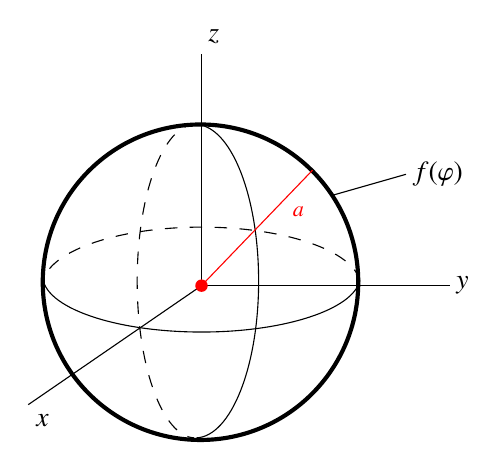
\begin{tikzpicture}[x=0.75pt,y=0.75pt,yscale=-1,xscale=1]
%uncomment if require: \path (0,511); %set diagram left start at 0, and has height of 511

%Shape: Circle [id:dp14934440830523532] 
\draw  [line width=1.5]  (84,156) .. controls (84,114.03) and (118.03,80) .. (160,80) .. controls (201.97,80) and (236,114.03) .. (236,156) .. controls (236,197.97) and (201.97,232) .. (160,232) .. controls (118.03,232) and (84,197.97) .. (84,156) -- cycle ;
%Shape: Arc [id:dp1214166957817917] 
\draw  [draw opacity=0] (236.72,155.33) .. controls (233.37,169.15) and (200.53,180) .. (160.5,180) .. controls (118.25,180) and (84,167.91) .. (84,153) -- (160.5,153) -- cycle ; \draw   (236.72,155.33) .. controls (233.37,169.15) and (200.53,180) .. (160.5,180) .. controls (118.25,180) and (84,167.91) .. (84,153) ;  
%Shape: Arc [id:dp4491292591346454] 
\draw  [draw opacity=0][dash pattern={on 4.5pt off 4.5pt}] (236.72,155.33) .. controls (233.51,140.84) and (200.6,129.45) .. (160.48,129.45) .. controls (118.23,129.45) and (83.98,142.08) .. (83.98,157.66) -- (160.48,157.66) -- cycle ; \draw  [dash pattern={on 4.5pt off 4.5pt}] (236.72,155.33) .. controls (233.51,140.84) and (200.6,129.45) .. (160.48,129.45) .. controls (118.23,129.45) and (83.98,142.08) .. (83.98,157.66) ;  
%Shape: Arc [id:dp2566153017664021] 
\draw  [draw opacity=0][dash pattern={on 4.5pt off 4.5pt}] (158.1,80.02) .. controls (157.9,80.01) and (157.69,80) .. (157.49,80) .. controls (142.03,80) and (129.49,113.8) .. (129.49,155.5) .. controls (129.49,196.71) and (141.74,230.21) .. (156.95,230.99) -- (157.49,155.5) -- cycle ; \draw  [dash pattern={on 4.5pt off 4.5pt}] (158.1,80.02) .. controls (157.9,80.01) and (157.69,80) .. (157.49,80) .. controls (142.03,80) and (129.49,113.8) .. (129.49,155.5) .. controls (129.49,196.71) and (141.74,230.21) .. (156.95,230.99) ;  
%Shape: Arc [id:dp8623515290830754] 
\draw  [draw opacity=0] (161.89,80.78) .. controls (176.66,86.06) and (188,117.5) .. (188,155.5) .. controls (188,196.75) and (174.63,230.28) .. (158.03,230.99) -- (157.49,155.5) -- cycle ; \draw   (161.89,80.78) .. controls (176.66,86.06) and (188,117.5) .. (188,155.5) .. controls (188,196.75) and (174.63,230.28) .. (158.03,230.99) ;  
%Straight Lines [id:da4169751367520922] 
\draw    (160.48,157.66) -- (280,157.66) ;
%Straight Lines [id:da615019222278173] 
\draw    (160.48,157.66) -- (160.48,46) ;
%Straight Lines [id:da31267781917423454] 
\draw    (160.48,157.66) -- (77,215) ;
%Straight Lines [id:da295919957911442] 
\draw [color={rgb, 255:red, 255; green, 0; blue, 0 }  ,draw opacity=1 ]   (160.48,157.66) -- (214,102) ;
%Straight Lines [id:da13659470423053333] 
\draw    (224,114) -- (259,104) ;
%Shape: Circle [id:dp7403482786634643] 
\draw  [draw opacity=0][fill={rgb, 255:red, 255; green, 0; blue, 0 }  ,fill opacity=1 ] (157.48,157.66) .. controls (157.48,156) and (158.82,154.66) .. (160.48,154.66) .. controls (162.13,154.66) and (163.48,156) .. (163.48,157.66) .. controls (163.48,159.31) and (162.13,160.66) .. (160.48,160.66) .. controls (158.82,160.66) and (157.48,159.31) .. (157.48,157.66) -- cycle ;

% Text Node
\draw (203.24,118.23) node [anchor=north west][inner sep=0.75pt]  [font=\footnotesize,color={rgb, 255:red, 255; green, 0; blue, 0 }  ,opacity=1 ]  {$a$};
% Text Node
\draw (79,218.4) node [anchor=north west][inner sep=0.75pt]    {$x$};
% Text Node
\draw (282,157.66) node [anchor=west] [inner sep=0.75pt]    {$y$};
% Text Node
\draw (162.48,42.6) node [anchor=south west] [inner sep=0.75pt]    {$z$};
% Text Node
\draw (261,104) node [anchor=west] [inner sep=0.75pt]    {$f( \varphi )$};


\end{tikzpicture}

\end{center}

\[
\begin{cases}
\nabla^{2}\psi = 0, 
\quad 0 \le r \le a,\\
\psi\bigl(a,\varphi\bigr) = f(\varphi) = F\bigl(\cos\varphi\bigr).
\end{cases}
\]
To remain finite at \(r=0\), set \(B_{n}=0\).  Then
\[
\psi(r,\varphi) 
= 
\sum_{n=0}^{\infty} A_{n}\,r^{n}\,P_{n}(\cos\varphi).
\]
Impose \(\psi(a,\varphi) = F(x)\) with \(x=\cos\varphi\):
\[
\sum_{n=0}^{\infty} A_{n}\,a^{n}\,P_{n}(x) 
= F(x).
\]
By orthogonality,
\(\int_{-1}^{1}P_{n}(x)\,P_{m}(x)\,dx = \tfrac{2}{2n+1}\,\delta_{nm},\)
so
\[
A_{n}\,a^{n} 
= 
\beta_{n} 
= 
\frac{\displaystyle\int_{-1}^{1}F(x)\,P_{n}(x)\,dx}
     {\displaystyle\int_{-1}^{1}\bigl[P_{n}(x)\bigr]^{2}\,dx}
= 
\frac{2n+1}{2}\,
\int_{-1}^{1}F(x)\,P_{n}(x)\,dx.
\]
Therefore
\[
\boxed{%
A_{n} 
= 
\frac{2n+1}{2\,a^{n}}\,
\int_{-1}^{1}F(x)\,P_{n}(x)\,dx,
\quad
\psi(r,\varphi)
= \sum_{n=0}^{\infty}
\Bigl[\tfrac{2n+1}{2\,a^{n}}
\!\!\int_{-1}^{1}F(x)\,P_{n}(x)\,dx\Bigr]\,r^{n}\,P_{n}(\cos\varphi).
}
\]

\subsection{BVP 9b: Exterior Sphere}

\[
\begin{cases}
\nabla^{2}\psi = 0, 
\quad r \ge a,\\
\psi\bigl(a,\varphi\bigr) = f(\varphi) = F\bigl(\cos\varphi\bigr).
\end{cases}
\]
To remain bounded as \(r \to \infty\), set \(A_{n}=0\).  Then
\[
\psi(r,\varphi) 
= 
\sum_{n=0}^{\infty} B_{n}\,r^{-\,n-1}\,P_{n}(\cos\varphi).
\]
At \(r=a\),
\[
\sum_{n=0}^{\infty} B_{n}\,a^{-\,n-1}\,P_{n}(x) 
= F(x).
\]
Orthogonality gives
\[
B_{n}\,a^{-\,n-1} 
= 
\frac{\displaystyle\int_{-1}^{1}F(x)\,P_{n}(x)\,dx}
     {\displaystyle\int_{-1}^{1}\bigl[P_{n}(x)\bigr]^{2}\,dx}
= 
\frac{2n+1}{2}\,
\int_{-1}^{1}F(x)\,P_{n}(x)\,dx.
\]
Hence
\[
\boxed{%
B_{n} 
= 
\frac{2n+1}{2}\,a^{\,n+1}\,
\int_{-1}^{1}F(x)\,P_{n}(x)\,dx,
\quad
\psi(r,\varphi)
= \sum_{n=0}^{\infty}
\Bigl[\tfrac{2n+1}{2}\,a^{\,n+1}\!
\int_{-1}^{1}F(x)\,P_{n}(x)\,dx\Bigr]\,r^{-\,n-1}\,P_{n}(\cos\varphi).
}
\]

\subsection{BVP 9c: Steady-State Temperature Between Two Cocentric Spheres}

Let the inner surface \(r=a\) be held at \(f(\varphi) = F(x)\), and the outer \(r=b\) at \(g(\varphi) = G(x)\).  Then
\[
\begin{cases}
\nabla^{2}\psi = 0, 
\quad a \le r \le b,\\
\psi\bigl(a,\varphi\bigr) = F(x),\qquad
\psi\bigl(b,\varphi\bigr) = G(x),
\end{cases}
\]
and the general solution is
\[
\psi(r,\varphi)
= \sum_{n=0}^{\infty}
\bigl[A_{n}\,r^{n} + B_{n}\,r^{-\,n-1}\bigr]\;P_{n}(x),
\quad x=\cos\varphi.
\]
Applying the boundary conditions:
\[
\begin{cases}
A_{n}\,a^{n} + B_{n}\,a^{-\,n-1}
= 
\alpha_{n}
= 
\frac{2n+1}{2}\,
\int_{-1}^{1}F(x)\,P_{n}(x)\,dx, 
\\
A_{n}\,b^{n} + B_{n}\,b^{-\,n-1}
= 
\gamma_{n}
= 
\frac{2n+1}{2}\,
\int_{-1}^{1}G(x)\,P_{n}(x)\,dx.
\end{cases}
\]
Solve for \(A_{n},B_{n}\) (a \(2\times2\) system):
\[
\boxed{%
A_{n} 
= 
\frac{\alpha_{n}\,b^{\,n+1} \;-\; \gamma_{n}\,a^{\,n+1}}
     {\,b^{\,n+1}\,a^{\,n} \;-\; a^{\,n+1}\,b^{\,n}\,},
\quad
B_{n} 
= 
\frac{\gamma_{n}\,a^{\,n}\,b^{\,n+1} \;-\; \alpha_{n}\,a^{\,n+1}\,b^{\,n}}
     {\,b^{\,n+1}\,a^{\,n} \;-\; a^{\,n+1}\,b^{\,n}\,}.
}
\]
Therefore the solution between the two spheres is
\[
\boxed{%
\psi(r,\varphi)
= 
\sum_{n=0}^{\infty}
\Biggl[
\frac{\alpha_{n}\,b^{\,n+1} - \gamma_{n}\,a^{\,n+1}}
     {\,b^{\,n+1}\,a^{\,n} - a^{\,n+1}\,b^{\,n}\,}\;r^{n}
\;+\;
\frac{\gamma_{n}\,a^{\,n}\,b^{\,n+1} - \alpha_{n}\,a^{\,n+1}\,b^{\,n}}
     {\,b^{\,n+1}\,a^{\,n} - a^{\,n+1}\,b^{\,n}\,}\;r^{-\,n-1}
\Biggr]\,P_{n}(\cos\varphi).
}
\]

I know this looks a bit scary. Just do a few problems, and it'll be easier than it seems. 

\section{BVP 10: Steady-State Temp. in Cylindrical Regions}

Assume no \(\theta\) dependence, so \(\psi = \psi(r,z)\).  There are three boundaries: at \(z=0\), \(z=H\), and \(r=b\), which must be treated separately.  The general solution is obtained by superposition:
\[
\psi(r,z) \;=\; \psi_{\text{side}}(r,z)
\;+\;\psi_{\text{top}}(r,z)
\;+\;\psi_{\text{bottom}}(r,z).
\]

\begin{center}
    

% Pattern Info
 
\tikzset{
pattern size/.store in=\mcSize, 
pattern size = 5pt,
pattern thickness/.store in=\mcThickness, 
pattern thickness = 0.3pt,
pattern radius/.store in=\mcRadius, 
pattern radius = 1pt}
\makeatletter
\pgfutil@ifundefined{pgf@pattern@name@_j9ysr5onf}{
\pgfdeclarepatternformonly[\mcThickness,\mcSize]{_j9ysr5onf}
{\pgfqpoint{0pt}{0pt}}
{\pgfpoint{\mcSize+\mcThickness}{\mcSize+\mcThickness}}
{\pgfpoint{\mcSize}{\mcSize}}
{
\pgfsetcolor{\tikz@pattern@color}
\pgfsetlinewidth{\mcThickness}
\pgfpathmoveto{\pgfqpoint{0pt}{0pt}}
\pgfpathlineto{\pgfpoint{\mcSize+\mcThickness}{\mcSize+\mcThickness}}
\pgfusepath{stroke}
}}
\makeatother

% Pattern Info
 
\tikzset{
pattern size/.store in=\mcSize, 
pattern size = 5pt,
pattern thickness/.store in=\mcThickness, 
pattern thickness = 0.3pt,
pattern radius/.store in=\mcRadius, 
pattern radius = 1pt}
\makeatletter
\pgfutil@ifundefined{pgf@pattern@name@_q043580j2}{
\pgfdeclarepatternformonly[\mcThickness,\mcSize]{_q043580j2}
{\pgfqpoint{0pt}{0pt}}
{\pgfpoint{\mcSize+\mcThickness}{\mcSize+\mcThickness}}
{\pgfpoint{\mcSize}{\mcSize}}
{
\pgfsetcolor{\tikz@pattern@color}
\pgfsetlinewidth{\mcThickness}
\pgfpathmoveto{\pgfqpoint{0pt}{0pt}}
\pgfpathlineto{\pgfpoint{\mcSize+\mcThickness}{\mcSize+\mcThickness}}
\pgfusepath{stroke}
}}
\makeatother
\tikzset{every picture/.style={line width=0.75pt}} %set default line width to 0.75pt        

\begin{tikzpicture}[x=0.75pt,y=0.75pt,yscale=-1,xscale=1]
%uncomment if require: \path (0,300); %set diagram left start at 0, and has height of 300

%Shape: Ellipse [id:dp96915205168507] 
\draw  [pattern=_j9ysr5onf,pattern size=6pt,pattern thickness=0.75pt,pattern radius=0pt, pattern color={rgb, 255:red, 208; green, 2; blue, 27}][dash pattern={on 4.5pt off 4.5pt}] (46,214.5) .. controls (46,205.39) and (59.43,198) .. (76,198) .. controls (92.57,198) and (106,205.39) .. (106,214.5) .. controls (106,223.61) and (92.57,231) .. (76,231) .. controls (59.43,231) and (46,223.61) .. (46,214.5) -- cycle ;
%Shape: Can [id:dp17106850982348099] 
\draw   (106,111.5) -- (106,214.5) .. controls (106,223.61) and (92.57,231) .. (76,231) .. controls (59.43,231) and (46,223.61) .. (46,214.5) -- (46,111.5) .. controls (46,102.39) and (59.43,95) .. (76,95) .. controls (92.57,95) and (106,102.39) .. (106,111.5) .. controls (106,120.61) and (92.57,128) .. (76,128) .. controls (59.43,128) and (46,120.61) .. (46,111.5) ;
%Shape: Ellipse [id:dp15605417005031086] 
\draw  [pattern=_q043580j2,pattern size=6pt,pattern thickness=0.75pt,pattern radius=0pt, pattern color={rgb, 255:red, 74; green, 144; blue, 226}] (46,111.5) .. controls (46,102.39) and (59.43,95) .. (76,95) .. controls (92.57,95) and (106,102.39) .. (106,111.5) .. controls (106,120.61) and (92.57,128) .. (76,128) .. controls (59.43,128) and (46,120.61) .. (46,111.5) -- cycle ;
%Straight Lines [id:da6277486957754892] 
\draw    (76,214.5) -- (176,214.5) ;
%Straight Lines [id:da5195387959422559] 
\draw    (76,214.5) -- (76,72) ;
%Straight Lines [id:da11296344129799718] 
\draw    (76,214.5) -- (22.5,268) ;
%Straight Lines [id:da33439541400508976] 
\draw    (128,211.5) -- (128,117) ;
\draw [shift={(128,117)}, rotate = 90] [color={rgb, 255:red, 0; green, 0; blue, 0 }  ][line width=0.75]    (0,5.59) -- (0,-5.59)   ;
\draw [shift={(128,211.5)}, rotate = 90] [color={rgb, 255:red, 0; green, 0; blue, 0 }  ][line width=0.75]    (0,5.59) -- (0,-5.59)   ;
%Straight Lines [id:da511601202121384] 
\draw [color={rgb, 255:red, 65; green, 117; blue, 5 }  ,draw opacity=1 ]   (46,111.5) -- (46,214.5) ;
%Straight Lines [id:da7559333328373139] 
\draw [color={rgb, 255:red, 65; green, 117; blue, 5 }  ,draw opacity=1 ]   (106,111.5) -- (106,214.5) ;
%Straight Lines [id:da1608253780960347] 
\draw [color={rgb, 255:red, 65; green, 117; blue, 5 }  ,draw opacity=1 ]   (78,161.5) -- (104,161.5) ;
\draw [shift={(104,161.5)}, rotate = 180] [color={rgb, 255:red, 65; green, 117; blue, 5 }  ,draw opacity=1 ][line width=0.75]    (0,5.59) -- (0,-5.59)   ;
\draw [shift={(78,161.5)}, rotate = 180] [color={rgb, 255:red, 65; green, 117; blue, 5 }  ,draw opacity=1 ][line width=0.75]    (0,5.59) -- (0,-5.59)   ;
%Straight Lines [id:da6733452684906849] 
\draw [color={rgb, 255:red, 255; green, 0; blue, 0 }  ,draw opacity=1 ]   (86,225) -- (117,245) ;
%Straight Lines [id:da7798938773834545] 
\draw [color={rgb, 255:red, 74; green, 144; blue, 226 }  ,draw opacity=1 ]   (89,113) -- (117,81) ;

% Text Node
\draw (213.5,215.4) node [anchor=north] [inner sep=0.75pt]    {$\pi $};
% Text Node
\draw (130,164.25) node [anchor=west] [inner sep=0.75pt]    {$H$};
% Text Node
\draw (44,163) node [anchor=east] [inner sep=0.75pt]  [color={rgb, 255:red, 65; green, 117; blue, 5 }  ,opacity=1 ]  {$g( z)$};
% Text Node
\draw (92,164.9) node [anchor=north] [inner sep=0.75pt]  [color={rgb, 255:red, 65; green, 117; blue, 5 }  ,opacity=1 ]  {$b$};
% Text Node
\draw (119,248.4) node [anchor=north west][inner sep=0.75pt]  [color={rgb, 255:red, 252; green, 0; blue, 0 }  ,opacity=1 ]  {$h( r)$};
% Text Node
\draw (119,77.6) node [anchor=south west] [inner sep=0.75pt]  [color={rgb, 255:red, 74; green, 144; blue, 226 }  ,opacity=1 ]  {$f( r)$};


\end{tikzpicture}

\end{center}

We impose
\[
\nabla^{2}\psi = 0,\quad
\psi(r,0) = h(r),\quad
\psi(r,H) = f(r),\quad
\psi(b,z) = g(z),
\quad
0 \le r \le b,\;0 \le z \le H.
\]

Laplace’s equation in cylindrical coordinates (no \(\theta\)) is
\[
\frac{1}{r}\,\frac{\partial}{\partial r}\!\Bigl[r\,\frac{\partial \psi}{\partial r}\Bigr]
\;+\;
\frac{\partial^{2}\psi}{\partial z^{2}}
\;=\;0.
\]

\vspace{0.5em}
\noindent\textbf{(a) Side‐Boundary Problem:}  
Set \(\psi_{\text{side}}(r,z) = R(r)\,S(z)\) and enforce
\[
\begin{cases}
\nabla^{2}\psi_{\text{side}} = 0,\\
\psi_{\text{side}}(r,0) = 0,\\
\psi_{\text{side}}(r,H) = 0,\\
\psi_{\text{side}}(b,z) = g(z).
\end{cases}
\]


\begin{center}
    

% Pattern Info
 
\tikzset{
pattern size/.store in=\mcSize, 
pattern size = 5pt,
pattern thickness/.store in=\mcThickness, 
pattern thickness = 0.3pt,
pattern radius/.store in=\mcRadius, 
pattern radius = 1pt}
\makeatletter
\pgfutil@ifundefined{pgf@pattern@name@_j9ysr5onf}{
\pgfdeclarepatternformonly[\mcThickness,\mcSize]{_j9ysr5onf}
{\pgfqpoint{0pt}{0pt}}
{\pgfpoint{\mcSize+\mcThickness}{\mcSize+\mcThickness}}
{\pgfpoint{\mcSize}{\mcSize}}
{
\pgfsetcolor{\tikz@pattern@color}
\pgfsetlinewidth{\mcThickness}
\pgfpathmoveto{\pgfqpoint{0pt}{0pt}}
\pgfpathlineto{\pgfpoint{\mcSize+\mcThickness}{\mcSize+\mcThickness}}
\pgfusepath{stroke}
}}
\makeatother

% Pattern Info
 
\tikzset{
pattern size/.store in=\mcSize, 
pattern size = 5pt,
pattern thickness/.store in=\mcThickness, 
pattern thickness = 0.3pt,
pattern radius/.store in=\mcRadius, 
pattern radius = 1pt}
\makeatletter
\pgfutil@ifundefined{pgf@pattern@name@_q043580j2}{
\pgfdeclarepatternformonly[\mcThickness,\mcSize]{_q043580j2}
{\pgfqpoint{0pt}{0pt}}
{\pgfpoint{\mcSize+\mcThickness}{\mcSize+\mcThickness}}
{\pgfpoint{\mcSize}{\mcSize}}
{
\pgfsetcolor{\tikz@pattern@color}
\pgfsetlinewidth{\mcThickness}
\pgfpathmoveto{\pgfqpoint{0pt}{0pt}}
\pgfpathlineto{\pgfpoint{\mcSize+\mcThickness}{\mcSize+\mcThickness}}
\pgfusepath{stroke}
}}
\makeatother
\tikzset{every picture/.style={line width=0.75pt}} %set default line width to 0.75pt        

\begin{tikzpicture}[x=0.75pt,y=0.75pt,yscale=-1,xscale=1]
%uncomment if require: \path (0,300); %set diagram left start at 0, and has height of 300

%Shape: Ellipse [id:dp96915205168507] 
\draw  [pattern=_j9ysr5onf,pattern size=6pt,pattern thickness=0.75pt,pattern radius=0pt, pattern color={rgb, 255:red, 208; green, 2; blue, 27}][dash pattern={on 4.5pt off 4.5pt}] (46,214.5) .. controls (46,205.39) and (59.43,198) .. (76,198) .. controls (92.57,198) and (106,205.39) .. (106,214.5) .. controls (106,223.61) and (92.57,231) .. (76,231) .. controls (59.43,231) and (46,223.61) .. (46,214.5) -- cycle ;
%Shape: Can [id:dp17106850982348099] 
\draw   (106,111.5) -- (106,214.5) .. controls (106,223.61) and (92.57,231) .. (76,231) .. controls (59.43,231) and (46,223.61) .. (46,214.5) -- (46,111.5) .. controls (46,102.39) and (59.43,95) .. (76,95) .. controls (92.57,95) and (106,102.39) .. (106,111.5) .. controls (106,120.61) and (92.57,128) .. (76,128) .. controls (59.43,128) and (46,120.61) .. (46,111.5) ;
%Shape: Ellipse [id:dp15605417005031086] 
\draw  [pattern=_q043580j2,pattern size=6pt,pattern thickness=0.75pt,pattern radius=0pt, pattern color={rgb, 255:red, 74; green, 144; blue, 226}] (46,111.5) .. controls (46,102.39) and (59.43,95) .. (76,95) .. controls (92.57,95) and (106,102.39) .. (106,111.5) .. controls (106,120.61) and (92.57,128) .. (76,128) .. controls (59.43,128) and (46,120.61) .. (46,111.5) -- cycle ;
%Straight Lines [id:da6277486957754892] 
\draw    (76,214.5) -- (176,214.5) ;
%Straight Lines [id:da5195387959422559] 
\draw    (76,214.5) -- (76,72) ;
%Straight Lines [id:da11296344129799718] 
\draw    (76,214.5) -- (22.5,268) ;
%Straight Lines [id:da33439541400508976] 
\draw    (128,211.5) -- (128,117) ;
\draw [shift={(128,117)}, rotate = 90] [color={rgb, 255:red, 0; green, 0; blue, 0 }  ][line width=0.75]    (0,5.59) -- (0,-5.59)   ;
\draw [shift={(128,211.5)}, rotate = 90] [color={rgb, 255:red, 0; green, 0; blue, 0 }  ][line width=0.75]    (0,5.59) -- (0,-5.59)   ;
%Straight Lines [id:da511601202121384] 
\draw [color={rgb, 255:red, 65; green, 117; blue, 5 }  ,draw opacity=1 ]   (46,111.5) -- (46,214.5) ;
%Straight Lines [id:da7559333328373139] 
\draw [color={rgb, 255:red, 65; green, 117; blue, 5 }  ,draw opacity=1 ]   (106,111.5) -- (106,214.5) ;
%Straight Lines [id:da1608253780960347] 
\draw [color={rgb, 255:red, 65; green, 117; blue, 5 }  ,draw opacity=1 ]   (78,161.5) -- (104,161.5) ;
\draw [shift={(104,161.5)}, rotate = 180] [color={rgb, 255:red, 65; green, 117; blue, 5 }  ,draw opacity=1 ][line width=0.75]    (0,5.59) -- (0,-5.59)   ;
\draw [shift={(78,161.5)}, rotate = 180] [color={rgb, 255:red, 65; green, 117; blue, 5 }  ,draw opacity=1 ][line width=0.75]    (0,5.59) -- (0,-5.59)   ;
%Straight Lines [id:da6733452684906849] 
\draw [color={rgb, 255:red, 255; green, 0; blue, 0 }  ,draw opacity=1 ]   (86,225) -- (117,245) ;
%Straight Lines [id:da7798938773834545] 
\draw [color={rgb, 255:red, 74; green, 144; blue, 226 }  ,draw opacity=1 ]   (89,113) -- (117,81) ;

% Text Node
\draw (213.5,215.4) node [anchor=north] [inner sep=0.75pt]    {$\pi $};
% Text Node
\draw (130,164.25) node [anchor=west] [inner sep=0.75pt]    {$H$};
% Text Node
\draw (44,163) node [anchor=east] [inner sep=0.75pt]  [color={rgb, 255:red, 65; green, 117; blue, 5 }  ,opacity=1 ]  {$g( z)$};
% Text Node
\draw (92,164.9) node [anchor=north] [inner sep=0.75pt]  [color={rgb, 255:red, 65; green, 117; blue, 5 }  ,opacity=1 ]  {$b$};
% Text Node
\draw (119,248.4) node [anchor=north west][inner sep=0.75pt]  [color={rgb, 255:red, 252; green, 0; blue, 0 }  ,opacity=1 ]  {$0$};
% Text Node
\draw (119,77.6) node [anchor=south west] [inner sep=0.75pt]  [color={rgb, 255:red, 74; green, 144; blue, 226 }  ,opacity=1 ]  {$0$};


\end{tikzpicture}

\end{center}

Substitute \(\psi_{\text{side}} = R(r)\,S(z)\) into Laplace’s equation, divide by \(R\,S\):
\[
\frac{1}{r\,R}\,\frac{d}{dr}\!\Bigl[r\,R'\Bigr]
\;+\;
\frac{1}{S}\,S'' \;=\; 0
\quad\Longrightarrow\quad
\frac{1}{r\,R}\,\frac{d}{dr}\!\bigl[r\,R'(r)\bigr]
= -\,\frac{1}{S(z)}\,S''(z) = \lambda.
\]
Thus
\[
S'' + \lambda\,S = 0,\quad S(0)=0,\;S(H)=0 
\;\Longrightarrow\;
\lambda_{n} = \Bigl(\tfrac{n\pi}{H}\Bigr)^{2},\quad
S_{n}(z) = \sin\!\Bigl(\tfrac{n\pi\,z}{H}\Bigr).
\]
The radial equation is
\[
r\,\frac{d}{dr}\!\Bigl[r\,R'\Bigr]
- \Bigl(\tfrac{n\pi}{H}\Bigr)^{2}\,r^{2}R = 0,
\]
i.e.\ the modified Bessel equation of order zero.  Let \(x = \frac{n\pi\,r}{H}\).  Then
\[
R_{n}(r) = A_{n}\,I_{0}\bigl(x\bigr) + B_{n}\,K_{0}\bigl(x\bigr).
\]
Boundedness at \(r=0\) forces \(B_{n}=0\), so
\[
\boxed{%
R_{n}(r) = I_{0}\!\Bigl(\tfrac{n\pi\,r}{H}\Bigr).
}
\]
Hence
\[
\psi_{\text{side}}(r,z)
= \sum_{n=1}^{\infty}
D_{n}\,I_{0}\!\Bigl(\tfrac{n\pi\,r}{H}\Bigr)\,\sin\!\Bigl(\tfrac{n\pi\,z}{H}\Bigr).
\]
Enforce \(\psi_{\text{side}}(b,z)=g(z)\):
\[
\sum_{n=1}^{\infty}
D_{n}\,I_{0}\!\Bigl(\tfrac{n\pi\,b}{H}\Bigr)\,\sin\!\Bigl(\tfrac{n\pi\,z}{H}\Bigr)
= g(z).
\]
By orthogonality on \([0,H]\),
\[
D_{n}\,I_{0}\!\Bigl(\tfrac{n\pi\,b}{H}\Bigr)
= \frac{2}{H}
\int_{0}^{H} g(z)\,\sin\!\Bigl(\tfrac{n\pi\,z}{H}\Bigr)\,dz,
\]
so
\[
\boxed{%
D_{n}
= 
\frac{2}{\,H\,I_{0}(\tfrac{n\pi\,b}{H})\,}
\int_{0}^{H} g(z)\,\sin\!\Bigl(\tfrac{n\pi\,z}{H}\Bigr)\,dz,
\quad
\psi_{\text{side}}(r,z)
= \sum_{n=1}^{\infty}
\Bigl[\tfrac{2}{H\,I_{0}(\tfrac{n\pi b}{H})}\!
\int_{0}^{H} g(z)\,\sin(\tfrac{n\pi\,z}{H})\,dz\Bigr]\,
I_{0}\!\bigl(\tfrac{n\pi\,r}{H}\bigr)\,\sin\!\bigl(\tfrac{n\pi\,z}{H}\bigr).
}
\]

\begin{center}


\tikzset{every picture/.style={line width=0.75pt}} %set default line width to 0.75pt        

\begin{tikzpicture}[x=0.75pt,y=0.75pt,yscale=-1,xscale=1]
%uncomment if require: \path (0,300); %set diagram left start at 0, and has height of 300

%Straight Lines [id:da1184386906436119] 
\draw    (79,191) -- (360,191) ;
%Straight Lines [id:da5165494151018528] 
\draw    (111,220) -- (111,24) ;
%Curve Lines [id:da841370372902849] 
\draw    (124,50) .. controls (154,116) and (211,158) .. (313,166) ;
%Curve Lines [id:da6663705241092022] 
\draw    (111,160) .. controls (213,160) and (260,135) .. (301,49) ;

% Text Node
\draw (109,160) node [anchor=east] [inner sep=0.75pt]    {$1$};
% Text Node
\draw (303,49) node [anchor=west] [inner sep=0.75pt]    {$I_{0}( x)$};
% Text Node
\draw (315,166) node [anchor=west] [inner sep=0.75pt]    {$K_{0}( x)$};
% Text Node
\draw (39,128) node [anchor=west] [inner sep=0.75pt]  [color={rgb, 255:red, 74; green, 144; blue, 226 }  ,opacity=1 ]  {$I_{0}( 0) =1$};


\end{tikzpicture}

\end{center}

\vspace{0.5em}
\noindent\textbf{(b) Top‐Boundary Problem:}  
Set \(\psi_{\text{top}}(r,z) = R(r)\,S(z)\) and enforce
\[
\begin{cases}
\nabla^{2}\psi_{\text{top}} = 0,\\
\psi_{\text{top}}(r,0) = 0,\\
\psi_{\text{top}}(r,H) = f(r),\\
\psi_{\text{top}}(b,z) = 0.
\end{cases}
\]

\begin{center}
    

% Pattern Info
 
\tikzset{
pattern size/.store in=\mcSize, 
pattern size = 5pt,
pattern thickness/.store in=\mcThickness, 
pattern thickness = 0.3pt,
pattern radius/.store in=\mcRadius, 
pattern radius = 1pt}
\makeatletter
\pgfutil@ifundefined{pgf@pattern@name@_m18gq9d1r}{
\pgfdeclarepatternformonly[\mcThickness,\mcSize]{_m18gq9d1r}
{\pgfqpoint{0pt}{0pt}}
{\pgfpoint{\mcSize+\mcThickness}{\mcSize+\mcThickness}}
{\pgfpoint{\mcSize}{\mcSize}}
{
\pgfsetcolor{\tikz@pattern@color}
\pgfsetlinewidth{\mcThickness}
\pgfpathmoveto{\pgfqpoint{0pt}{0pt}}
\pgfpathlineto{\pgfpoint{\mcSize+\mcThickness}{\mcSize+\mcThickness}}
\pgfusepath{stroke}
}}
\makeatother

% Pattern Info
 
\tikzset{
pattern size/.store in=\mcSize, 
pattern size = 5pt,
pattern thickness/.store in=\mcThickness, 
pattern thickness = 0.3pt,
pattern radius/.store in=\mcRadius, 
pattern radius = 1pt}
\makeatletter
\pgfutil@ifundefined{pgf@pattern@name@_y3t371wzl}{
\pgfdeclarepatternformonly[\mcThickness,\mcSize]{_y3t371wzl}
{\pgfqpoint{0pt}{0pt}}
{\pgfpoint{\mcSize+\mcThickness}{\mcSize+\mcThickness}}
{\pgfpoint{\mcSize}{\mcSize}}
{
\pgfsetcolor{\tikz@pattern@color}
\pgfsetlinewidth{\mcThickness}
\pgfpathmoveto{\pgfqpoint{0pt}{0pt}}
\pgfpathlineto{\pgfpoint{\mcSize+\mcThickness}{\mcSize+\mcThickness}}
\pgfusepath{stroke}
}}
\makeatother
\tikzset{every picture/.style={line width=0.75pt}} %set default line width to 0.75pt        

\begin{tikzpicture}[x=0.75pt,y=0.75pt,yscale=-1,xscale=1]
%uncomment if require: \path (0,300); %set diagram left start at 0, and has height of 300

%Shape: Ellipse [id:dp96915205168507] 
\draw  [pattern=_m18gq9d1r,pattern size=6pt,pattern thickness=0.75pt,pattern radius=0pt, pattern color={rgb, 255:red, 208; green, 2; blue, 27}][dash pattern={on 4.5pt off 4.5pt}] (46,214.5) .. controls (46,205.39) and (59.43,198) .. (76,198) .. controls (92.57,198) and (106,205.39) .. (106,214.5) .. controls (106,223.61) and (92.57,231) .. (76,231) .. controls (59.43,231) and (46,223.61) .. (46,214.5) -- cycle ;
%Shape: Can [id:dp17106850982348099] 
\draw   (106,111.5) -- (106,214.5) .. controls (106,223.61) and (92.57,231) .. (76,231) .. controls (59.43,231) and (46,223.61) .. (46,214.5) -- (46,111.5) .. controls (46,102.39) and (59.43,95) .. (76,95) .. controls (92.57,95) and (106,102.39) .. (106,111.5) .. controls (106,120.61) and (92.57,128) .. (76,128) .. controls (59.43,128) and (46,120.61) .. (46,111.5) ;
%Shape: Ellipse [id:dp15605417005031086] 
\draw  [pattern=_y3t371wzl,pattern size=6pt,pattern thickness=0.75pt,pattern radius=0pt, pattern color={rgb, 255:red, 74; green, 144; blue, 226}] (46,111.5) .. controls (46,102.39) and (59.43,95) .. (76,95) .. controls (92.57,95) and (106,102.39) .. (106,111.5) .. controls (106,120.61) and (92.57,128) .. (76,128) .. controls (59.43,128) and (46,120.61) .. (46,111.5) -- cycle ;
%Straight Lines [id:da6277486957754892] 
\draw    (76,214.5) -- (176,214.5) ;
%Straight Lines [id:da5195387959422559] 
\draw    (76,214.5) -- (76,72) ;
%Straight Lines [id:da11296344129799718] 
\draw    (76,214.5) -- (22.5,268) ;
%Straight Lines [id:da33439541400508976] 
\draw    (128,211.5) -- (128,117) ;
\draw [shift={(128,117)}, rotate = 90] [color={rgb, 255:red, 0; green, 0; blue, 0 }  ][line width=0.75]    (0,5.59) -- (0,-5.59)   ;
\draw [shift={(128,211.5)}, rotate = 90] [color={rgb, 255:red, 0; green, 0; blue, 0 }  ][line width=0.75]    (0,5.59) -- (0,-5.59)   ;
%Straight Lines [id:da511601202121384] 
\draw [color={rgb, 255:red, 65; green, 117; blue, 5 }  ,draw opacity=1 ]   (46,111.5) -- (46,214.5) ;
%Straight Lines [id:da7559333328373139] 
\draw [color={rgb, 255:red, 65; green, 117; blue, 5 }  ,draw opacity=1 ]   (106,111.5) -- (106,214.5) ;
%Straight Lines [id:da1608253780960347] 
\draw [color={rgb, 255:red, 65; green, 117; blue, 5 }  ,draw opacity=1 ]   (78,161.5) -- (104,161.5) ;
\draw [shift={(104,161.5)}, rotate = 180] [color={rgb, 255:red, 65; green, 117; blue, 5 }  ,draw opacity=1 ][line width=0.75]    (0,5.59) -- (0,-5.59)   ;
\draw [shift={(78,161.5)}, rotate = 180] [color={rgb, 255:red, 65; green, 117; blue, 5 }  ,draw opacity=1 ][line width=0.75]    (0,5.59) -- (0,-5.59)   ;
%Straight Lines [id:da6733452684906849] 
\draw [color={rgb, 255:red, 255; green, 0; blue, 0 }  ,draw opacity=1 ]   (86,225) -- (117,245) ;
%Straight Lines [id:da7798938773834545] 
\draw [color={rgb, 255:red, 74; green, 144; blue, 226 }  ,draw opacity=1 ]   (89,113) -- (117,81) ;

% Text Node
\draw (213.5,215.4) node [anchor=north] [inner sep=0.75pt]    {$\pi $};
% Text Node
\draw (130,164.25) node [anchor=west] [inner sep=0.75pt]    {$H$};
% Text Node
\draw (44,163) node [anchor=east] [inner sep=0.75pt]  [color={rgb, 255:red, 65; green, 117; blue, 5 }  ,opacity=1 ]  {$0$};
% Text Node
\draw (92,164.9) node [anchor=north] [inner sep=0.75pt]  [color={rgb, 255:red, 65; green, 117; blue, 5 }  ,opacity=1 ]  {$b$};
% Text Node
\draw (119,248.4) node [anchor=north west][inner sep=0.75pt]  [color={rgb, 255:red, 252; green, 0; blue, 0 }  ,opacity=1 ]  {$0$};
% Text Node
\draw (119,77.6) node [anchor=south west] [inner sep=0.75pt]  [color={rgb, 255:red, 74; green, 144; blue, 226 }  ,opacity=1 ]  {$f( r)$};


\end{tikzpicture}

\end{center}

Separation gives
\[
\frac{1}{r\,R}\,\frac{d}{dr}\!\Bigl[r\,\frac{dR}{dr}\Bigr]
\;+\;
\frac{1}{S}\,\frac{d^{2}S}{dz^{2}}
= 0
\;\Longrightarrow\;
\frac{1}{r\,R}\,\frac{d}{dr}\!\bigl[r\,R'\bigr] = \lambda,\;
\frac{1}{S}\,S'' = -\,\lambda.
\]
The \(z\)–ODE is 
\[
S'' + \lambda\,S = 0,\quad S(0)=0,\;S(H)\text{ free}.
\]
The \(r\)–ODE will enforce \(R(b)=0\).  We choose \(\lambda_{k} = \bigl(\tfrac{\beta_{k}}{b}\bigr)^{2}\), where \(\beta_{k}\) is the \(k\)th zero of \(J_{0}(x)\).  Then
\[
R_{k}(r) = J_{0}\!\bigl(\mu_{k}\,r\bigr), \quad \mu_{k} = \tfrac{\beta_{k}}{b}.
\]
Since \(J_{0}(\beta_{k})=0\), \(R_{k}(b)=0\).  The \(z\)–ODE becomes
\[
S_{k}'' - \mu_{k}^{2}\,S_{k} = 0,\quad S_{k}(0)=0,
\]
whose solution is
\[
S_{k}(z) = A_{k}\,\sinh(\mu_{k}\,z).
\]
Hence
\[
\psi_{\text{top}}(r,z)
= \sum_{k=1}^{\infty}
E_{k}\,J_{0}(\mu_{k}\,r)\,\sinh(\mu_{k}\,z).
\]
Impose \(\psi_{\text{top}}(r,H) = f(r)\):
\[
\sum_{k=1}^{\infty}
E_{k}\,J_{0}(\mu_{k}\,r)\,\sinh(\mu_{k}\,H)
\;=\; f(r),\quad 0 \le r \le b.
\]
By orthogonality with weight \(r\):
\[
E_{k}\,\sinh(\mu_{k}\,H)\int_{0}^{b} r\,\bigl[J_{0}(\mu_{k}r)\bigr]^{2}dr
= \int_{0}^{b} r\,f(r)\,J_{0}(\mu_{k}r)\,dr.
\]
Using 
\(\displaystyle \int_{0}^{b} r\,[J_{0}(\mu_{k}r)]^{2}dr 
= \frac{b^{2}}{2}\,J_{1}(\beta_{k})^{2},\)
we get
\[
E_{k}\,\sinh(\mu_{k}\,H)\frac{b^{2}}{2}J_{1}(\beta_{k})^{2}
= \int_{0}^{b} r\,f(r)\,J_{0}(\mu_{k}r)\,dr,
\]
so
\[
\boxed{%
E_{k}
=
\frac{2}
     {\,b^{2}\,J_{1}(\beta_{k})^{2}\,\sinh(\mu_{k}\,H)\,}\,
\int_{0}^{b} r\,f(r)\,J_{0}(\mu_{k}r)\,dr,
\quad
\psi_{\text{top}}(r,z)
= \sum_{k=1}^{\infty}
\Bigl[\tfrac{2}{b^{2}J_{1}(\beta_{k})^{2}\sinh(\mu_{k}H)}
\!\int_{0}^{b} r\,f(r)\,J_{0}(\mu_{k}r)\,dr\Bigr]\,
J_{0}(\mu_{k}r)\,\sinh(\mu_{k}\,z).
}
\]

\begin{center}
    

\tikzset{every picture/.style={line width=0.75pt}} %set default line width to 0.75pt        

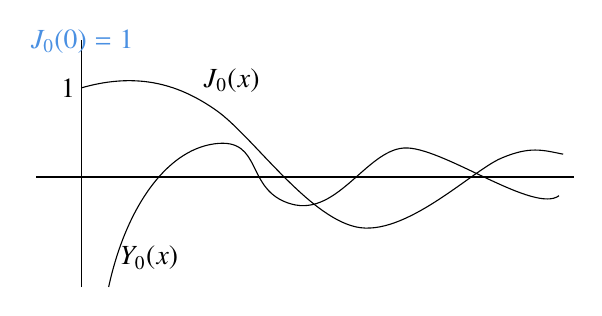
\begin{tikzpicture}[x=0.75pt,y=0.75pt,yscale=-1,xscale=1]
%uncomment if require: \path (0,511); %set diagram left start at 0, and has height of 511

%Straight Lines [id:da9668971146193441] 
\draw    (111,224) -- (370,224) ;
%Straight Lines [id:da5942331351756713] 
\draw    (133,277) -- (133,158) ;
%Curve Lines [id:da6542075612267035] 
\draw    (133,181) .. controls (161,173) and (181,180) .. (198,192) .. controls (215,204) and (241.46,242.56) .. (265,248) .. controls (288.54,253.44) and (321,221) .. (335,215) .. controls (349,209) and (355,211) .. (365,213) ;
%Curve Lines [id:da35929137470118766] 
\draw    (146,277) .. controls (154,240) and (173.13,211.21) .. (197,208) .. controls (220.87,204.79) and (211.27,230.57) .. (234,237) .. controls (256.73,243.43) and (271.09,209.15) .. (290,210) .. controls (308.91,210.85) and (351.3,241.78) .. (363,233) ;

% Text Node
\draw (131,181) node [anchor=east] [inner sep=0.75pt]    {$1$};
% Text Node
\draw (190,184.6) node [anchor=south west] [inner sep=0.75pt]    {$J_{0}(x)$};
\draw (150,270) node [anchor=south west] [inner sep=0.75pt]    {$Y_{0}(x)$};
% Text Node
\draw (133,165.6) node [anchor=south] [inner sep=0.75pt]  [color={rgb, 255:red, 74; green, 144; blue, 226 }  ,opacity=1 ]  {$J_{0}( 0) =1$};


\end{tikzpicture}

\end{center}

\vspace{0.5em}
\noindent\textbf{(c) Bottom‐Boundary Problem:}  
Set \(\psi_{\text{bottom}}(r,z) = R(r)\,S(z)\) and enforce
\[
\begin{cases}
\nabla^{2}\psi_{\text{bottom}} = 0,\\
\psi_{\text{bottom}}(r,0) = h(r),\\
\psi_{\text{bottom}}(r,H) = 0,\\
\psi_{\text{bottom}}(b,z) = 0.
\end{cases}
\]

\begin{center}
    

% Pattern Info
 
\tikzset{
pattern size/.store in=\mcSize, 
pattern size = 5pt,
pattern thickness/.store in=\mcThickness, 
pattern thickness = 0.3pt,
pattern radius/.store in=\mcRadius, 
pattern radius = 1pt}
\makeatletter
\pgfutil@ifundefined{pgf@pattern@name@_8q6btet6w}{
\pgfdeclarepatternformonly[\mcThickness,\mcSize]{_8q6btet6w}
{\pgfqpoint{0pt}{0pt}}
{\pgfpoint{\mcSize+\mcThickness}{\mcSize+\mcThickness}}
{\pgfpoint{\mcSize}{\mcSize}}
{
\pgfsetcolor{\tikz@pattern@color}
\pgfsetlinewidth{\mcThickness}
\pgfpathmoveto{\pgfqpoint{0pt}{0pt}}
\pgfpathlineto{\pgfpoint{\mcSize+\mcThickness}{\mcSize+\mcThickness}}
\pgfusepath{stroke}
}}
\makeatother

% Pattern Info
 
\tikzset{
pattern size/.store in=\mcSize, 
pattern size = 5pt,
pattern thickness/.store in=\mcThickness, 
pattern thickness = 0.3pt,
pattern radius/.store in=\mcRadius, 
pattern radius = 1pt}
\makeatletter
\pgfutil@ifundefined{pgf@pattern@name@_k3v6cxnky}{
\pgfdeclarepatternformonly[\mcThickness,\mcSize]{_k3v6cxnky}
{\pgfqpoint{0pt}{0pt}}
{\pgfpoint{\mcSize+\mcThickness}{\mcSize+\mcThickness}}
{\pgfpoint{\mcSize}{\mcSize}}
{
\pgfsetcolor{\tikz@pattern@color}
\pgfsetlinewidth{\mcThickness}
\pgfpathmoveto{\pgfqpoint{0pt}{0pt}}
\pgfpathlineto{\pgfpoint{\mcSize+\mcThickness}{\mcSize+\mcThickness}}
\pgfusepath{stroke}
}}
\makeatother
\tikzset{every picture/.style={line width=0.75pt}} %set default line width to 0.75pt        

\begin{tikzpicture}[x=0.75pt,y=0.75pt,yscale=-1,xscale=1]
%uncomment if require: \path (0,300); %set diagram left start at 0, and has height of 300

%Shape: Ellipse [id:dp96915205168507] 
\draw  [pattern=_8q6btet6w,pattern size=6pt,pattern thickness=0.75pt,pattern radius=0pt, pattern color={rgb, 255:red, 208; green, 2; blue, 27}][dash pattern={on 4.5pt off 4.5pt}] (46,214.5) .. controls (46,205.39) and (59.43,198) .. (76,198) .. controls (92.57,198) and (106,205.39) .. (106,214.5) .. controls (106,223.61) and (92.57,231) .. (76,231) .. controls (59.43,231) and (46,223.61) .. (46,214.5) -- cycle ;
%Shape: Can [id:dp17106850982348099] 
\draw   (106,111.5) -- (106,214.5) .. controls (106,223.61) and (92.57,231) .. (76,231) .. controls (59.43,231) and (46,223.61) .. (46,214.5) -- (46,111.5) .. controls (46,102.39) and (59.43,95) .. (76,95) .. controls (92.57,95) and (106,102.39) .. (106,111.5) .. controls (106,120.61) and (92.57,128) .. (76,128) .. controls (59.43,128) and (46,120.61) .. (46,111.5) ;
%Shape: Ellipse [id:dp15605417005031086] 
\draw  [pattern=_k3v6cxnky,pattern size=6pt,pattern thickness=0.75pt,pattern radius=0pt, pattern color={rgb, 255:red, 74; green, 144; blue, 226}] (46,111.5) .. controls (46,102.39) and (59.43,95) .. (76,95) .. controls (92.57,95) and (106,102.39) .. (106,111.5) .. controls (106,120.61) and (92.57,128) .. (76,128) .. controls (59.43,128) and (46,120.61) .. (46,111.5) -- cycle ;
%Straight Lines [id:da6277486957754892] 
\draw    (76,214.5) -- (176,214.5) ;
%Straight Lines [id:da5195387959422559] 
\draw    (76,214.5) -- (76,72) ;
%Straight Lines [id:da11296344129799718] 
\draw    (76,214.5) -- (22.5,268) ;
%Straight Lines [id:da33439541400508976] 
\draw    (128,211.5) -- (128,117) ;
\draw [shift={(128,117)}, rotate = 90] [color={rgb, 255:red, 0; green, 0; blue, 0 }  ][line width=0.75]    (0,5.59) -- (0,-5.59)   ;
\draw [shift={(128,211.5)}, rotate = 90] [color={rgb, 255:red, 0; green, 0; blue, 0 }  ][line width=0.75]    (0,5.59) -- (0,-5.59)   ;
%Straight Lines [id:da511601202121384] 
\draw [color={rgb, 255:red, 65; green, 117; blue, 5 }  ,draw opacity=1 ]   (46,111.5) -- (46,214.5) ;
%Straight Lines [id:da7559333328373139] 
\draw [color={rgb, 255:red, 65; green, 117; blue, 5 }  ,draw opacity=1 ]   (106,111.5) -- (106,214.5) ;
%Straight Lines [id:da1608253780960347] 
\draw [color={rgb, 255:red, 65; green, 117; blue, 5 }  ,draw opacity=1 ]   (78,161.5) -- (104,161.5) ;
\draw [shift={(104,161.5)}, rotate = 180] [color={rgb, 255:red, 65; green, 117; blue, 5 }  ,draw opacity=1 ][line width=0.75]    (0,5.59) -- (0,-5.59)   ;
\draw [shift={(78,161.5)}, rotate = 180] [color={rgb, 255:red, 65; green, 117; blue, 5 }  ,draw opacity=1 ][line width=0.75]    (0,5.59) -- (0,-5.59)   ;
%Straight Lines [id:da6733452684906849] 
\draw [color={rgb, 255:red, 255; green, 0; blue, 0 }  ,draw opacity=1 ]   (86,225) -- (117,245) ;
%Straight Lines [id:da7798938773834545] 
\draw [color={rgb, 255:red, 74; green, 144; blue, 226 }  ,draw opacity=1 ]   (89,113) -- (117,81) ;

% Text Node
\draw (213.5,215.4) node [anchor=north] [inner sep=0.75pt]    {$\pi $};
% Text Node
\draw (130,164.25) node [anchor=west] [inner sep=0.75pt]    {$H$};
% Text Node
\draw (44,163) node [anchor=east] [inner sep=0.75pt]  [color={rgb, 255:red, 65; green, 117; blue, 5 }  ,opacity=1 ]  {$0$};
% Text Node
\draw (92,164.9) node [anchor=north] [inner sep=0.75pt]  [color={rgb, 255:red, 65; green, 117; blue, 5 }  ,opacity=1 ]  {$b$};
% Text Node
\draw (119,248.4) node [anchor=north west][inner sep=0.75pt]  [color={rgb, 255:red, 252; green, 0; blue, 0 }  ,opacity=1 ]  {$h( r)$};
% Text Node
\draw (119,77.6) node [anchor=south west] [inner sep=0.75pt]  [color={rgb, 255:red, 74; green, 144; blue, 226 }  ,opacity=1 ]  {$0$};


\end{tikzpicture}

\end{center}

Separation yields
\[
\frac{1}{r\,R}\,\frac{d}{dr}\!\Bigl[r\,\frac{dR}{dr}\Bigr]
\;+\;
\frac{1}{S}\,\frac{d^{2}S}{dz^{2}}
= 0
\;\;\Longrightarrow\;\;
\frac{1}{r\,R}\,\frac{d}{dr}\!\bigl[r\,R'\bigr] = -\,\lambda,\;
\frac{1}{S}\,S'' = \lambda.
\]
The \(z\)–ODE is 
\[
S'' - \lambda\,S = 0,\quad S(H)=0,\;S\text{ finite at }z=0.
\]
Take \(\lambda = \mu^{2} > 0\).  Then
\[
S(z) = \sinh\bigl(\mu\,(H - z)\bigr),
\]
which satisfies \(S(H)=0\).  The radial ODE is
\[
r^{2}\,\frac{d^{2}R}{dr^{2}} + r\,\frac{dR}{dr} + \mu^{2}\,r^{2}\,R = 0,
\]
the Bessel equation of order zero.  Its solution:
\[
R(r) = B\,J_{0}(\mu\,r) + C\,Y_{0}(\mu\,r).
\]
Boundedness at \(r=0\) forces \(C=0\), and requiring \(R(b)=0\) gives \(\mu_{k} = \frac{\beta_{k}}{b}\).  Thus
\[
\boxed{%
R_{k}(r) = J_{0}(\mu_{k}\,r).%
}
\]
Hence
\[
\psi_{\text{bottom}}(r,z)
= \sum_{k=1}^{\infty}
D_{k}\,
J_{0}\!\bigl(\mu_{k}\,r\bigr)\,
\sinh\!\bigl(\mu_{k}\,(H - z)\bigr).
\]
Enforce \(\psi_{\text{bottom}}(r,0)=h(r)\):
\[
\sum_{k=1}^{\infty}
D_{k}\,
J_{0}(\mu_{k}\,r)\,\sinh(\mu_{k}\,H)
\;=\; h(r),\quad 0 \le r \le b.
\]
By orthogonality,
\[
D_{k}\,\sinh(\mu_{k}\,H)\,
\int_{0}^{b} r\,\bigl[J_{0}(\mu_{k}r)\bigr]^{2}\,dr
= \int_{0}^{b} r\,h(r)\,J_{0}(\mu_{k}r)\,dr,
\]
and since 
\(\displaystyle \int_{0}^{b} r\,[J_{0}(\mu_{k}r)]^{2}\,dr = \frac{b^{2}}{2}J_{1}(\beta_{k})^{2},\)
we get
\[
D_{k}\,\sinh(\mu_{k}\,H)\frac{b^{2}}{2}J_{1}(\beta_{k})^{2}
= \int_{0}^{b} r\,h(r)\,J_{0}(\mu_{k}r)\,dr,
\]
so

\[
\boxed{%
D_{k}
= \frac{2}{b^{2}J_{1}(\beta_{k})^{2}\,\sinh(\mu_{k}H)}
\int_{0}^{b} r\,h(r)\,J_{0}(\mu_{k}r)\,dr
}
\]
\[
\boxed{%
\psi_{\text{bottom}}(r,z)
= \sum_{k=1}^{\infty}
\frac{2}{b^{2}J_{1}(\beta_{k})^{2}\,\sinh(\mu_{k}H)}
\Bigl(\int_{0}^{b} r\,h(r)\,J_{0}(\mu_{k}r)\,dr\Bigr)\,
J_{0}(\mu_{k}r)\,\sinh\bigl(\mu_{k}(H - z)\bigr)
}
\]

\noindent Finally, combine:
\[
\psi(r,z)
= \psi_{\text{side}}(r,z)
+ \psi_{\text{top}}(r,z)
+ \psi_{\text{bottom}}(r,z).
\]

\section{BVP 11a: Diffusion of Heat on a Circular Plate}

Physically, the circular plate is the top face of a long cylinder.  As in BVP 10, there is no \(\theta\) dependence in either the PDE or the boundary conditions.  Thus \(\psi=\psi(r,t)\) satisfies
\[
\frac{1}{\alpha^{2}}\frac{\partial \psi}{\partial t} \;-\;\nabla^{2}\psi \;=\; \frac{Q}{k}, 
\qquad
\begin{cases}
\text{B.C.:}& \psi(b,t) = T_{0},\\
\text{I.C.:}& \psi(r,0) = f(r).
\end{cases}
\]

\begin{center}


\tikzset{every picture/.style={line width=0.75pt}} %set default line width to 0.75pt        

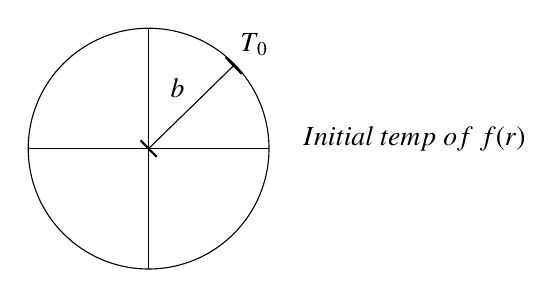
\begin{tikzpicture}[x=0.75pt,y=0.75pt,yscale=-1,xscale=1]
%uncomment if require: \path (0,300); %set diagram left start at 0, and has height of 300

%Shape: Circle [id:dp8517497421987501] 
\draw   (100,169) .. controls (100,136.97) and (125.97,111) .. (158,111) .. controls (190.03,111) and (216,136.97) .. (216,169) .. controls (216,201.03) and (190.03,227) .. (158,227) .. controls (125.97,227) and (100,201.03) .. (100,169) -- cycle ;
%Straight Lines [id:da20617477894091207] 
\draw    (100,169) -- (216,169) ;
%Straight Lines [id:da2792595315263553] 
\draw    (158,227) -- (158,111) ;
%Straight Lines [id:da4261506520298728] 
\draw    (158,169) -- (199,129) ;
\draw [shift={(199,129)}, rotate = 135.71] [color={rgb, 255:red, 0; green, 0; blue, 0 }  ][line width=0.75]    (0,5.59) -- (0,-5.59)   ;
\draw [shift={(158,169)}, rotate = 135.71] [color={rgb, 255:red, 0; green, 0; blue, 0 }  ][line width=0.75]    (0,5.59) -- (0,-5.59)   ;

% Text Node
\draw (176.5,145.6) node [anchor=south east] [inner sep=0.75pt]    {$b$};
% Text Node
\draw (201,125.6) node [anchor=south west] [inner sep=0.75pt]    {$T_{0}$};
% Text Node
\draw (231,157.4) node [anchor=north west][inner sep=0.75pt]    {$Initial\ temp\ of\ f( r)$};


\end{tikzpicture}

\end{center}

Because the source term \(Q/k\) is time‐independent, we can use a slave function:
\[
\psi(r,t) \;=\; \psi_{s}(r) \;+\; \Phi(r,t),
\]
where \(\psi_{s}(r)\) solves the steady-state (slave) ODE
\[
-\nabla^{2}\psi_{s} \;=\; \frac{Q}{k}, 
\qquad \psi_{s}(b)=T_{0},
\]
and \(\Phi(r,t)\) satisfies the homogeneous heat‐equation PDE with zero boundary conditions.

Using the polar‐coordinate Laplacian, \(-\nabla^{2}\psi_{s} = -\frac{1}{r}\frac{d}{dr}\!\bigl[r\,\psi_{s}'(r)\bigr]\), we get
\[
\frac{1}{r}\,\frac{d}{dr}\!\Bigl[r\,\frac{d\psi_{s}}{dr}\Bigr] \;=\; -\frac{Q}{k}.
\]
Multiply by \(r\) and integrate once:
\[
r\,\frac{d\psi_{s}}{dr} \;=\; -\frac{Q\,r^{2}}{2k} + C_{1}.
\]
Integrate again:
\[
\psi_{s}(r) 
= -\frac{Q\,r^{2}}{4k} + C_{1}\,\ln r + C_{2}.
\]
Finite behavior as \(r\to0\) forces \(C_{1}=0\).  Enforce \(\psi_{s}(b)=T_{0}\):
\[
\psi_{s}(b) = -\frac{Q\,b^{2}}{4k} + C_{2} = T_{0} 
\;\Longrightarrow\; 
C_{2} = T_{0} + \frac{Q\,b^{2}}{4k}.
\]
Hence
\[
\boxed{%
\psi_{s}(r) 
= \frac{Q}{4k}\bigl(b^{2} - r^{2}\bigr) + T_{0}.
}
\]

Next, \(\Phi(r,t)\) satisfies
\[
\frac{1}{\alpha^{2}}\frac{\partial \Phi}{\partial t} \;-\;\nabla^{2}\Phi \;=\;0,
\qquad
\begin{cases}
\Phi(b,t) = \psi(b,t) - \psi_{s}(b) = T_{0} - T_{0} = 0,\\
\Phi(r,0) = \psi(r,0) - \psi_{s}(r) = f(r) - \Bigl[\tfrac{Q}{4k}(b^{2} - r^{2}) + T_{0}\Bigr].
\end{cases}
\]
Denote 
\[
F(r) \;=\; f(r) \;-\; \frac{Q}{4k}\bigl(b^{2} - r^{2}\bigr) \;-\; T_{0}.
\]
Separation of variables \(\Phi(r,t) = R(r)\,T(t)\) yields
\[
\frac{1}{\alpha^{2}T}\,\frac{dT}{dt} 
\;=\; 
\frac{1}{r\,R}\,\frac{d}{dr}\!\Bigl[r\,\frac{dR}{dr}\Bigr] 
\;=\;\lambda.
\]
Thus the radial ODE is
\[
\frac{d}{dr}\!\Bigl[r\,\frac{dR}{dr}\Bigr]
= \lambda\,r\,R,
\]
and the temporal ODE is
\[
\frac{dT}{dt} = \alpha^{2}\,\lambda\,T.
\]

\textbf{Case 1: \(\lambda = 0\).}  Then \(T\) is constant and \(\frac{1}{r}\frac{d}{dr}[r\,R'] = 0\) implies \(R' \propto 1/r\), yielding a logarithmic or constant \(R\).  That cannot satisfy both \(R\) finite at \(r=0\) and \(R(b)=0\) nontrivially, so \(\lambda=0\) gives only the trivial \(\Phi\equiv0\) solution.

\textbf{Case 2: \(\lambda > 0\).} Write \(\lambda = \mu^{2}\).  Then
\[
\frac{dT}{dt} = \alpha^{2}\,\mu^{2}\,T \;\Longrightarrow\; T(t) = C\,e^{\alpha^{2}\mu^{2}t},
\]
which grows exponentially—unphysical for a diffusion problem with no additional sources in \(\Phi\).  Hence discard \(\lambda>0\).

\(\displaystyle\therefore\lambda < 0,\quad \lambda = -\,\mu^{2}.\)

Then the radial ODE becomes
\[
\frac{d}{dr}\!\Bigl[r\,\frac{dR}{dr}\Bigr] = -\,\mu^{2}\,r\,R,
\]
which in Sturm–Liouville form has \(p(r)=r,\;w(r)=r\).  Impose \(R\) finite at \(r=0\) and \(R(b)=0\).  Writing \(x = \mu\,r\), one gets Bessel’s equation of order zero:
\[
r^{2}\,R'' + r\,R' + \mu^{2}\,r^{2}\,R = 0 
\;\Longrightarrow\; 
x^{2}\,\frac{d^{2}R}{dx^{2}} + x\,\frac{dR}{dx} + x^{2}\,R = 0.
\]
The general solution is
\[
R(r) = A\,J_{0}(\mu\,r) + B\,Y_{0}(\mu\,r).
\]
Boundedness at \(r=0\) forces \(B=0\).  The condition \(R(b)=0\) implies
\[
J_{0}(\mu\,b) = 0,
\]
so let \(\{\beta_{k}\}\) be the positive zeros of \(J_{0}\).  Then \(\mu_{k} = \beta_{k}/b\) and
\[
\boxed{%
R_{k}(r) = J_{0}\!\bigl(\mu_{k}\,r\bigr),\quad
R_{k}(b) = 0,\quad k=1,2,3,\ldots.
}
\]
The temporal ODE is now
\[
\frac{dT}{dt} = -\,\alpha^{2}\,\mu^{2}\,T
\;\Longrightarrow\; 
T_{k}(t) = C_{k}\,e^{-\alpha^{2}\,\mu_{k}^{2}\,t}.
\]
Hence each separated mode is
\[
\Phi_{k}(r,t) = D_{k}\;J_{0}\bigl(\mu_{k}\,r\bigr)\;e^{-\alpha^{2} \mu_{k}^{2}\,t}.
\]
The general homogeneous solution is the superposition:
\[
\Phi(r,t)
= \sum_{k=1}^{\infty}
D_{k}\,J_{0}\bigl(\mu_{k}\,r\bigr)\,e^{-\alpha^{2}\,\mu_{k}^{2}\,t}.
\]
Enforce the initial condition \(\Phi(r,0) = F(r)\):
\[
F(r) 
= f(r) - \frac{Q}{4k}\bigl(b^{2}-r^{2}\bigr) - T_{0}
= \sum_{k=1}^{\infty} D_{k}\,J_{0}\bigl(\mu_{k}\,r\bigr).
\]
Since \(\{\,J_{0}(\mu_{k}r)\}\) is orthogonal on \([0,b]\) with weight \(r\):
\[
\int_{0}^{b} r\,J_{0}(\mu_{k}r)\,J_{0}(\mu_{\ell}r)\,dr = 0\quad(k\neq \ell),
\quad
\int_{0}^{b} r\,\bigl[J_{0}(\mu_{k}r)\bigr]^{2}\,dr 
= \frac{b^{2}}{2}\,\bigl[J_{1}(\beta_{k})\bigr]^{2}.
\]
Therefore
\[
D_{k}\,\int_{0}^{b} r\,\bigl[J_{0}(\mu_{k}r)\bigr]^{2}\,dr
= \int_{0}^{b} r\,F(r)\,J_{0}(\mu_{k}r)\,dr,
\]
\[
D_{k}\,\frac{b^{2}}{2}\,J_{1}(\beta_{k})^{2}
= \int_{0}^{b} r\,\Bigl[\,f(r) - \tfrac{Q}{4k}(b^{2}-r^{2}) - T_{0}\Bigr]\,
J_{0}(\mu_{k}r)\,dr.
\]
Hence
\[
\boxed{%
D_{k}
= \frac{2}{\,b^{2}\,J_{1}(\beta_{k})^{2}\,}\,
\int_{0}^{b} r\,\Bigl[f(r) - \tfrac{Q}{4k}(b^{2}-r^{2}) - T_{0}\Bigr]\,
J_{0}\!\bigl(\mu_{k}r\bigr)\,dr
\quad (k=1,2,\dots).
}
\]

Finally, the full solution is
\[
\boxed{%
\psi(r,t) 
= \psi_{s}(r) \;+\; \sum_{k=1}^{\infty}
\Bigl[\tfrac{2}{b^{2}J_{1}(\beta_{k})^{2}}\,
\int_{0}^{b} r\,\bigl(f(r) - \tfrac{Q}{4k}(b^{2}-r^{2}) - T_{0}\bigr)\,
J_{0}(\mu_{k}r)\,dr\Bigr]\,
J_{0}\!\bigl(\mu_{k}r\bigr)\,e^{-\alpha^{2}\,\mu_{k}^{2}\,t},
}
\]
where \(\psi_{s}(r) = \frac{Q}{4k}(b^{2} - r^{2}) + T_{0}\) and \(\mu_{k} = \beta_{k}/b\).

\section{BVP 11b : Vibrating Circular Membrane}

Clamped on the circumference \(r=b\), with initial displacement \(f(r)\) and initial velocity \(g(r)\).  A uniform gas pressure \(P\) acts downward on the membrane.  As in BVP 11a, there is no \(\theta\)-dependence, so \(\psi=\psi(r,t)\) satisfies
\[
a^{2}\,\nabla^{2}\psi \;-\; \frac{\partial^{2}\psi}{\partial t^{2}} \;=\; P,
\qquad
\begin{cases}
\text{B.C.:}& \psi(b,t) = 0,\\
\text{I.C.:}& \psi(r,0) = f(r),\quad \psi_{t}(r,0) = g(r),\quad \psi(0,t)\text{ finite.}
\end{cases}
\]

We write 
\[
\psi(r,t) \;=\; \psi_{s}(r) \;+\; \Phi(r,t),
\]
where \(\psi_{s}(r)\) solves the static (time-independent) problem:
\[
a^{2}\,\nabla^{2}\psi_{s} = P,
\qquad
\psi_{s}(b)=0,\quad \psi_{s}\text{ finite at }r=0.
\]
In polar coordinates, \(\nabla^{2}\psi_{s} = \frac{1}{r}(r\,\psi_{s}'(r))'\).  Hence
\[
\frac{1}{r}\,\frac{d}{dr}\!\Bigl[r\,\frac{d\psi_{s}}{dr}\Bigr] = \frac{P}{a^{2}}.
\]
Multiply by \(r\) and integrate:
\[
r\,\frac{d\psi_{s}}{dr} = \frac{P\,r^{2}}{2a^{2}} + C_{1},
\quad
\psi_{s}'(r) = \frac{P\,r}{2a^{2}} + \frac{C_{1}}{r}.
\]
Finiteness at \(r=0\) forces \(C_{1}=0\).  Integrate again and impose \(\psi_{s}(b)=0\):
\[
\psi_{s}(r) 
= \frac{P\,r^{2}}{4a^{2}} + C_{2}, 
\quad
\psi_{s}(b) = \frac{P\,b^{2}}{4a^{2}} + C_{2} = 0 
\;\Longrightarrow\; C_{2} = -\,\frac{P\,b^{2}}{4a^{2}}.
\]
Therefore
\[
\boxed{%
\psi_{s}(r) \;=\; \frac{P}{4a^{2}}\bigl(r^{2} - b^{2}\bigr).
}
\]

Next, \(\Phi(r,t)\) satisfies the homogeneous wave equation:
\[
a^{2}\,\nabla^{2}\Phi \;-\; \frac{\partial^{2}\Phi}{\partial t^{2}} = 0,
\qquad
\begin{cases}
\Phi(b,t) = \psi(b,t)\;-\;\psi_{s}(b) = 0 - 0 = 0,\\
\Phi(r,0) = \psi(r,0) - \psi_{s}(r) = f(r) - \frac{P}{4a^{2}}(r^{2}-b^{2}),\\
\Phi_{t}(r,0) = g(r).
\end{cases}
\]
Define 
\[
F(r) \;=\; f(r) \;-\; \frac{P}{4a^{2}}(r^{2}-\,b^{2}).
\]
Separation of variables \(\Phi(r,t) = R(r)\,T(t)\) leads to
\[
a^{2}\,\frac{1}{r\,R}\,\frac{d}{dr}\!\Bigl[r\,\frac{dR}{dr}\Bigr]
\;-\;
\frac{1}{T}\,\frac{d^{2}T}{dt^{2}}
\;=\;0
\;\Longrightarrow\;
\frac{1}{r\,R}\,\frac{d}{dr}\!\Bigl[r\,R'(r)\Bigr] 
= \frac{1}{a^{2}T}\,\frac{d^{2}T}{dt^{2}} 
= -\,\lambda.
\]
Thus the radial ODE is
\[
\frac{d}{dr}\!\Bigl[r\,\frac{dR}{dr}\Bigr] + \lambda\,r\,R = 0,
\quad 
R(b)=0,\;R\text{ finite at }r=0,
\]
and the temporal ODE is
\[
\frac{d^{2}T}{dt^{2}} + a^{2}\,\lambda\,T = 0.
\]

\textbf{Case 1: \(\lambda = 0\).}  Then \(\frac{d}{dr}[\,r\,R'(r)\,]=0\) implies \(R'(r)\propto 1/r\), yielding a logarithmic or constant solution, which cannot satisfy both \(R(b)=0\) and finiteness at \(r=0\) nontrivially.  Hence \(\lambda=0\) gives only the trivial \(\Phi\equiv0\).

\textbf{Case 2: \(\lambda < 0\).}  Write \(\lambda = -\,\mu^{2}\).  Then \(T'' - a^{2}\mu^{2}T = 0\) gives 
\[
T(t) = C\,\cos(a\mu\,t) + D\,\sin(a\mu\,t).
\]
The radial ODE becomes
\[
\frac{d}{dr}\!\Bigl[r\,\frac{dR}{dr}\Bigr] - \mu^{2}\,r\,R = 0,
\]
i.e.\ \(r^{2}R'' + r\,R' + \mu^{2}r^{2}R = 0\), Bessel’s equation of order zero.  Its general solution is
\[
R(r) = A\,J_{0}(\mu\,r) + B\,Y_{0}(\mu\,r).
\]
Boundedness at \(r=0\) forces \(B=0\).  Clamped boundary \(R(b)=0\) implies
\[
J_{0}(\mu\,b) = 0.
\]
Let \(\{\beta_{k}\}\) be the positive zeros of \(J_{0}\).  Then
\[
\mu_{k} = \frac{\beta_{k}}{b}, 
\quad
\boxed{%
R_{k}(r) = J_{0}\!\bigl(\mu_{k}\,r\bigr), 
\quad k=1,2,\dots
}
\]
The corresponding time‐modes are
\[
T_{k}(t) = C_{k}\,\cos(a\,\mu_{k}\,t) + D_{k}\,\sin(a\,\mu_{k}\,t).
\]
Hence 
\[
\Phi(r,t) 
= \sum_{k=1}^{\infty} J_{0}\!\bigl(\mu_{k}\,r\bigr)
\Bigl[c_{k}\,\cos\bigl(a\,\mu_{k}\,t\bigr)
+ D_{k}\,\sin\bigl(a\,\mu_{k}\,t\bigr)\Bigr].
\]
Apply the initial conditions:
\[
\Phi(r,0) = \sum_{k=1}^{\infty} c_{k}\,J_{0}\!\bigl(\mu_{k}\,r\bigr) 
= F(r),
\qquad
\Phi_{t}(r,0) = \sum_{k=1}^{\infty} D_{k}\,a\,\mu_{k}\,J_{0}\!\bigl(\mu_{k}\,r\bigr) 
= g(r).
\]
Orthogonality of \(\{\,J_{0}(\mu_{k}r)\}\) with weight \(r\) on \([0,b]\) gives
\[
\int_{0}^{b} r\,J_{0}(\mu_{k}r)\,J_{0}(\mu_{\ell}r)\,dr 
= 0\quad (k\neq \ell),
\quad
\int_{0}^{b} r\,[\,J_{0}(\mu_{k}r)\,]^{2}\,dr 
= \frac{b^{2}}{2}\,\bigl[J_{1}(\beta_{k})\bigr]^{2}.
\]
Hence
\[
C_{k}\,\frac{b^{2}}{2}\,J_{1}(\beta_{k})^{2} 
= \int_{0}^{b} r\,F(r)\,J_{0}(\mu_{k}r)\,dr,
\quad 
D_{k}\,a\,\mu_{k}\,\frac{b^{2}}{2}\,J_{1}(\beta_{k})^{2} 
= \int_{0}^{b} r\,g(r)\,J_{0}(\mu_{k}r)\,dr.
\]
Therefore
\[
\boxed{%
C_{k} = \frac{2}{\,b^{2}\,J_{1}(\beta_{k})^{2}\,}
\int_{0}^{b} r\,F(r)\,J_{0}\!\bigl(\mu_{k}r\bigr)\,dr,
\quad
D_{k} = \frac{2}{\,a\,\mu_{k}\,b^{2}\,J_{1}(\beta_{k})^{2}\,}
\int_{0}^{b} r\,g(r)\,J_{0}\!\bigl(\mu_{k}r\bigr)\,dr.
}
\]
Finally, the full solution is
\[
\boxed{%
\psi(r,t) 
= \frac{P}{4a^{2}}\bigl(r^{2} - b^{2}\bigr) 
\;+\; 
\sum_{k=1}^{\infty} J_{0}\!\bigl(\mu_{k}\,r\bigr)\,
\Bigl[C_{k}\,\cos\bigl(a\,\mu_{k} t\bigr) 
+ D_{k}\,\sin\bigl(a\,\mu_{k} t\bigr)\Bigr],
}
\]
where \(\mu_{k} = \beta_{k}/b\), and \(C_{k},D_{k}\) are as above.

\section{BVP 12: Diffusion of Heat in a Sphere}


There is no dependence on \(\theta\) or \(\varphi\), so \(\psi = \psi(r,t)\) satisfies
\[
\frac{1}{\alpha^{2}}\frac{\partial \psi}{\partial t}\;-\;\nabla^{2}\psi \;=\; \frac{Q}{k},
\qquad
\begin{cases}
\text{B.C.:}& \psi(b,t) = \beta,\\
\text{I.C.:}& \psi(r,0) = f(r),
\end{cases}
\]
where \(b\) is the sphere’s radius and \(\beta\) the surface temperature.

\begin{center}
    

\tikzset{every picture/.style={line width=0.75pt}} %set default line width to 0.75pt        

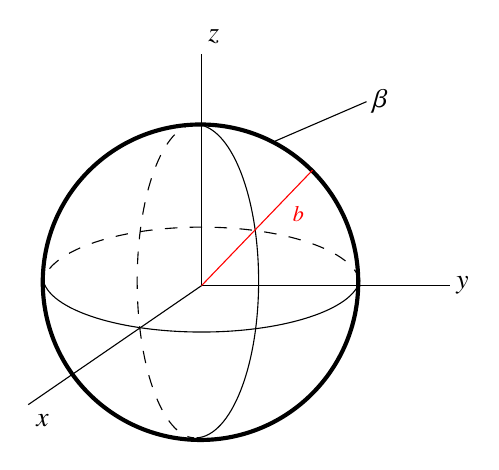
\begin{tikzpicture}[x=0.75pt,y=0.75pt,yscale=-1,xscale=1]
%uncomment if require: \path (0,511); %set diagram left start at 0, and has height of 511

%Shape: Circle [id:dp14934440830523532] 
\draw  [line width=1.5]  (84,156) .. controls (84,114.03) and (118.03,80) .. (160,80) .. controls (201.97,80) and (236,114.03) .. (236,156) .. controls (236,197.97) and (201.97,232) .. (160,232) .. controls (118.03,232) and (84,197.97) .. (84,156) -- cycle ;
%Shape: Arc [id:dp1214166957817917] 
\draw  [draw opacity=0] (236.72,155.33) .. controls (233.37,169.15) and (200.53,180) .. (160.5,180) .. controls (118.25,180) and (84,167.91) .. (84,153) -- (160.5,153) -- cycle ; \draw   (236.72,155.33) .. controls (233.37,169.15) and (200.53,180) .. (160.5,180) .. controls (118.25,180) and (84,167.91) .. (84,153) ;  
%Shape: Arc [id:dp4491292591346454] 
\draw  [draw opacity=0][dash pattern={on 4.5pt off 4.5pt}] (236.72,155.33) .. controls (233.51,140.84) and (200.6,129.45) .. (160.48,129.45) .. controls (118.23,129.45) and (83.98,142.08) .. (83.98,157.66) -- (160.48,157.66) -- cycle ; \draw  [dash pattern={on 4.5pt off 4.5pt}] (236.72,155.33) .. controls (233.51,140.84) and (200.6,129.45) .. (160.48,129.45) .. controls (118.23,129.45) and (83.98,142.08) .. (83.98,157.66) ;  
%Shape: Arc [id:dp2566153017664021] 
\draw  [draw opacity=0][dash pattern={on 4.5pt off 4.5pt}] (158.1,80.02) .. controls (157.9,80.01) and (157.69,80) .. (157.49,80) .. controls (142.03,80) and (129.49,113.8) .. (129.49,155.5) .. controls (129.49,196.71) and (141.74,230.21) .. (156.95,230.99) -- (157.49,155.5) -- cycle ; \draw  [dash pattern={on 4.5pt off 4.5pt}] (158.1,80.02) .. controls (157.9,80.01) and (157.69,80) .. (157.49,80) .. controls (142.03,80) and (129.49,113.8) .. (129.49,155.5) .. controls (129.49,196.71) and (141.74,230.21) .. (156.95,230.99) ;  
%Shape: Arc [id:dp8623515290830754] 
\draw  [draw opacity=0] (161.89,80.78) .. controls (176.66,86.06) and (188,117.5) .. (188,155.5) .. controls (188,196.75) and (174.63,230.28) .. (158.03,230.99) -- (157.49,155.5) -- cycle ; \draw   (161.89,80.78) .. controls (176.66,86.06) and (188,117.5) .. (188,155.5) .. controls (188,196.75) and (174.63,230.28) .. (158.03,230.99) ;  
%Straight Lines [id:da4169751367520922] 
\draw    (160.48,157.66) -- (280,157.66) ;
%Straight Lines [id:da615019222278173] 
\draw    (160.48,157.66) -- (160.48,46) ;
%Straight Lines [id:da31267781917423454] 
\draw    (160.48,157.66) -- (77,215) ;
%Straight Lines [id:da295919957911442] 
\draw [color={rgb, 255:red, 255; green, 0; blue, 0 }  ,draw opacity=1 ]   (160.48,157.66) -- (214,102) ;
%Straight Lines [id:da1215824133091894] 
\draw    (196,88) -- (240,69) ;

% Text Node
\draw (203.24,118.23) node [anchor=north west][inner sep=0.75pt]  [font=\footnotesize,color={rgb, 255:red, 255; green, 0; blue, 0 }  ,opacity=1 ]  {$b$};
% Text Node
\draw (79,218.4) node [anchor=north west][inner sep=0.75pt]    {$x$};
% Text Node
\draw (282,157.66) node [anchor=west] [inner sep=0.75pt]    {$y$};
% Text Node
\draw (162.48,42.6) node [anchor=south west] [inner sep=0.75pt]    {$z$};
% Text Node
\draw (242,69) node [anchor=west] [inner sep=0.75pt]    {$\beta $};


\end{tikzpicture}

\end{center}

Because \(Q/k\) is time‐independent, write
\[
\psi(r,t) \;=\; \psi_{s}(r) \;+\; \Phi(r,t),
\]
where \(\psi_{s}(r)\) solves the static ODE
\[
-\nabla^{2}\psi_{s} \;=\; \frac{Q}{k},
\qquad
\psi_{s}(b) = \beta,\quad \psi_{s}(0)\text{ finite}.
\]
In spherical coordinates (no angular terms),
\[
\nabla^{2}\psi_{s}
= \frac{1}{r^{2}}\frac{d}{dr}\!\Bigl[r^{2}\,\frac{d\psi_{s}}{dr}\Bigr].
\]
Thus
\[
-\frac{1}{r^{2}}\,\frac{d}{dr}\!\Bigl[r^{2}\,\frac{d\psi_{s}}{dr}\Bigr]
= \frac{Q}{k}
\;\Longrightarrow\;
\frac{d}{dr}\!\Bigl[r^{2}\,\frac{d\psi_{s}}{dr}\Bigr]
= -\,\frac{Q\,r^{2}}{k}.
\]
Integrate once:
\[
r^{2}\,\frac{d\psi_{s}}{dr}
= -\,\frac{Q\,r^{3}}{3k} + C_{1}
\;\Longrightarrow\;
\frac{d\psi_{s}}{dr}
= -\,\frac{Q\,r}{3k} + \frac{C_{1}}{r^{2}}.
\]
Finiteness at \(r=0\) forces \(C_{1}=0\).  Integrate again and impose \(\psi_{s}(b)=\beta\):
\[
\psi_{s}(r)
= -\,\frac{Q\,r^{2}}{6k} + C_{2},
\qquad
\psi_{s}(b) = -\,\frac{Q\,b^{2}}{6k} + C_{2} = \beta
\;\Longrightarrow\;
C_{2} = \beta + \frac{Q\,b^{2}}{6k}.
\]
Hence
\[
\boxed{%
\psi_{s}(r)
= \frac{Q}{6k}\,\bigl(b^{2} - r^{2}\bigr) + \beta.
}
\]

Next, \(\Phi(r,t)\) satisfies the homogeneous heat equation:
\[
\frac{1}{\alpha^{2}}\,\frac{\partial \Phi}{\partial t}
\;-\;
\nabla^{2}\Phi \;=\; 0,
\qquad
\begin{cases}
\Phi(b,t) = \psi(b,t) - \psi_{s}(b) = \beta - \beta = 0,\\
\Phi(r,0) = \psi(r,0) - \psi_{s}(r)
= f(r) - \Bigl[\frac{Q}{6k}(b^{2}-r^{2}) + \beta\Bigr].
\end{cases}
\]
Define 
\[
F(r) \;=\; f(r)\;-\;\frac{Q}{6k}\,(b^{2}-r^{2})\;-\;\beta.
\]
Separation of variables \(\Phi(r,t) = R(r)\,T(t)\) yields
\[
\frac{1}{\alpha^{2}T}\,\frac{dT}{dt}
\;=\;
\frac{1}{r^{2}R}\,\frac{d}{dr}\!\Bigl[r^{2}\,\frac{dR}{dr}\Bigr]
\;=\; -\,\lambda,
\]
so the radial ODE is
\[
\frac{d}{dr}\!\Bigl[r^{2}\,\frac{dR}{dr}\Bigr]
\;+\;\lambda\,r^{2}\,R \;=\; 0,
\qquad R(b)=0,\;R(0)\text{ finite},
\]
and the temporal ODE is
\[
\frac{dT}{dt} + \alpha^{2}\,\lambda\,T = 0 \;\Longrightarrow\; T(t) = e^{-\,\alpha^{2}\,\lambda\,t}.
\]

\textbf{Case 1: \(\lambda = 0\).}  Then \(\frac{d}{dr}[\,r^{2}R'\,]=0\implies R'\propto 1/r^{2}\), giving \(R(r)=C_{1}/r + C_{2}\).  Finiteness at \(r=0\) forces \(C_{1}=0\), and \(R(b)=0\) forces \(C_{2}=0\).  Hence \(R\equiv0\), trivial.

\textbf{Case 2: \(\lambda > 0\).}  Write \(\lambda = \mu^{2}\).  Then the radial ODE becomes
\[
\frac{d}{dr}\!\Bigl[r^{2}\,\frac{dR}{dr}\Bigr] + \mu^{2}\,r^{2}\,R = 0,
\]
i.e.\ 
\[
r^{2}\,R'' + 2r\,R' + \mu^{2}\,r^{2}\,R = 0,
\]
the spherical Bessel equation of order zero.  Its general solution is
\[
R(r) 
= \frac{A\sin(\mu\,r)}{r} + \frac{B\cos(\mu\,r)}{r}.
\]
Finiteness at \(r=0\) forces \(B=0\).  Clamped boundary \(R(b) = 0\) implies
\[
\frac{\sin(\mu\,b)}{b} = 0 
\;\Longrightarrow\;
\mu_{n}\,b = n\pi,\quad n=1,2,3,\dots
\;\Longrightarrow\;
\mu_{n} = \frac{n\pi}{b}.
\]
Thus 
\[
\boxed{%
R_{n}(r) = \frac{\sin\!\bigl(\tfrac{n\pi\,r}{b}\bigr)}{r}, 
\quad n = 1,2,\dots
}
\]
and
\[
T_{n}(t) = e^{-\,\alpha^{2}\,\mu_{n}^{2}\,t} = e^{-\,\alpha^{2}\,(n\pi/b)^{2}\,t}.
\]
Hence 
\[
\Phi(r,t) 
= \sum_{n=1}^{\infty} D_{n}\,\frac{\sin\!\bigl(\tfrac{n\pi\,r}{b}\bigr)}{r}\,
e^{-\,\alpha^{2}\,\bigl(\tfrac{n\pi}{b}\bigr)^{2}\,t}.
\]
Enforce the initial condition \(\Phi(r,0) = F(r)\):
\[
F(r) = \sum_{n=1}^{\infty} D_{n}\,\frac{\sin\!\bigl(\tfrac{n\pi\,r}{b}\bigr)}{r}.
\]
Multiply both sides by \(r\,\sin(\tfrac{m\pi\,r}{b})\) and integrate from \(0\) to \(b\).  Use
\[
\int_{0}^{b} \sin\!\Bigl(\tfrac{n\pi\,r}{b}\Bigr)\,\sin\!\Bigl(\tfrac{m\pi\,r}{b}\Bigr)\,dr
= 
\frac{b}{2}\,\delta_{nm}.
\]
Hence
\[
D_{n}\,\int_{0}^{b} \frac{\sin^{2}(\tfrac{n\pi\,r}{b})}{r}\,r\,dr
= 
\int_{0}^{b} r\,F(r)\,\sin\!\Bigl(\tfrac{n\pi\,r}{b}\Bigr)\,dr,
\]
\[
D_{n}\,\int_{0}^{b} \sin^{2}\!\Bigl(\tfrac{n\pi\,r}{b}\Bigr)\,dr
= 
\int_{0}^{b} r\,F(r)\,\sin\!\Bigl(\tfrac{n\pi\,r}{b}\Bigr)\,dr,
\]
and 
\(\displaystyle \int_{0}^{b} \sin^{2}\!\Bigl(\tfrac{n\pi\,r}{b}\Bigr)\,dr = \frac{b}{2}.\)
Therefore
\[
D_{n}\,\frac{b}{2} 
= 
\int_{0}^{b} r\,F(r)\,\sin\!\Bigl(\tfrac{n\pi\,r}{b}\Bigr)\,dr
\;\Longrightarrow\;
\boxed{%
D_{n}
= \frac{2}{\,b\,}\,
\int_{0}^{b} r\,F(r)\,\sin\!\Bigl(\tfrac{n\pi\,r}{b}\Bigr)\,dr,
\quad n=1,2,\dots
}
\]
with \(F(r) = f(r) - \tfrac{Q}{6k}(b^{2}-r^{2}) - \beta.\)

Finally, the full solution is
\[
\boxed{%
\psi(r,t) 
= \frac{Q}{6k}\bigl(b^{2} - r^{2}\bigr) + \beta
\;+\;\sum_{n=1}^{\infty} 
\Bigl[\tfrac{2}{b}\!\int_{0}^{b} r\,F(r)\,\sin(\tfrac{n\pi\,r}{b})\,dr\Bigr]\,
\frac{\sin(\tfrac{n\pi\,r}{b})}{r}\,
e^{-\,\alpha^{2}\,(n\pi/b)^{2}\,t}.
}
\]

\section{BVP 13: Steady-State Temp. in Annular Semicircle}

In polar coordinates \((r,\theta)\) on the domain 
\[
1 \;\le r \;\le e,\quad 0 \;\le \theta \;\le \pi,
\]
\(\psi(r,\theta)\) satisfies Laplace’s equation:
\[
\nabla^{2}\psi 
= \frac{1}{r}\,\frac{\partial}{\partial r}\!\Bigl[r\,\psi_{r}\Bigr]
+ \frac{1}{r^{2}}\,\frac{\partial^{2}\psi}{\partial \theta^{2}} 
= 0,
\]
with Dirichlet boundary conditions:
\[
\begin{aligned}
&\text{i) } \psi(1,\theta) = 0, 
\quad
\text{ii) } \psi(e,\theta) = 0,\\
&\text{iii) } \psi(r,0) = 0, 
\quad
\text{iv) } \psi(r,\pi) = f(r).
\end{aligned}
\]

\begin{center}
    

\tikzset{every picture/.style={line width=0.75pt}} %set default line width to 0.75pt        

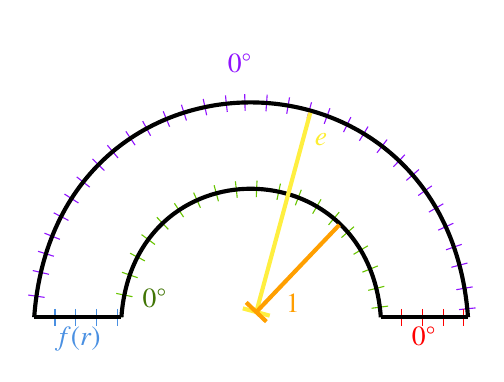
\begin{tikzpicture}[x=0.75pt,y=0.75pt,yscale=-1,xscale=1]
%uncomment if require: \path (0,511); %set diagram left start at 0, and has height of 511

%Straight Lines [id:da6083871249722499] 
\draw [color={rgb, 255:red, 74; green, 144; blue, 226 }  ,draw opacity=1 ]   (81,243.5) -- (123,243.5) (91,239.5) -- (91,247.5)(101,239.5) -- (101,247.5)(111,239.5) -- (111,247.5)(121,239.5) -- (121,247.5) ;
%Curve Lines [id:da7759696814398565] 
\draw [color={rgb, 255:red, 144; green, 19; blue, 254 }  ,draw opacity=1 ]   (81,243.5) .. controls (91,105) and (280,106) .. (290,243.5)(78.12,232.81) -- (86.04,233.94)(80.32,221.01) -- (88.11,222.82)(82.84,211.74) -- (90.47,214.13)(85.94,203) -- (93.37,205.97)(90.4,193.2) -- (97.51,196.85)(95.59,184.16) -- (102.33,188.48)(101.47,175.9) -- (107.76,180.84)(109.1,167.23) -- (114.8,172.84)(116.24,160.64) -- (121.38,166.77)(125.17,153.95) -- (129.61,160.6)(133.27,149.05) -- (137.09,156.08)(143.16,144.32) -- (146.23,151.71)(151.93,141.12) -- (154.35,148.74)(162.44,138.36) -- (164.09,146.19)(173.15,136.66) -- (174.02,144.61)(182.41,136.04) -- (182.62,144.03)(193.24,136.29) -- (192.67,144.27)(204.01,137.59) -- (202.66,145.48)(214.61,139.95) -- (212.49,147.66)(223.5,142.8) -- (220.73,150.31)(233.56,147.12) -- (230.03,154.3)(241.84,151.65) -- (237.68,158.49)(251.01,157.92) -- (246.16,164.27)(259.58,165.23) -- (254.06,171.02)(266.36,172.34) -- (260.31,177.58)(272.55,180.22) -- (266.03,184.86)(278.09,188.85) -- (271.16,192.85)(282.92,198.24) -- (275.65,201.56)(286.99,208.38) -- (279.43,211.01)(289.75,217.39) -- (282.01,219.44)(292.25,228.88) -- (284.37,230.24)(293.63,239.02) -- (285.67,239.82) ;
%Curve Lines [id:da7286710152328477] 
\draw [color={rgb, 255:red, 104; green, 196; blue, 0 }  ,draw opacity=1 ]   (123,243.5) .. controls (128.98,160.67) and (242.02,161.26) .. (248,243.5)(120.52,232.03) -- (128.36,233.61)(123.28,221.85) -- (130.84,224.47)(127.19,212.68) -- (134.31,216.34)(132.73,203.71) -- (139.18,208.45)(140.09,195.35) -- (145.6,201.15)(148.52,188.6) -- (152.97,195.25)(157.8,183.46) -- (161.09,190.75)(167.68,179.93) -- (169.77,187.65)(177.94,178) -- (178.81,185.95)(188.35,177.66) -- (188,185.66)(199.64,179.11) -- (197.96,186.93)(209.68,182.11) -- (206.8,189.57)(219.2,186.69) -- (215.15,193.59)(227.96,192.88) -- (222.81,199)(235.07,199.89) -- (229.03,205.13)(241.73,209.1) -- (234.87,213.2)(246.54,218.81) -- (239.11,221.79)(249.69,228.61) -- (241.93,230.55)(251.48,238.15) -- (243.55,239.18) ;
%Curve Lines [id:da5352280156604827] 
\draw [line width=1.5]    (81,243.5) .. controls (91,105) and (280,106) .. (290,243.5) ;
%Shape: Boxed Bezier Curve [id:dp8768995642015815] 
\draw [line width=1.5]    (123,243.5) .. controls (128.98,160.67) and (242.02,161.26) .. (248,243.5) ;
%Straight Lines [id:da4448377227820939] 
\draw [color={rgb, 255:red, 255; green, 0; blue, 0 }  ,draw opacity=1 ]   (248,243.5) -- (290,243.5) (258,239.5) -- (258,247.5)(268,239.5) -- (268,247.5)(278,239.5) -- (278,247.5)(288,239.5) -- (288,247.5) ;
%Straight Lines [id:da027318592126538643] 
\draw [line width=1.5]    (81,243.5) -- (123,243.5) ;
%Straight Lines [id:da4219949010453905] 
\draw [line width=1.5]    (248,243.5) -- (290,243.5) ;
%Straight Lines [id:da22515125565517247] 
\draw [color={rgb, 255:red, 255; green, 239; blue, 64 }  ,draw opacity=1 ][line width=1.5]    (188,241) -- (214,145) ;
\draw [shift={(188,241)}, rotate = 105.15] [color={rgb, 255:red, 255; green, 239; blue, 64 }  ,draw opacity=1 ][line width=1.5]    (0,6.71) -- (0,-6.71)   ;
%Straight Lines [id:da195137971937849] 
\draw [color={rgb, 255:red, 255; green, 159; blue, 0 }  ,draw opacity=1 ][line width=1.5]    (188,241) -- (228,199) ;
\draw [shift={(188,241)}, rotate = 133.6] [color={rgb, 255:red, 255; green, 159; blue, 0 }  ,draw opacity=1 ][line width=1.5]    (0,6.71) -- (0,-6.71)   ;

% Text Node
\draw (173,115.4) node [anchor=north west][inner sep=0.75pt]  [color={rgb, 255:red, 144; green, 19; blue, 254 }  ,opacity=1 ]  {$0^{\circ }$};
% Text Node
\draw (132,240.1) node [anchor=south west] [inner sep=0.75pt]  [color={rgb, 255:red, 65; green, 117; blue, 5 }  ,opacity=1 ]  {$0^{\circ }$};
% Text Node
\draw (201,237) node [anchor=west] [inner sep=0.75pt]  [color={rgb, 255:red, 255; green, 158; blue, 0 }  ,opacity=1 ]  {$1$};
% Text Node
\draw (215,153.4) node [anchor=north west][inner sep=0.75pt]  [color={rgb, 255:red, 253; green, 237; blue, 50 }  ,opacity=1 ]  {$e$};
% Text Node
\draw (102,246.9) node [anchor=north] [inner sep=0.75pt]  [color={rgb, 255:red, 74; green, 144; blue, 226 }  ,opacity=1 ]  {$f( r)$};
% Text Node
\draw (269,246.9) node [anchor=north] [inner sep=0.75pt]  [color={rgb, 255:red, 255; green, 0; blue, 0 }  ,opacity=1 ]  {$0^{\circ }$};


\end{tikzpicture}

\end{center}

Because the boundary at \(\theta=0\) is zero, we expand \(\psi\) in modes that vanish there.  Write
\[
\psi(r,\theta) 
= \sum_{n=1}^{\infty} R_{n}(r)\,\Theta_{n}(\theta).
\]
Each pair \((R_{n},\Theta_{n})\) satisfies the separated equations
\[
\frac{1}{r\,R_{n}}\frac{d}{dr}\!\Bigl[r\,\frac{dR_{n}}{dr}\Bigr]
\;+\;
\frac{1}{r^{2}\,\Theta_{n}}\frac{d^{2}\Theta_{n}}{d\theta^{2}} 
= 0,
\]
so
\[
\frac{1}{r^{2}\,\Theta_{n}}\,\frac{d^{2}\Theta_{n}}{d\theta^{2}}
= -\,\frac{1}{r\,R_{n}}\frac{d}{dr}\!\Bigl[r\,R_{n}'\Bigr]
= \lambda_{n} \quad (\text{separation constant}).
\]

\textbf{(a) Angular ODE.}  
\[
\Theta_{n}''(\theta) - \lambda_{n}\,\Theta_{n}(\theta) = 0,
\qquad
\Theta_{n}(0)=0,
\]
and there is no requirement that \(\Theta_{n}(\pi)=0\) (because \(\psi(r,\pi)=f(r)\) is nonzero).  To satisfy \(\Theta_{n}(0)=0\) and capture the nonhomogeneous BC at \(\theta=\pi\), choose \(\lambda_{n}=-\,\bigl(n\pi\bigr)^{2}<0\).  Then
\[
\Theta_{n}'' - \bigl(n\pi\bigr)^{2}\,\Theta_{n} = 0 
\;\Longrightarrow\; 
\Theta_{n}(\theta) = \sinh\!\bigl(n\pi\,\theta\bigr),
\quad 
\Theta_{n}(0)=0.
\]
At \(\theta=\pi\), \(\Theta_{n}(\pi) = \sinh\!\bigl(n\pi^{2}\bigr)\neq 0\).  

\textbf{(b) Radial ODE.}  
With \(\lambda_{n} = -\,n^{2}\pi^{2}\), the radial equation becomes
\[
r\,\frac{d}{dr}\!\Bigl[r\,R_{n}'(r)\Bigr] - \lambda_{n}\,r\,R_{n}(r) = 0
\;\Longleftrightarrow\;
r^{2}R_{n}'' + r\,R_{n}' + \bigl(n\pi\bigr)^{2}\,r^{2}\,R_{n} = 0.
\]
This is an Euler equation.  Seek \(R_{n}(r) = r^{k}\).  Then
\[
r^{2}\bigl[k(k-1)\,r^{k-2}\bigr] + r\bigl[k\,r^{k-1}\bigr] + (n\pi)^{2}\,r^{k} = 0
\;\Longrightarrow\;
\bigl[k^{2} + (n\pi)^{2}\bigr]\,r^{k} = 0
\;\Longrightarrow\;
k = \pm i\,n\pi.
\]
Hence the general radial solution is
\[
R_{n}(r) 
= A_{n}\,r^{\,i\,n\pi} \;+\; B_{n}\,r^{-\,i\,n\pi}
= A_{n}\,e^{\,i\,n\pi\,\ln r} \;+\; B_{n}\,e^{-\,i\,n\pi\,\ln r}.
\]
Real‐valued combinations give
\[
\boxed{%
R_{n}(r) = C_{n}\,\sin\!\bigl(n\pi\,\ln r\bigr),
}
\]
since \(\sin\bigl(n\pi\ln(1)\bigr)=0\) and \(\sin\bigl(n\pi\ln(e)\bigr) = \sin(n\pi)=0\).  Thus \(R_{n}(1)=R_{n}(e)=0\) are automatically satisfied for all integers \(n\ge1\).

\textbf{(c) Full separated modes.}  
\[
\psi_{n}(r,\theta) 
= R_{n}(r)\,\Theta_{n}(\theta)
= \sin\!\bigl(n\pi\,\ln r\bigr)\,\sinh\!\bigl(n\pi\,\theta\bigr).
\]
The general solution is
\[
\psi(r,\theta) 
= \sum_{n=1}^{\infty} E_{n}\,
\sin\!\bigl(n\pi\,\ln r\bigr)\,\sinh\!\bigl(n\pi\,\theta\bigr).
\]
Since \(\psi(r,0)=0\) is already satisfied, the only nonzero boundary is \(\psi(r,\pi)=f(r)\).  At \(\theta=\pi\):
\[
\psi(r,\pi) 
= \sum_{n=1}^{\infty} E_{n}\,\sin\!\bigl(n\pi\,\ln r\bigr)\,\sinh\!\bigl(n\pi^{2}\bigr)
\;\stackrel{!}{=}\; f(r).
\]
Define 
\[
F(r) \;=\; f(r).
\]
Expand \(F(r)\) in the orthogonal basis \(\{\sin(n\pi\ln r)\}\) with weight \(w(r)=1/r\) on \(r\in[1,e]\).  Note the inner product:
\[
\int_{1}^{e} \frac{1}{r}\,\sin\!\bigl(n\pi\,\ln r\bigr)\,
\sin\!\bigl(m\pi\,\ln r\bigr)\,dr 
= \int_{0}^{1} \sin(n\pi x)\,\sin(m\pi x)\,dx
= \frac{1}{2}\,\delta_{nm}.
\]
Hence
\[
E_{n}\,\sinh\!\bigl(n\pi^{2}\bigr)\,\int_{1}^{e} \frac{1}{r}\,\sin^{2}\!\bigl(n\pi\,\ln r\bigr)\,dr
= \int_{1}^{e} \frac{F(r)}{r}\,\sin\!\bigl(n\pi\,\ln r\bigr)\,dr,
\]
and since \(\int_{1}^{e}\frac{1}{r}\sin^{2}(n\pi\ln r)\,dr = \tfrac12\), we get
\[
\boxed{%
E_{n}
= \frac{2}{\,\sinh\!\bigl(n\pi^{2}\bigr)\,}\,
\int_{1}^{e} \frac{f(r)}{r}\,\sin\!\bigl(n\pi\,\ln r\bigr)\,dr,
\quad
\psi(r,\theta) 
= \sum_{n=1}^{\infty}\!
\Bigl[\tfrac{2}{\sinh(n\pi^{2})}\!\int_{1}^{e}\tfrac{f(r)}{r}\,\sin(n\pi\ln r)\,dr\Bigr]\,
\sin\bigl(n\pi\ln r\bigr)\,\sinh\bigl(n\pi\,\theta\bigr).
}
\]
This series satisfies 
\(\psi(1,\theta)=0\), \(\psi(e,\theta)=0\), 
\(\psi(r,0)=0\), and \(\psi(r,\pi)=f(r)\).

\end{document}
